% filepath: D:\TAI LIEU HOC TAP\Thesis\main.tex
% !TeX root = main.tex
% Template KLTN cho SV trường ĐHKHTN
% Liên hệ: nqminh@fit.hcmus.edu.vn
% Last update: 08/06/2016

% Chú ý: đọc các phần chú ý đóng khung của file này và chỉnh lại cho phù hợp.
% Trước khi build, xóa hết các file được tạo ra trong quá trình build trước đó, và build theo thứ tự: BIB > PDF > PDF.
% Nếu cập nhật tài liệu tham khảo, cũng cần build lại theo cách trên.

\documentclass[oneside,a4paper,14pt]{extreport}
\usepackage[fontsize=13pt]{scrextend}
% Font tiếng Việt
\usepackage[T5]{fontenc}
\usepackage[utf8]{inputenc}
\usepackage{mathptmx}
\usepackage{fancyhdr}
\usepackage{subcaption}
\usepackage{titlesec}
\usepackage{diagbox}
\usepackage{amssymb}
\setcounter{secnumdepth}{4}
\DeclareTextSymbolDefault{\DH}{T1}

% Tài liệu tham khảo
\usepackage[
	sorting=nty,
	backend=bibtex,
	defernumbers=true]{biblatex}
\usepackage[unicode]{hyperref} % Bookmark tiếng Việt
\addbibresource{References/references.bib}

\makeatletter
\def\blx@maxline{77}
\makeatother

% Chèn hình, các hình trong luận văn được để trong thư mục Images/
\usepackage{graphicx}
\graphicspath{ {Images/} }

% Chèn và định dạng mã nguồn
\usepackage{listings}
\usepackage{color}
\definecolor{codegreen}{rgb}{0,0.6,0}
\definecolor{codegray}{rgb}{0.5,0.5,0.5}
\definecolor{codepurple}{rgb}{0.58,0,0.82}
\definecolor{backcolour}{rgb}{0.95,0.95,0.92}
\lstdefinestyle{mystyle}{
    backgroundcolor=\color{backcolour},   
    commentstyle=\color{codegreen},
    keywordstyle=\color{magenta},
    numberstyle=\tiny\color{codegray},
    stringstyle=\color{codepurple},
    basicstyle=\footnotesize,
    breakatwhitespace=false,         
    breaklines=true,                 
    captionpos=b,                    
    keepspaces=true,                 
    numbers=left,                    
    numbersep=5pt,                  
    showspaces=false,                
    showstringspaces=false,
    showtabs=false,                  
    tabsize=2
}
\lstset{style=mystyle}

% Chèn và định dạng mã giả
\usepackage{amsmath}
\usepackage{algorithm}
\usepackage[noend]{algpseudocode}
\makeatletter
\def\BState{\State\hskip-\ALG@thistlm}
\makeatother

% Bảng biểu
\usepackage{multirow}
\usepackage{array}
\newcolumntype{L}[1]{>{\raggedright\let\newline\\\arraybackslash\hspace{0pt}}m{#1}}
\newcolumntype{C}[1]{>{\centering\let\newline\\\arraybackslash\hspace{0pt}}m{#1}}
\newcolumntype{R}[1]{>{\raggedleft\let\newline\\\arraybackslash\hspace{0pt}}m{#1}}



 
% Đổi tên mặc định
\renewcommand{\chaptername}{Chương}
\renewcommand{\figurename}{Hình}
\renewcommand{\tablename}{Bảng}
\renewcommand{\contentsname}{Mục lục}
\renewcommand{\listfigurename}{Danh sách hình}
\renewcommand{\listtablename}{Danh sách bảng}
\renewcommand{\appendixname}{Phụ lục}

\usepackage{titlesec}

\setcounter{secnumdepth}{3}

\titleformat{\chapter}
    [block]
    {\filcenter\normalfont\bfseries\normalsize}{\chaptername \ \thechapter :}{10pt}{\normalsize}
\titlespacing*{\chapter}{0pt}{-10pt}{10pt} %khoảng cách giữa chapter và đầu trang

\titleformat{\section}
    {\normalfont\bfseries\normalsize}{\thesection}{1em}{}
 
\titleformat{\subsection}
    {\normalfont\bfseries\normalsize}{\thesubsection}{1em}{}

\titleformat{\subsubsection}
    {\normalfont\bfseries\normalsize}{\thesubsubsection}{1em}{}
  
% Dãn dòng 1.5
\usepackage{setspace}
\onehalfspacing

% Thụt vào đầu dòng
\usepackage{indentfirst}

% Canh lề
\usepackage[
  top=20mm,
  bottom=10mm,
  left=30mm,
  right=20mm,
  footskip = 15mm,
  includefoot]{geometry}
  
% Dãn dòng 1.5
\usepackage{setspace}
\onehalfspacing

% Thụt vào đầu dòng
\usepackage{indentfirst}

% Canh lề
\usepackage[
  top=20mm,
  bottom=10mm,
  left=30mm,
  right=20mm,
  footskip = 15mm,
  includefoot]{geometry}
  
% Trang bìa
\usepackage{tikz}
\usetikzlibrary{calc}
\newcommand\HRule{\rule{\textwidth}{1pt}}

% ========================================================================================= %
% CHÚ Ý: Thông tin chung về KLTN - sinh viên điền vào đây để tự động update các trang khác  %
% ========================================================================================= %
\newcommand{\tenSV}{Nguyễn~Văn~A~-~Trần~Văn~B} % Dấu ~ là khoảng trắng không được tách (các chữ nối với nhau bằng dấu ~ sẽ nằm cùng 1 dòng
\newcommand{\mssv}{1234567}
\newcommand{\tenKL}{Sử~dụng~LaTeX trong Khoá~luận~tốt~nghiệp} % Chú ý dấu ~ trong tên khóa luận
\newcommand{\tenGVHD}{Tên~Giáo~Viên}
\newcommand{\tenBM}{Công nghệ tri thức}

\begin{document}
\pagestyle{fancy}
\fancyhf{}
\fancyfoot[R]{\thepage}
\renewcommand{\headrulewidth}{0pt}
\renewcommand{\footrulewidth}{0pt}

\fancypagestyle{plain}{
  \fancyhf{}
  \fancyfoot[R]{\thepage}
  \renewcommand{\headrulewidth}{0pt}
  \renewcommand{\footrulewidth}{0pt}
}

\let\oldchapter\chapter
\renewcommand{\chapter}{%
  \cleardoublepage%
  \pagestyle{fancy}%
  \oldchapter}


\begin{titlepage}
\thispagestyle{empty}
\begin{center}
%ĐẠI HỌC QUỐC GIA THÀNH PHỐ HỒ CHÍ MINH\\
TRƯỜNG ĐẠI HỌC KHOA HỌC TỰ NHIÊN\\
\textbf{KHOA ĐIỆN TỬ - VIỄN THÔNG}\\
\textbf{BỘ MÔN MÁY TÍNH - HỆ THỐNG NHÚNG}\\[2cm]



{ \Large \bfseries Hoàng Hữu Tú\\[2cm] } 

%Tên đề tài Khóa luận tốt nghiệp/Đồ án tốt nghiệp

{ \Large \bfseries PHÁT TRIỂN KIẾN TRÚC BẢO MẬT HỆ THỐNG IOT SỬ DỤNG KHUNG TRUYỀN DỮ LIỆU KẾT HỢP CƠ CHẾ TRAO ĐỔI KHÓA ĐỘNG VÀ KỸ THUẬT MẬT MÃ HÓA NHẸ ASCON\\[3cm]} 


%Chọn trong các dòng sau
% \large KHÓA LUẬN TỐT NGHIỆP CỬ NHÂN\\
\Large \bfseries Chuyên ngành Máy Tính - Hệ Thống Nhúng
%\large ĐỒ ÁN TỐT NGHIỆP CỬ NHÂN\\
%\large THỰC TẬP TỐT NGHIỆP CỬ NHÂN\\
%Đưa vào dòng này nếu thuộc chương trình Chất lượng cao, hoặc lớp Cử nhân tài năng
% \large CHƯƠNG TRÌNH CHÍNH QUY\\
%\large CHƯƠNG TRÌNH CHẤT LƯỢNG CAO\\
%\large CHƯƠNG TRÌNH CỬ NHÂN TÀI NĂNG\\[2cm]


\begin{tikzpicture}[remember picture, overlay]
  \draw[line width = 2pt] ($(current page.north west) + (2cm,-2cm)$) rectangle ($(current page.south east) + (-1.5cm,2cm)$);
\end{tikzpicture}

\vfill
Tp. Hồ Chí Minh, tháng 07/2025

\end{center}

\pagebreak


\thispagestyle{empty}
\begin{center}

TRƯỜNG ĐẠI HỌC KHOA HỌC TỰ NHIÊN\\
\textbf{KHOA ĐIỆN TỬ - VIỄN THÔNG}\\
\textbf{BỘ MÔN MÁY TÍNH - HỆ THỐNG NHÚNG}\\[2cm]


{\large \bfseries Hoàng Hữu Tú\\} 
{\large \bfseries 21200249\\[1.5cm]} 
% {\large \bfseries Trần Thị B - 1512007\\}

%Tên đề tài Khóa luận tốt nghiệp/Đồ án tốt nghiệp

{ \large \bfseries PHÁT TRIỂN KIẾN TRÚC BẢO MẬT HỆ THỐNG IOT SỬ DỤNG KHUNG TRUYỀN DỮ LIỆU KẾT HỢP CƠ CHẾ TRAO ĐỔI KHÓA ĐỘNG VÀ KỸ THUẬT MẬT MÃ HÓA NHẸ ASCON\\[1cm] } 
{ \large \bfseries IMPLEMENTATION OF A SECURE IOT ARCHITECTURE USING A CUSTOM TRANSMISSION FRAME WITH DYNAMIC KEY EXCHANGE AND ASCON LIGHTWEIGHT CRYPTOGRAPHY\\[2cm] } 

%Chọn trong các dòng sau
\large KHÓA LUẬN TỐT NGHIỆP CỬ NHÂN\\
%\large ĐỒ ÁN TỐT NGHIỆP CỬ NHÂN\\
%Đưa vào dòng này nếu thuộc chương trình Chất lượng cao, hoặc lớp Cử nhân tài năng
\large NGÀNH KỸ THUẬT ĐIỆN TỬ VIỄN THÔNG\\
\large CHUYÊN NGÀNH MÁY TÍNH - HỆ THỐNG NHÚNG\\[1.5cm]
%\large CHƯƠNG TRÌNH CHẤT LƯỢNG CAO\\[2cm]
%\large CHƯƠNG TRÌNH CỬ NHÂN TÀI NĂNG\\[2cm]

\textbf{NGƯỜI HƯỚNG DẪN KHOA HỌC}\\
PGS.TS. Lê Đức Hùng \\
ThS. Cao Trần Bảo Thương

\begin{tikzpicture}[remember picture, overlay]
  \draw[line width = 2pt] ($(current page.north west) + (2cm,-2cm)$) rectangle ($(current page.south east) + (-1.5cm,2cm)$);
\end{tikzpicture}

\vfill
Tp. Hồ Chí Minh, tháng 07/2025

\end{center}

\end{titlepage}
% Sasu trang Title, các bạn chèn nhận xét gủa GVHD và GVPB. Nhận xét sẽ được giáo vụ phát sau buổi bảo vệ để các bạn đóng quyển.

\pagenumbering{roman} % Đánh số i, ii, iii, ...

\addcontentsline{toc}{chapter}{Lời cam đoan}
\chapter*{Lời cam đoan}
\label{reassurances}

Tôi xin cam đoan những số liệu và kết quả nghiên cứu được trình bày trong khóa luận tốt nghiệp
là trung thực. Tôi cam kết không sao chép nội dung hay kết quả của các nghiên cứu khác đã được công bố. Những tài liệu tham khảo được tôi sử dụng trong báo cáo đã được trích dẫn một cách đầy đủ, rõ ràng về nguồn gốc theo quy định.

Tôi xin chịu trách nhiệm nếu vi phạm các cam kết trên.

\begin{table}[h]
\begin{tabular}{p{0.6\textwidth}p{0.4\textwidth}}
 &
 \begin{center}

\vspace{2cm}
\tenSV
 \end{center}
\end{tabular}
\end{table}

\addcontentsline{toc}{chapter}{Lời cảm ơn}
\chapter*{Lời cảm ơn}
\label{thanks}

Lời đầu tiên, em xin gửi lời cảm ơn sâu sắc tới thầy PGS.TS. Lê Đức Hùng. 
Trong thời gian qua, thầy đã giúp đỡ và chỉ bảo rất tận tình cho em để 
có thể hoàn thành khóa luận tốt nghiệp này. Hơn thế nữa, thầy đã tạo
cơ hội và điều kiện để em có thể có được bài báo khoa học đầu tiên được chấp nhận,
đóng góp vào sự nghiệp nghiên cứu khoa học, và là một thành tựu lớn của bản thân em trong quãng đời 
sinh viên.

Tiếp theo, em xin gửi lời cảm ơn đến anh Nguyễn Vũ Minh Thành đã giúp đỡ em
rất nhiều trong thời gian qua. Trong giai đoạn sơ khai và hình thành dự án, anh Thành
đã giúp em góp ý cũng như đề xuất các ý tưởng hay để có thể triển khai một hệ thống
hoàn thiện như bây giờ. 

Đặc biệt, em xin chân thành cảm ơn các thành viên trong phòng thí 
nghiệm DESLab. DESLab đã cho em môi trường lý tưởng để làm việc và
phát triển. Trong suốt thời gian ở phòng thí nghiệm, em đã học tập được
rất nhiều không chỉ là về kỹ năng chuyên môn mà còn cả về tinh thần làm
việc nghiêm túc và tư duy trong nghiên cứu khoa học. Gia nhập vào DESLab
chính là bước ngoặt lớn nhất trong suốt bốn năm đại học, em sẽ luôn nhớ về DESLab
là nơi đầu tiên đã giúp em định hình và phát triển được như bây giờ. 

Em xin gửi lời cảm ơn chân thành đến gia đình – những người luôn âm thầm ủng hộ, động viên và là chỗ dựa tinh thần vững chắc để em vững bước trong suốt hành trình học tập và trưởng thành.

Sau cùng, em xin cảm ơn tới quý thầy, cô khoa Điện Tử - Viễn Thông. 
Các thầy, cô đã giúp đỡ em rất nhiều trong quá trình học tập và nghiên cứu.

\begin{table}[h]
\begin{tabular}{p{0.6\textwidth}p{0.4\textwidth}}
 &
 \begin{center}
\tenSV
 \end{center}
\end{tabular}
\end{table}

\addcontentsline{toc}{chapter}{Đề cương chi tiết}
\include{Appendix/decuong}

% Mục lục, danh sách hình, danh sách bảng
\addcontentsline{toc}{chapter}{Mục lục}
\tableofcontents
\listoffigures
\listoftables

\addcontentsline{toc}{chapter}{Tóm tắt}
\include{Appendix/tomtat}

\clearpage

\pagenumbering{arabic} % Đánh số 1, 2, 3, ...

% Các chương nội dung
\chapter{Giới thiệu}
\label{Chapter1}

Chương \ref{Chapter1}    đưa ra các nội dung tổng quan của khóa luận tốt nghiệp. Trong đó, các
nội dung được trình bày là việc đặt vấn đề, mục tiêu hướng tới, giải pháp đề xuất,
đóng góp, và bố cục của khóa luận.

\section{Đặt vấn đề}
\label{sec:prob}
Internet of Things (IoT) đã và đang trở thành một trong những trụ cột quan trọng trong sự phát triển của các công nghệ hiện đại, mở ra nhiều đột phá trong các lĩnh vực như chăm sóc sức khỏe, tự động hóa và các hệ thống thông minh \cite{iot1}. Tuy nhiên, phần lớn các thiết bị IoT hiện nay đều hoạt động trong môi trường có tài nguyên hạn chế, bao gồm tốc độ xử lý thấp, dung lượng pin hạn chế, cũng như kết nối mạng không ổn định. Những hạn chế này khiến các thiết bị dễ bị ảnh hưởng trước các mối đe dọa về bảo mật \cite{iot2}, làm gia tăng nguy cơ mất gói tin trong quá trình truyền dữ liệu. Những kẻ tấn công thường lợi dụng các điểm yếu này để khai thác các lỗ hổng bảo mật trong phần cứng, phần mềm và giao thức để nhắm vào hệ sinh thái IoT trong các hệ thống doanh nghiệp, công nghiệp và chính phủ. Do đó, tính bảo mật, tính toàn vẹn và tính khả dụng của các hệ thống này bị suy yếu gây ra các thiệt hại vô cùng lớn.
% như nghe lén trái phép (eavesdropping), chỉnh sửa dữ liệu (tampering) và tấn công phát lại (replay attack), trong đó các gói tin hợp lệ bị kẻ tấn công phát lại với mục đích xấu \cite{?}. 

Để xây dụng một hệ thống IoT bảo mật yêu cầu phải có một thuật toán mã hóa đủ mạnh. Các thuật toán mã hóa truyền thống như AES hoặc RSA, tuy hiệu quả và phổ biến trong các hệ thống có tài nguyên dồi dào, lại gặp nhiều khó khăn khi triển khai trên các thiết bị IoT do yêu cầu cao về tính toán và bộ nhớ \cite{iot3}. Vì vậy, khi triển khai hệ thống IoT phải cân nhắc các thuật toán mã hóa nhẹ, phù hợp với các thiết bị IoT hiện nay. Một điều cần chú trọng đó là khi thiết kế các hệ thống IoT, cần xem xét các cơ chế bảo mật ở nhiều lớp \cite{iot4}. Đối với mô hình hệ thống IoT bốn lớp, các lớp trung gian như lớp nhận thức (perceptual layer), lớp mạng (network layer) và lớp xử lý dữ liệu (data processing layer) cần được xem xét để tăng cường bảo mật cũng như đảm bảo tính toàn vẹn của dữ liệu. Tại lớp nhận thức, các giao thức truyền thông đơn giản như UART (Universal Asynchronous Receiver-Transmitter) thường được sử dụng do tính nhẹ và phù hợp với phần lớn các thiết bị tài nguyên thấp. Tuy nhiên, việc truyền dữ liệu thô lại tiềm ẩn nguy cơ mất mát gói tin và tiếp nhận dữ liệu không được xác thực từ các nguồn không tin cậy \cite{iot5}. Bên cạnh đó, trong quá trình truyền dữ liệu giữa gateway và máy chủ, việc mã hóa dữ liệu là bắt buộc; đồng thời, các khóa bí mật sử dụng trong quá trình mã hóa và giải mã cần được thay đổi định kỳ nhằm giảm thiểu nguy cơ bị tấn công dò khóa. Thực tế, nhiều thiết bị IoT cấp thấp hiện nay gặp vấn đề trong việc quản lý khóa bí mật, thường sử dụng các khóa tĩnh được cài đặt sẵn hoặc dựa vào bộ đếm để tạo khóa, dẫn đến nguy cơ bị phá vỡ bảo mật do các phương pháp tấn công tinh vi \cite{iot6}.

Do đó, việc nghiên cứu và phát triển các giải pháp bảo mật nhẹ, phù hợp với tài nguyên hạn chế của thiết bị IoT, đồng thời đảm bảo các yếu tố như dữ liệu phải được mã hóa, khả năng kháng lại các cuộc tấn công, đảm bảo tính toàn vẹn của dữ liệu, các lớp trong kiến trúc IoT đều phải có cơ chế bảo mật hợp lý là một yêu cầu cấp thiết để nâng cao độ an toàn và hiệu quả của các hệ thống IoT trong thực tiễn.

\section{Mục tiêu của đề tài}
Các thiết bị IoT tài nguyên thấp thường dễ bị khai thác do thiếu các cơ chế bảo mật mạnh mẽ, chẳng hạn như mã hóa phức tạp hoặc xác thực thời gian thực cũng như một số nhược điểm khác
được đề cập ở phần \ref{sec:prob}. 
Hơn nữa, phần lớn các nghiên cứu trong lĩnh vực bảo mật IoT chỉ tập trung giải quyết các bài toán đơn lẻ hoặc dừng lại ở mức lý thuyết. Vì vậy, đề tài hướng đến việc thiết kế một kiến trúc IoT hoàn chỉnh, có khả năng triển khai trên các thiết bị phần cứng khác nhau, đặc biệt là những thiết bị có tài nguyên giới hạn. Kiến trúc phải 
đảm bảo khả năng bảo mật đa lớp trong kiến trúc IoT bốn lớp. Từ đó, đề tài hướng đến việc đóng góp cho cộng đồng một kiến trúc có tính tổng quát cao, có thể triển khai trên bất kỳ nền tảng phần cứng nào.

\section{Giải pháp đề xuất}
Đề tài tập trung vào phát triển một kiến trúc IoT bảo mật toàn diện, vừa đảm bảo các yếu tố an toàn như tính toàn vẹn, bí mật dữ liệu, và khả năng chống lại các cuộc tấn công từ bên ngoài, vừa tối ưu để phù hợp với các thiết bị có tài nguyên hạn chế. Kiến trúc đề xuất sẽ tích hợp các giải pháp như sử dụng thuật toán mã hóa nhẹ, cơ chế trao đổi khóa động và kiến trúc khung truyền riêng đảm bảo chỉ có các thiết bị được ủy quyền mới có thể xử lý và giải mã các gói tin hợp lý. Đề tài cũng giới thiệu phương pháp \textit{safe counter} mới nhằm hạn chế khả năng bị brute-force vào các gói tin. Qua đó, hệ thống vừa tăng cường bảo mật truyền thông giữa các lớp vừa duy trì hiệu suất và tính khả thi, đáp ứng nhu cầu thực tiễn trong các lĩnh vực y tế, giao thông và nhà thông minh.

\section{Đóng góp của đề tài}
Kết quả của khóa luận là những đóng góp trong việc thiết kế một kiến trúc IoT bảo mật, tối ưu cho các thiết bị tài nguyên thấp. Trong truyền dữ liệu, thuật toán mã hóa Ascon-128a đã được áp dụng nhằm đảm bảo tính bảo mật trong hệ thống, giảm đáng kể độ trễ mã hóa so với AES. Các gói tin được định dạng trong cấu trúc khung truyền tùy chỉnh, tích hợp các trường như header đồng bộ, định danh, số thứ tự, và mã xác thực,... giúp xác minh tính toàn vẹn và ngăn chặn một số cuộc tấn công. Trao đổi khóa Elliptic Curve Diffie-Hellman (ECDH) sử dụng đường cong \textit{sect163k1} kết hợp với kỹ thuật tạo khóa phiên dùng hàm băm Ascon Hash được triển khai hiệu quả, cho phép tạo khóa bí mật động giữa gateway (ESP32) và máy chủ, tăng cường bảo mật trước các tấn công Man-in-the-Middle. Các kết quả thử nghiệm sử dụng vi điều khiển tầm trung như STM32F411VET6 và ESP32 cho thấy tỷ lệ truyền gói tin đạt 99.99\% trong 120 phút (147,682 gói tin), độ trễ trung bình 51.08 ms, và khả năng từ chối 100\% 70,000 gói tin phát lại, khẳng định tính ổn định và an toàn của khung đề xuất. 

\section{Bố cục của khóa luận}

Báo cáo khóa luận được chia thành 5 chương gồm các nội dung như sau:
\begin{itemize}
    \item CHƯƠNG 1: GIỚI THIỆU
    \item CHƯƠNG 2: CÁC CÔNG TRÌNH LIÊN QUAN
    \item CHƯƠNG 3: PHƯƠNG PHÁP ĐỀ XUẤT
    \item CHƯƠNG 4: KẾT QUẢ TRIỂN KHAI VÀ PHÂN TÍCH
    \item CHƯƠNG 5: KẾT LUẬN
\end{itemize}

Chương 1 sẽ đưa ra các nội dung tổng quát của khóa luận. Các nội dung chính 
bao gồm đặt vấn đề, mục tiêu của đề tài, đóng góp của đề tài, và bố cục của khóa luận.

Chương 2 sẽ đưa ra một số công trình liên quan đến đề tài, làm rõ các ưu nhược điểm của từng công trình.
Ngoài ra, chương này cũng sẽ phân tích một số cuộc tấn công phổ biến trong hệ thống IoT. Từ đó, đưa ra khoảng trống nghiên cứu, 
các vấn đề mà đề tài tập trung giải quyết.

Chương 3 bao gồm hai phần chính. Phần thứ nhất tập trung về cơ sở lý thuyết liên quan tới kiến trúc IoT đề xuất. Phần thứ hai sẽ trình bày
chi tiết quá trình triển khai từng module trong hệ thống.

Chương 4 đưa ra các kết quả đạt được trong việc triển khai. Đồng thời, chương này sẽ đánh giá hiệu suất và một số thông số quan trọng khác cũng như
phân tích và nhận xét về khả năng bảo mật của hệ thống.

Cuối cùng là chương 5 sẽ tóm gọn lại về mục tiêu, phương pháp, kết quả đạt được. Đồng thời sẽ đưa ra các hạn chế của đề tài và 
đề xuất hướng phát triển trong tương lai.
% Tóm lại, các vấn đề bảo mật chính mà các hệ thống IoT hiện nay đang đối mặt bao gồm:
% \begin{enumerate}
%     \item Hạn chế tài nguyên: Các thiết bị IoT thường bị giới hạn về khả năng tính toán và tài nguyên, gây khó khăn trong việc triển khai các thuật toán mã hóa phức tạp.
%     \item Mất mác và không xác thực dữ liệu: Việc sử dụng các giao thức truyền thông đơn giản dễ dẫn đến mất gói tin hoặc tiếp nhận dữ liệu từ nguồn không đáng tin cậy. 
%     \item Quản lý khóa bí mật: Việc sử dụng khóa tĩnh hoặc các phương pháp tạo khóa không an toàn làm tăng nguy cơ bị tấn công dò khóa, làm mất đi tính bảo mật mặc dù đã mã hóa dữ liệu.
%     \item Tấn công bảo mật: Các mối đe dọa như nghe lén, chỉnh sửa dữ liệu và tấn công phát lại đòi hỏi các cơ chế bảo vệ hiệu quả hơn ở tất cả các lớp của hệ thống IoT.
% \end{enumerate}

%Tóm tắt luận văn được trình bày nhiều nhất trong 24 trang in trên hai mặt giấy, cỡ chữ Times New Roman 11 của hệ soạn thảo Winword hoặc phần mềm soạn thảo Latex đối với các chuyên ngành thuộc ngành Toán.

%Mật độ chữ bình thường, không được nén hoặc kéo dãn khoảng cách giữa các chữ.
%Chế độ dãn dòng là Exactly 17pt.
%Lề trên, lề dưới, lề trái, lề phải đều là 1.5 cm.
%Các bảng biểu trình bày theo chiều ngang khổ giấy thì đầu bảng là lề trái của trang.
%Tóm tắt luận án phải phản ảnh trung thực kết cấu, bố cục và nội dung của luận án, phải ghi đầy đủ toàn văn kết luận của luận án.
%Mẫu trình bày trang bìa của tóm tắt luận văn (phụ lục 1).

\chapter{Các công trình liên quan}
\label{Chapter2}
Với sự phát triển nhanh của IoT hiện nay, những vấn đề về bảo mật, đặc biệt là trong thiết kế các kiến trúc đảm bảo tính an toàn, toàn vẹn, và quyền riêng tư của dữ liệu đang được rất quan tâm, đặt ra những bài toán cần phải giải quyết. Nghiên cứu về kiến trúc IoT không chỉ tập trung vào các giải pháp kỹ thuật như mã hóa hoặc xác thực, ngoài ra cần phải xem các thách thức thực tiễn như hạn chế tài nguyên và khả năng tương thích của thiết bị. Trong phần này, các công trình nghiên cứu liên quan sẽ được trình bày, bao gồm các mô hình, kiến trúc bảo mật IoT và các loại tấn công thường gặp, nhằm xác định những tiến bộ hiện tại, các hạn chế còn tồn tại, cũng như khoảng trống nghiên cứu mà bài luận này hướng đến.

\section{Các công trình nghiên cứu về kiến trúc IoT bảo mật}
Trước hết, bài báo trong \cite{a-decade} đã thực hiện một đánh giá toàn diện về các mô hình và kiến trúc bảo mật cho IoT. Bài báo tập trung phân tích các nghiên cứu liên quan đến bảo mật IoT trong giai đoạn từ năm 2010 đến năm 2020. Tác giả nhấn mạnh rằng lĩnh vực nghiên cứu bảo mật cho IoT vẫn còn khá mới mẻ. Các đóng góp chính trong các nghiên cứu này chủ yếu tập trung vào kiến trúc ($\sim$81\%) hoặc các mẫu ($\sim$19\%). Phần lớn các nghiên cứu đề xuất các giải pháp cụ thể, trong đó khoảng 57\% đã tiến hành kiểm thử và đánh giá ý tưởng của mình. Có khoảng 23\% các nghiên cứu đưa ra một số use case để minh họa cho ý tưởng, và chỉ khoảng 20\% bài báo triển khai thực tế một hệ thống hoàn chỉnh và thực hiện đánh giá dựa trên hệ thống đó. Ngoài ra, bài báo \cite{a-decade} cũng chỉ ra các khía cạnh bảo mật được các nghiên cứu quan tâm, bao gồm: tính bảo mật ($\sim$16\%), tính toàn vẹn ($\sim$19\%), tính khả dụng ($\sim$8\%), tính xác thực ($\sim$25\%), ủy quyền ($\sim$17\%) và quyền riêng tư ($\sim$15\%). Từ nghiên cứu trên cho thấy sự thiếu hụt trong triển khai một hệ thống thực tế. Ngoài ra, có rất nhiều khía cạnh về bảo mật cần phải quan tâm chứ không chỉ tập trung vào mỗi mã hóa dữ liệu khi triển khai một hệ thống IoT bảo mật.

Một nghiên cứu từ bài báo \cite{understandingIoT} cung cấp cái nhìn chi tiết hơn về các vấn đề bảo mật trong IoT. Bài báo giúp định nghĩa, phân loại và thảo luận về một số các thách thức về bảo mật IoT, đồng thời chỉ ra một số công trình liên quan để giải quyết các vấn đề nêu trên. Trong đó, các vấn đề chính mà bài báo đề cập bao gồm tính riêng tư trong IoT, mã hóa nhẹ, định tuyến an toàn, quản lý độ bền và khả năng phục hồi, cũng như phát hiện các cuộc tấn công từ chối dịch vụ (DoS) và tấn công nội bộ. Đặc biệt, về tính riêng tư, bài báo nhấn mạnh các thách thức như định vị trái phép, và truyền dữ liệu an toàn qua các phương tiện công cộng, đồng thời chỉ ra rằng chưa có khung công tác bảo vệ quyền riêng tư toàn diện cho nhiều ứng dụng IoT. Ngoài ra, bài báo đề xuất các giải pháp như mã hóa nhẹ và sử dụng mạng định nghĩa bởi phần mềm (SDN) để tăng cường bảo mật, nhưng việc triển khai trên các thiết bị tài nguyên thấp vẫn là một hạn chế.

Nghiên cứu của \cite{novelbased} liên quan đến bảo vệ về quyền riêng tư trong IoT, đề xuất hai giao thức bảo mật cho hệ thống chăm sóc sức khỏe dựa trên IoT, bao gồm một lược đồ xác thực dựa trên đăng nhập một lần (SSO) và một cơ chế chứng minh sự cùng tồn tại của các đối tượng gắn thẻ RF. Lược đồ SSO sử dụng hàm băm một chiều và số ngẫu nhiên để đảm bảo xác thực an toàn và truyền dữ liệu trên thiết bị tài nguyên thấp, trong khi cơ chế cùng tồn tại tăng cường an toàn bệnh nhân thông qua quản lý thuốc. Các phân tích bảo mật cho thấy các giao thức này chống lại các cuộc tấn công như giả mạo và phát lại một cách hiệu quả. Tuy nhiên, nghiên cứu chỉ mới tập trung hai giao thức riêng lẻ mà chưa tổng thể tích hợp các lớp khác nhau của hệ thống IoT, điều này này hạn chế khả năng áp dụng vào các hệ thống IoT phức tạp. Ngoài ra, các giao thức chỉ mới được đánh giá về mặt lý thuyết, nhưng không có dữ liệu về hiệu suất thực tế như thời gian xử lý, tiêu thụ năng lượng, hoặc tỷ lệ truyền thành công.

Một nghiên cứu khác là \cite{keytime} triển khai hệ thống IoT bảo mật liên quan đến chăm sóc sức khỏe. Nghiên cứu này tập trung vào quá trình tạo sinh khóa giữa máy chủ và thiết bị dựa trên dấu thời gian (Timestamp-based Secret Key Generation T-SKG) kết hợp với thuật toán DES với các chế độ ECB, CBC và CTR. Kết quả cho thấy tỷ lệ truyền gói tin khá cao từ 99.92\% đến 99.97\%. Mặc dù nghiên cứu đã triển khai một hệ thống thực tế và có các kết quả thử nghiệm, nghiên cứu này chỉ mới tập trung chủ yếu vào quá trình tạo sinh khóa chứ chưa tập trung vào phát triển một kiến trúc cụ thể. Ngoài ra, các thao tác như xác thực dữ liệu hay khả năng chống lại các cuộc tấn công vẫn chưa được phân tích một cách rõ ràng. 

Nghiên cứu của \cite{dtls} đề xuất khung bảo mật BlinkToSCoAP, tích hợp các giao thức nhẹ DTLS (Datagram Transport Layer Security), CoAP (Constrained Application Protocol), và 6LoWPAN để cung cấp bảo mật đầu cuối (end-to-end) cho các ứng dụng IoT, đặc biệt trên thiết bị hạn chế tài nguyên như cảm biến trong chăm sóc sức khỏe di động, tự động hóa tòa nhà, và lưới điện thông minh. Trong bài nghiên cứu này, nhóm tác giả trình bày các nghiên cứu lý thuyết cũng như triển khai thành công hệ thống. Các kết quả được trình bày trong bài báo cho thấy quá trình bắt tay DTLS có độ trễ trung bình là 880 ms (client) và 800 ms (server), với độ trễ lớn như vậy sẽ không phù hợp cho các ứng dụng IoT y tế yêu cầu phản hồi thời gian thực. Ngoài ra, mỗi gói tin truyền đi sẽ có thêm chi phí mỗi khung khi sử dụng DTLS và CoAP. Một nhược điểm nữa của hệ thống này đó là khóa bí mật chỉ được thiết lập một lần và sử dụng cho đến khi hết hạn, không có các cơ chế để làm mới khóa mỗi phiên mà không cần bắt tay lại, điều này có thể tăng nguy cơ bảo mật nếu khóa phiên bị xâm phạm trong thời gian dài. 

Bên cạnh các nghiên cứu đã đề cập ở trên, nhiều công trình khác cũng tập trung vào bảo mật IoT, đóng góp đáng kể vào việc phát triển các kiến trúc và giải pháp bảo mật cho IoT. Tuy nhiên, các hạn chế vẫn còn tồn tại. Phần lớn các nghiên cứu chỉ dừng ở mức lý thuyết, đề xuất các khung kiến trúc dựa trên cơ sở toán học mà thiếu triển khai thực tế. Một số nghiên cứu có thử nghiệm thực nghiệm, nhưng thường chỉ giải quyết một khía cạnh bảo mật cụ thể, như xác thực hoặc mã hóa, và hiếm có công trình nào đưa ra kiến trúc tổng quan tích hợp đa lớp. 

\section{Các mối đe dọa và loại tấn công phổ biến}
Ở phần này sẽ liệt kê một số cuộc tấn công phổ biến trong hệ thống IoT, nhằm đưa ra cái nhìn toàn diện hơn về các mối đe dọa bảo mật mà hệ thống có thể phải đối mặt trong thực tế. 
\subsection{Dò khóa bí mật của hệ thống}
Trong nhiều hệ thống IoT, việc áp dụng các thuật toán mã hóa đối xứng là cần thiết nhằm đảm bảo tính bí mật của dữ liệu trong suốt quá trình truyền tải. Tuy nhiên, nếu khóa bí mật của hệ thống bị lộ hoặc bị khai thác, kẻ tấn công có thể dễ dàng giải mã và truy cập vào nội dung dữ liệu. Do đó, trong phần này sẽ trình bày một số phương pháp tấn công phổ biến nhắm vào khóa bí mật, qua đó làm rõ các nguy cơ tiềm ẩn ảnh hưởng đến tính bảo mật của hệ thống.
\subsubsection{Tấn công brute-force}
Tấn công brute-force là phương pháp đơn giản nhất để tìm khóa bí mật trong mã hóa đối xứng, trong đó kẻ tấn công thử tất cả các tổ hợp khóa có thể cho đến khi tìm ra khóa đúng \cite{?}. Với một khóa có độ dài 40 bit, số tổ hợp khóa cần thử là \( 2^{40} \approx 1.1 \times 10^{12} \). Tùy thuộc vào thuật toán mã hóa và phần cứng sử dụng, tốc độ thử khóa của các máy tính thông thường hiện nay dao động từ \( 10^4 \) đến \( 10^9 \) khóa mỗi giây \cite{brute-force1}. 

Khi sử dụng các thiết bị phần cứng chuyên dụng như GPU (Graphics Processing Unit) cao cấp, tốc độ brute-force có thể tăng đáng kể, đạt hàng tỷ khóa mỗi giây. Một ví dụ điển hình là hệ thống do chuyên gia bảo mật Jeremi Gosney xây dựng, sử dụng 25 GPU AMD Radeon hoạt động song song thông qua nền tảng Virtual OpenCL. Hệ thống này đạt tốc độ thử nghiệm lên tới \( 3.48 \times 10^{11} \) mật khẩu NTLM mỗi giây, tương đương với khoảng \( 3.5 \times 10^{11} \) khóa mã hóa mỗi giây \cite{brute-force2}. Tương tự, dự án RC5 do Distributed.net tổ chức đã sử dụng hệ thống tính toán phân tán để giải mã dữ liệu được mã hóa bằng khóa 72 bit, đạt tốc độ brute-force lên tới \( 8 \times 10^{11} \) khóa mỗi giây \cite{brute-force3}. Những ví dụ này cho thấy sự tiến bộ đáng kể trong công nghệ brute-force, với tốc độ thử khóa ngày càng tăng nhờ vào các hệ thống phần cứng mạnh mẽ và tính toán song song.

Trong bối cảnh các hệ thống IoT, nếu thiết bị sử dụng khóa ngắn (ví dụ: 40 bit) hoặc các thuật toán mã hóa yếu như DES, khả năng bị brute-force thành công là rất cao. Tuy nhiên, điểm yếu chính của phương pháp brute-force là thời gian thực hiện. Đối với các khóa có độ dài từ 128 bit trở lên, chẳng hạn như trong thuật toán AES-128, số tổ hợp khóa cần thử là \( 2^{128} \approx 3.4 \times 10^{38} \), khiến việc brute-force trở nên bất khả thi với công nghệ hiện tại.

\subsubsection{Tấn công Side-Channel}
Tấn công Side-Channel (kênh bên) khai thác các đặc điểm vật lý hoặc hành vi của thiết bị trong quá trình thực hiện mã hóa để suy ra khóa bí mật, thay vì phân tích cấu trúc toán học của thuật toán \cite{side-channel}. Nguyên lý cơ bản là các hiệu ứng vật lý gây ra bởi hoạt động của một hệ thống mã hóa có thể cung cấp thông tin bổ sung hữu ích về các bí mật trong hệ thống, chẳng hạn như khóa mã hóa, thông tin trạng thái một phần, văn bản gốc hoàn chỉnh hoặc một phần, và những thông tin tương tự \cite{side-channel}.
% Một số loại tấn công phổ biến bao gồm:
% \begin{itemize}
%     \item Phân tích công suất: Đo tiêu thụ điện năng để suy ra khóa, gồm phân tích công suất đơn giản (SPA) và vi sai (DPA).
%     \item Phân tích điện từ: Ghi bức xạ điện từ để lấy thông tin khóa.
%     \item Tấn công thời gian: Khai thác sự khác biệt thời gian thực thi. 
%     \item Tấn công gây lỗi: Gây lỗi bằng điện áp hoặc tia laser để tạo đầu ra sai lệch.
%     \item Tấn công âm thanh: Phân tích âm thanh từ thiết bị để suy ra khóa. 
% \end{itemize}


Báo cáo từ Phòng thí nghiệm Hệ thống Nhúng, Viện Khoa học Ấn Độ , tập trung vào việc tấn công kênh bên công suất nhắm vào triển khai phần mềm của chuẩn mã hóa nâng cao (AES) trên vi điều khiển \cite{cpa} cho thấy kỹ thuật CPA có thể phá vỡ bảo mật của AES triển khai trên vi điều khiển bằng cách tiết lộ khóa bí mật. Từ đó có thể thấy ngay cả AES mạnh mẽ cũng có thể bị tấn công nếu triển khai không an toàn, đặc biệt là trên các thiết bị IoT công suất thấp.

\subsubsection{Một số cuộc tấn công dò khóa khác}
Các phương pháp cryptanalytic khai thác cấu trúc toán học của thuật toán mã hóa để tìm ra khóa bí mật hoặc giảm không gian khóa cần thử bao gồm một số phương pháp phổ biến như phân tích vi sai, phân tích tuyến tính, tấn công dựa trên plaintext đã biết (Known-Plaintext Attack - KPA) \cite{cryptanalytic}. Các phương pháp này hiệu quả đối với các thuật toán mã hóa yếu hoặc các phiên bản giảm số vòng của các thuật toán như DES. 

Tấn công related-key khai thác việc sử dụng các khóa có mối quan hệ rõ ràng (ví dụ: các khóa chỉ khác nhau một bit) để suy ra thông tin về khóa chính \cite{Related-key-attack}. Phương pháp này chỉ hiệu quả nếu hệ thống sử dụng nhiều khóa liên quan, trong các hệ thống IoT sử dụng các phương pháp tạo khóa đơn giản (như bộ đếm), tấn công related-key có thể trở nên khả thi hoặc một số thiết bị IoT có thể sử dụng các khóa liên quan để mã hóa dữ liệu giữa các thiết bị hoặc các phiên giao tiếp, tạo cơ hội cho tấn công related-key nếu triển khai không an toàn.

\subsection{Tấn công Man-in-the-Middle}
\label{sec:mitm}
Tấn công Man-in-the-Middle (MITM) là một dạng tấn công bảo mật trong đó kẻ tấn công chèn mình vào giữa hai bên giao tiếp, chẳng hạn như thiết bị IoT và máy chủ, để nghe lén, chỉnh sửa hoặc giả mạo dữ liệu mà không bị phát hiện \cite{MITM}. Từ đó, kẻ tấn công có thể bí mật thu thập dữ liệu truyền giữa các thiết bị, như khóa mã hóa hoặc thông tin nhạy cảm. 

Trong các hệ thống IoT không áp dụng mã hóa dữ liệu trước khi truyền, nguy cơ bị kẻ tấn công chặn và khai thác thông tin trên đường truyền là rất cao (Hình \ref{fig:mitm1}). Tấn công Man-in-the-Middle (MITM) đặc biệt nguy hiểm khi kẻ tấn công can thiệp vào quá trình trao đổi khóa giữa thiết bị IoT và máy chủ (Hình \ref{fig:mitm2}) \cite{mitm-dh}. Trong một số hệ thống IoT, khóa công khai được truyền trực tiếp qua kênh không an toàn. Nếu kẻ tấn công chặn được luồng giao tiếp và thay thế bằng khóa giả mạo, khóa bí mật có thể bị suy ra, dẫn đến việc hệ thống mất an toàn hoàn toàn.

\begin{figure}[h]
    \centering
    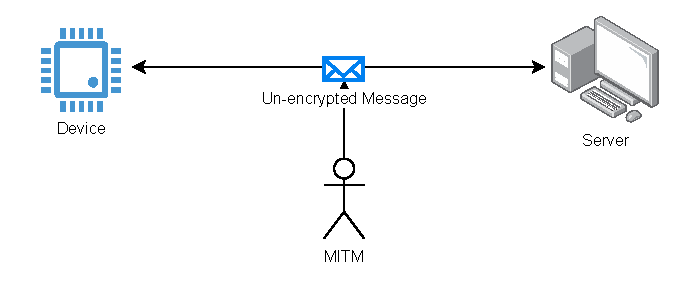
\includegraphics[width=0.7\linewidth]{images/MITM2.pdf}
    \caption{Tấn công MITM trong nghe lén dữ liệu}
    \label{fig:mitm1}
\end{figure}

\begin{figure}[h]
    \centering
    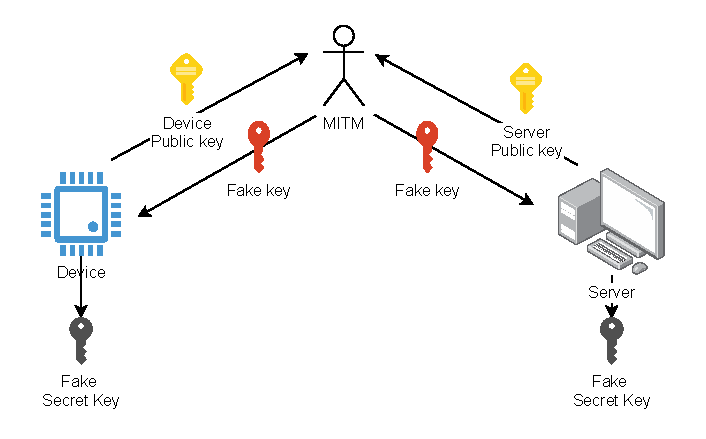
\includegraphics[width=0.7\linewidth]{images/MITM1.pdf}
    \caption{Tấn công MITM trong trao đổi khóa}
    \label{fig:mitm2}
\end{figure}

\subsection{Tấn công phát lại (Replay Attack)}
Tấn công phát lại (Replay Attack) là một dạng tấn công bảo mật trong đó kẻ tấn công chặn và ghi lại các gói tin hợp lệ từ quá trình giao tiếp giữa thiết bị IoT và máy chủ, sau đó gửi lại các gói tin này để lừa hệ thống thực hiện hành động không mong muốn, như cấp quyền truy cập trái phép hoặc thực thi lệnh giả mạo \cite{replay-attack}. Trong các hệ thống IoT, kẻ tấn công có thể ghi lại dữ liệu hợp lệ, chỉnh sửa nội dung, và gửi lại máy chủ, khiến máy chủ xử lý như gói tin hợp lệ, dẫn đến sai lệch thông tin (Hình \ref{fig:replay}). Trong các hệ thống IoT, đặc biệt là các ứng dụng thời gian thực như y tế hoặc giao thông thông minh, tấn công này đặc biệt nguy hiểm do dữ liệu sai lệch có thể gây hậu quả nghiêm trọng, ảnh hưởng trực tiếp đến an toàn và quyền lợi của người dùng.
\begin{figure}[h]
    \centering
    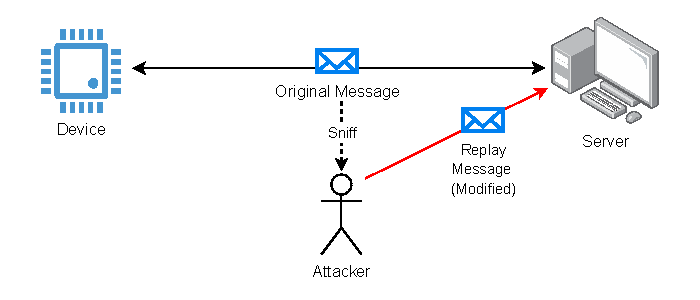
\includegraphics[width=0.7\linewidth]{images/replay.pdf}
    \caption{Minh họa cuộc tấn công phát lại}
    \label{fig:replay}
\end{figure}

\section{Khoảng trống nghiên cứu}
Dựa trên việc phân tích các ưu và nhược điểm của những nghiên cứu trước cũng như sự đa dạng và phức tạp của các hình thức tấn công vào hệ thống IoT, việc nghiên cứu và triển khai một kiến trúc bảo mật toàn diện là cần thiết và cũng là mục tiêu mà đề tài hướng đến. Bằng cách kết hợp các thuật toán mã hóa nhẹ, kiến trúc khung truyền độc lập kèm xác thực dữ liệu cùng với các phương pháp trao đổi khóa hiệu quả, đề tài hy vọng sẽ đóng góp một giải pháp có tính ứng dụng cao, đồng thời nâng cao tính bảo mật và khả năng mở rộng của hệ thống IoT trong thực tiễn.
% \section{Các phương pháp mã hóa nhẹ trong hệ thống IoT}
% (Phần này nên là lý do chọn Ascon)

% Trong các hệ thống IoT hạn chế tài nguyên, các thuật toán mã hóa truyền thống như AES hoặc RSA thường không phù hợp do yêu cầu tính toán và năng lượng cao, gây ra độ trễ lớn và tiêu tốn tài nguyên trên các thiết bị nhúng. Mã hóa nhẹ đã nổi lên như một giải pháp hiệu quả, cung cấp bảo mật mạnh mẽ với chi phí tính toán thấp. Các công trình nghiên cứu gần đây đã tập trung vào phát triển và đánh giá các thuật toán mã hóa nhẹ, chẳng hạn như Ascon và các biến thể của AES, nhằm đáp ứng nhu cầu của các ứng dụng IoT. Phần này xem xét các phương pháp mã hóa nhẹ nổi bật, làm rõ những hạn chế của chúng.

% Các công trình gần đây, chẳng hạn như bài báo Adaptive Lightweight Security for Performance Efficiency in Critical Healthcare Monitoring đã triển khai hệ thống IoT ứng dụng cho y tế đã so sánh 2 thuật toán mã hóa là Ascon-128 và AES-GCM-128 trên Raspberry Pi. Kết quả cho thấy Ascon-128 cho ra hiệu suất tốt hơn hoàn toàn so với AES-GCM-128 về mặt hiệu năng. Bài báo thực hiện so sánh tốc độ mã hóa của từng gói tin với kích thước khác nhau, Ascon cho ra hiệu suất cao với các gói tin có kích thước nhỏ, chẳng hạn với 8 byte dữ liệu, Ascon có hiệu suất gấp 8 lần so với AES và với 1024 byte, Ascon có hiệu suất gấp đôi. Với 2048 byte, Ascon vẫn cho ra hiệu suất tốt hơn dù mức độ chênh lệch không nhiều, hình \ref{fig:ascon-aes} được trích ra từ bài báo thể hiện hiệu suất của Ascon-128 so với phương pháp AES.

% \begin{figure}
%     \centering
%     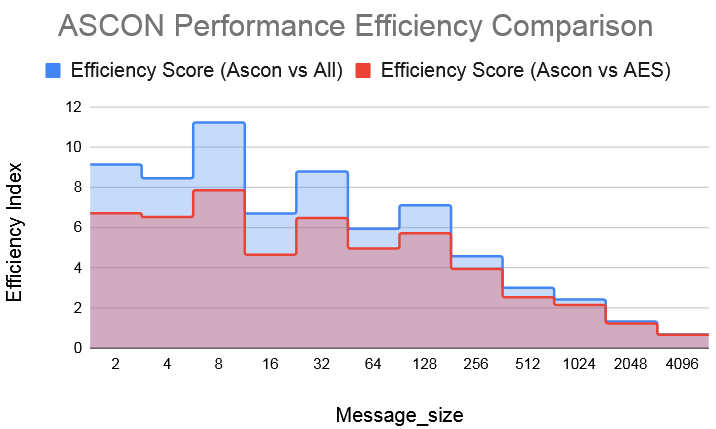
\includegraphics[width=0.8\linewidth]{ascon-aes.png}
%     \caption{Bảng so sánh hiệu năng giữa Ascon và AES được trích từ bài báo}
%     \label{fig:ascon-aes}
% \end{figure}

% Một nghiên cứu khác từ Dobraunig et al. (2021) trong bài giới thiệu Ascon v1.2 cũng nhấn mạnh hiệu suất cao của Ascon-128 khi thực hiện mã hóa dữ liệu có kích thước vừa và nhỏ so sánh với các thiết kế AES dùng native AES instruction trên Intel Skylake processors. 

% NIST cũng đã thực hiện đánh giá một số thuật toán mã hóa nhẹ ở vòng chung kết. Kết quả cho thấy Ascon là thuật toán có hiệu suất tốt nhất so với các thuật toán mã hóa nhẹ khác như Elephant, Grain-128aead hoặc Sparkle. Ascon cũng đã được NIST lựa chọn làm tiêu chuẩn mã hóa nhẹ chính thức vào năm 2023 dựa vào độ an toàn cao và hiệu suất vượt trội trên cả phần mềm lẫn phần cứng trong môi trường IoT giới hạn tài nguyên. NIST thực hiện đánh giá trên các nền tảng như 8-bit AVR, ARM Cortex-M0+/M3/M4, RISC-V, Xtensa LX6, v.v. Thời gian thực thi của Ascon nhanh hơn đáng kể so với chuẩn AES-GCM trên nRF52840. Trong các thử nghiệm benchmark độc lập, Ascon là một trong số ít thuật toán đạt hiệu suất cao và footprint nhỏ nhất, đặc biệt trên thiết bị nhúng có tài nguyên hạn chế.
% \section{Các công trình liên quan}

% Vấn đề về bảo mật trên các hệ thống IoT hạn chế tài nguyên được nghiên cứu rất nhiều trong thời gian gần đây. Các công trình nghiên cứu gần đây tập trung và nhiều biện pháp bảo mật khác nhau với nhiều kiến trúc khác nhau. Ở phần này sẽ liệt kê một số nghiên cứu và đánh giá các kiến trúc IoT đó để làm rõ những hạn chế của chúng cũng như nổi bật về nghiên cứu hiện tại của đề tài.

% \subsection{Các nghiên cứu liên quan đến ứng dụng AI trong bảo mật hệ thống IoT}

% \subsection{Các nghiên cứu liên quan đến ứng dụng mã hóa nhẹ trong đường truyền}

% \subsection{Các nghiên cứu liên quan đến trao đổi khóa mã hóa}



\chapter{Phương pháp đề xuất}
\label{Chapter3}

\section{Cơ sở lý thuyết}
Phần này trình bày chi tiết về cơ sở lý thuyết, các khái niệm cần thiết liên quan đến đề tài nghiên cứu.
\subsection{Kiến trúc IoT bốn lớp}
\label{sec:4layer}
Một kiến trúc IoT điển hình thường được tổ chức thành bốn lớp chính. Đầu tiên là lớp nhận thức (perceptual layer), bao gồm các thiết bị phần cứng như cảm biến và bộ điều khiển tại thiết bị biên, có nhiệm vụ thu thập và xử lý dữ liệu thô từ môi trường. Tiếp theo là lớp mạng (network layer), chịu trách nhiệm truyền tải dữ liệu giữa thiết bị và các nền tảng xử lý thông qua các giao thức kết nối có dây hoặc không dây. Dữ liệu sau đó được chuyển đến lớp xử lý dữ liệu (data processing layer), nơi thực hiện lưu trữ, phân tích và xử lý thông tin — thường được triển khai trên nền tảng điện toán đám mây. Cuối cùng, dữ liệu đã xử lý được hiển thị tới người dùng thông qua lớp ứng dụng (application layer), bao gồm các giao diện như ứng dụng di động, web hoặc phần mềm giám sát chuyên dụng.
\begin{figure}[h]
    \centering
    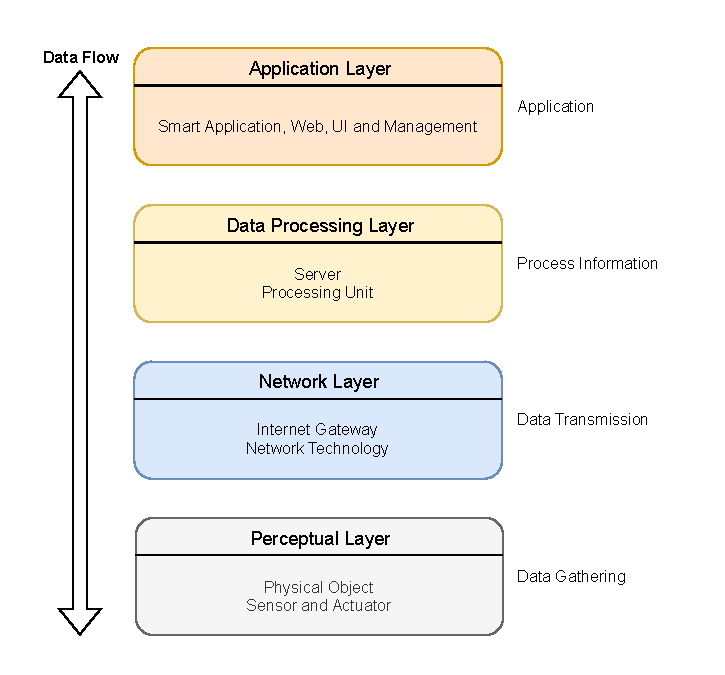
\includegraphics[width=0.75\linewidth]{images/4layer.pdf}
    \caption{Mô hình IoT 4 lớp}
    \label{fig:4layer}
\end{figure}
\subsubsection{Lớp nhận thức (Perceptual Layer)}
Đây là lớp đầu tiên của hệ thống, có nhiệm vụ thu thập dữ liệu từ nhiều nguồn khác nhau. Lớp này bao gồm các cảm biến được đặt trong môi trường nhằm thu thập dữ liệu về nhiệt độ, độ ẩm, ánh sáng và các dữ liệu vật lý khác. Các chuẩn giao tiếp có dây hoặc không dây thường được sử dụng để kết nối với lớp gateway ở trên.
\subsubsection{Lớp mạng (Network Layer)}
Lớp mạng thường được sử dụng như một gateway nhằm đảm bảo kết nối và truyền thông giữa các thiết bị IoT cũng như với mạng internet. Các công nghệ như Wi-Fi, Bluetooth, Zigbee, hoặc mạng di động (4G, 5G) được sử dụng, cùng với các cổng (gateway) như ESP32 sẽ được dùng để chuyển tiếp dữ liệu. Lớp này thường sử dụng các cơ chế mã hóa dữ liệu để đảm bảo an toàn trong quá trình truyền dữ liệu.
\subsubsection{Lớp xử lý dữ liệu (Data Processing Layer)}
Lớp xử lý dữ liệu thường là các máy chủ (server) trung gian có vai trò thu nhận, phân tích, và xử lý dữ liệu thô từ các thiết bị IoT. Các công cụ như hệ quản trị dữ liệu, nền tảng phân tích, hoặc thuật toán học máy được sử dụng để trích xuất thông tin giá trị. Lớp này cũng có vai trò xác định dữ liệu nhận từ các thiết bị có chính xác hay không, từ đó quyết định xem nên lưu trữ dữ liệu hay từ chối nhận dữ liệu từ bên ngoài.
\subsubsection{Lớp ứng dụng (Application Layer)}
Đây là lớp cao nhất, cung cấp giao diện thân thiện cho người dùng để tương tác với hệ thống IoT. Bao gồm các ứng dụng di động, web, và phần mềm trung gian (middleware) cho phép tích hợp và chia sẻ dữ liệu giữa các thiết bị.

\subsection{Giao thức MQTT}
Trong hệ thống IoT được xây dựng, giao thức được sử dụng để giao tiếp giữa gateway và máy chủ là giao thức MQTT (Message Queuing Telemetry Transport). Đây là một giao thức nhắn tin nhẹ, tối ưu cho các ứng dụng IoT, nơi yêu cầu truyền dữ liệu nhanh, gọn và tiêu tốn ít tài nguyên. Trong kiến trúc MQTT, Broker đóng vai trò là trung tâm phân phối thông điệp giữa các thiết bị, giúp chúng gửi và nhận thông điệp thông qua mô hình publish/subscribe. Khi một thiết bị publish một thông điệp đến một chủ đề (topic), Broker sẽ tiếp nhận và chuyển thông điệp đó đến mọi thiết bị đã subscribe topic tương ứng. Ngoài việc chuyển tiếp dữ liệu, Broker còn chịu trách nhiệm quản lý kết nối của các thiết bị, xử lý cơ chế giữ kết nối, và duy trì trạng thái phiên làm việc của client. 

\begin{figure}[h]
    \centering
    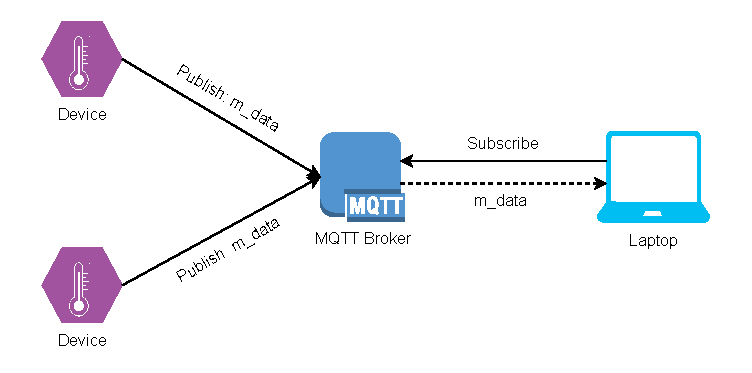
\includegraphics[width=0.85\linewidth]{mqtt.pdf}
    \caption{Giao thức MQTT}
    \label{fig:mqtt}
\end{figure}

\subsection{Mật mã hóa nhẹ ASCON-128a}
% \subsubsection{Giới thiệu về ASCON-128a}
Trong các hệ thống IoT hạn chế tài nguyên, việc sử dụng các thuật toán mã hóa truyền thống như AES hoặc RSA thường gặp nhiều bất cập do yêu cầu cao về năng lượng và khả năng tính toán. Điều này dẫn đến độ trễ lớn và tiêu tốn tài nguyên, ảnh hưởng đến hiệu quả hoạt động của các thiết bị nhúng. Trước thực trạng đó, mã hóa nhẹ (lightweight cryptography) đã được nghiên cứu và phát triển như một giải pháp tiềm năng, nhằm cung cấp mức độ bảo mật phù hợp với chi phí tính toán thấp.

% Gần đây, nhiều công trình nghiên cứu đã tập trung vào việc thiết kế và đánh giá các thuật toán mã hóa nhẹ, trong đó có Ascon và các biến thể tối ưu của AES, nhằm đáp ứng yêu cầu bảo mật cho các ứng dụng IoT. Nổi bật trong số đó là Ascon – thuật toán đã được Viện Tiêu chuẩn và Công nghệ Hoa Kỳ (NIST) lựa chọn làm tiêu chuẩn cho mã hóa nhẹ vào năm 2023 \cite{1984-TeX-Knuth}. Ascon là một thuật toán mã hóa xác thực kèm dữ liệu liên kết (Authenticated Encryption with Associated Data – AEAD), được thiết kế để đảm bảo mức độ bảo mật cao, hiệu suất xử lý tối ưu và cấu trúc đơn giản. Nhờ vào số lượng cổng logic thấp và khả năng chống chịu mạnh mẽ trước các tấn công mật mã học, Ascon trở thành một lựa chọn lý tưởng cho các thiết bị IoT có hạn chế về tài nguyên.

Các công trình gần đây, chẳng hạn như bài báo \cite{AESvsAscon} đã triển khai hệ thống IoT ứng dụng cho y tế đã so sánh 2 thuật toán mã hóa là Ascon-128 và AES-GCM-128 trên Raspberry Pi. Kết quả cho thấy Ascon-128 cho ra hiệu suất tốt hơn hoàn toàn so với AES-GCM-128 về mặt hiệu năng. Bài báo thực hiện so sánh tốc độ mã hóa của từng gói tin với kích thước khác nhau, Ascon cho ra hiệu suất cao với các gói tin có kích thước nhỏ, chẳng hạn với 8 byte dữ liệu, Ascon có hiệu suất gấp 8 lần so với AES và với 1024 byte, Ascon có hiệu suất gấp đôi. Với 2048 byte, Ascon vẫn cho ra hiệu suất tốt hơn dù mức độ chênh lệch không nhiều, hình \ref{fig:ascon-aes} được trích ra từ bài báo thể hiện hiệu suất của Ascon-128 so với phương pháp AES.

\begin{figure}[h]
    \centering
    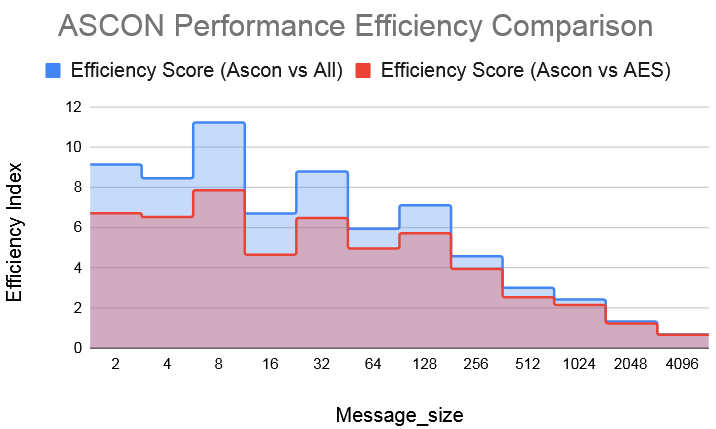
\includegraphics[width=0.7\linewidth]{ascon-aes.png}
    \caption{So sánh hiệu năng giữa Ascon và AES được trích từ bài báo}
    \label{fig:ascon-aes}
\end{figure}

Một nghiên cứu khác từ \cite{asconv1.2} trong bài giới thiệu Ascon v1.2 cũng nhấn mạnh hiệu suất cao của Ascon-128 khi thực hiện mã hóa dữ liệu có kích thước vừa và nhỏ so sánh với các thiết kế AES dùng native AES instruction trên Intel Skylake processors. 

Viện Tiêu chuẩn và Công nghệ Hoa Kỳ (NIST -- National Institute of Standards and Technology) cũng đã thực hiện đánh giá một số thuật toán mã hóa nhẹ ở vòng chung kết. Kết quả cho thấy Ascon là thuật toán có hiệu suất tốt nhất so với các thuật toán mã hóa nhẹ khác như Elephant, Grain-128aead hoặc Sparkle. Ascon cũng đã được NIST lựa chọn làm tiêu chuẩn mã hóa nhẹ chính thức vào năm 2023 dựa vào độ an toàn cao và hiệu suất vượt trội trên cả phần mềm lẫn phần cứng trong môi trường IoT giới hạn tài nguyên. NIST thực hiện đánh giá trên các nền tảng như 8-bit AVR, ARM Cortex-M0+/M3/M4, RISC-V, Xtensa LX6, v.v. Thời gian thực thi của Ascon nhanh hơn đáng kể so với chuẩn AES-GCM trên nRF52840. Trong các thử nghiệm benchmark độc lập, Ascon là một trong số ít thuật toán đạt hiệu suất cao và footprint nhỏ nhất, đặc biệt trên thiết bị nhúng có tài nguyên hạn chế.

\subsubsection{Thuật toán ASCON-128a}
ASCON là một bộ thuật toán mã hóa nhẹ bao gồm tập hợp các thiết kế mã hóa xác thực và một họ các hàm băm cùng hàm sinh đầu ra mở rộng. Ở đề tài này tập trung vào phần mã hóa xác thực trong triển khai hệ thống. Vì vậy, để đảm bảo tính ngắn gọn, chỉ có mã hóa xác thực được thảo luận trong phần này. ASCON sử dụng chế độ hoạt động dựa trên cấu trúc duplex, trong đó phép hoán vị 320-bit của ASCON được lặp lại thông qua một mạng hoán vị - thay thế (Substitution-Permutation Network - SPN) để thực hiện quá trình mã hóa hoặc giải mã dữ liệu. Quá trình này được thực hiện theo kiểu bit-slice, một đặc điểm giúp ASCON có khả năng mở rộng linh hoạt trên các nền tảng xử lý 8, 16, 32 và 64 bit, đồng thời vẫn đảm bảo tính "nhẹ" của thuật toán.

ASCON có hai biến thể chính phù hợp với độ dài khối dữ liệu cần mã hóa khác nhau: ASCON-128 và ASCON-128a. Trong các thuật toán mã hóa khối (block cipher), dữ liệu đầu vào được chia thành các khối có độ dài cố định. Trong đó, ASCON-128 sử dụng khối dữ liệu 64-bit và ASCON-128a sử dụng khối dữ liệu 128-bit. Các tập tham số tương ứng của từng biến thể ASCON được trình bày trong Bảng \ref{tab:ascon_parameter}. Như thể hiện trong bảng, điểm khác biệt chính giữa các biến thể là kích thước khối dữ liệu và số vòng lặp trong quá trình hoán vị.

Quy trình mã hóa của ASCON được mô tả trong Hình \ref{fig:ascon_process}, gồm bốn giai đoạn chính:
\begin{enumerate}
    \item Khởi tạo (Initialization)
    \item Xử lý dữ liệu liên kết (Associated Data Processing)
    \item Xử lý plaintext (Plaintext Processing)
    \item Kết thúc và tạo thẻ xác thực (Finalization for Tag Generation)
\end{enumerate}

\begin{figure}
    \centering
    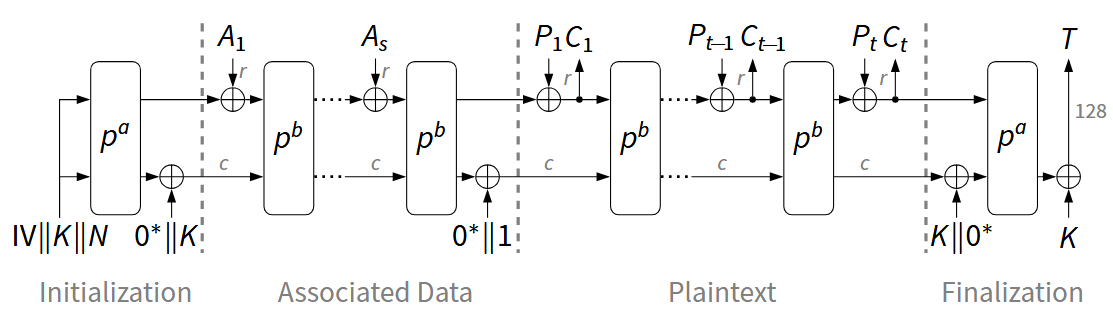
\includegraphics[width=0.9\linewidth]{ascon_process.png}
    \caption{Quá trình mã hóa của ASCON với dữ liệu liên kết}
    \label{fig:ascon_process}
\end{figure}

Trong suốt quá trình này, hai phép hoán vị 320-bit ký hiệu là $p^a$ và $p^b$ được sử dụng, trong đó $a$ và $b$ biểu thị số vòng lặp tương ứng. Các phép hoán vị này được biểu diễn theo dạng bit-slice, chia thành năm thanh ghi 64 bit, tạo thành trạng thái nội bộ gồm 5 word mỗi word có 64 bit.

Trong phiên bản ASCON đầy đủ với 12 vòng lặp, các phép hoán vị áp dụng lặp đi lặp lại quá trình biến đổi dựa trên mạng hoán vị - thay thế (SPN), bao gồm các bước: cộng hằng số vòng lặp (round constants), áp dụng lớp thay thế (substitution layer) và sử dụng lớp tuyến tính (linear layer) để khuếch tán dữ liệu trong trạng thái nội bộ.

Lớp thay thế (Substitution layer) sử dụng một hộp thế (S-box) gồm 5 bit có cấu trúc nhỏ gọn và tối ưu cho các hệ thống nhẹ, như minh họa trong Hình \ref{fig:s-box}. S-box được áp dụng song song 64 lần, nhằm cập nhật từng bit-slice trong trạng thái nội bộ. S-box 5 bit được thiết kế dựa trên login Boolean, cho phép triển khai hiệu quả trên cả hai nền tảng phần cứng ASIC và FPGA.

\begin{figure}
    \centering
    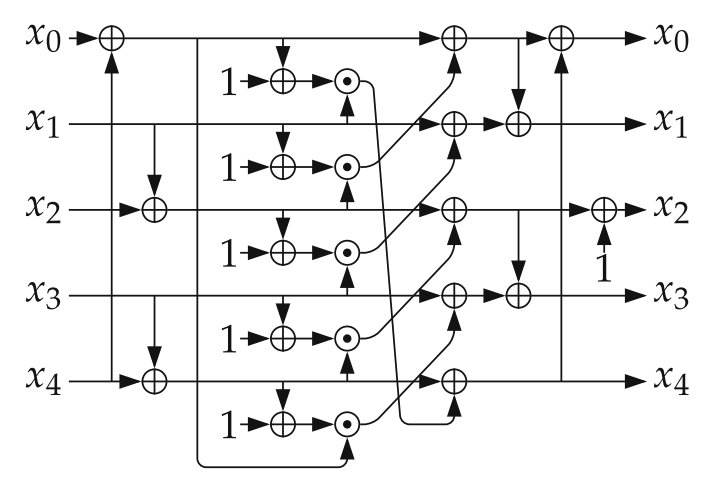
\includegraphics[width=0.6\linewidth]{s-box.png}
    \caption{Khối 5-bit S-box của ASCON}
    \label{fig:s-box}
\end{figure}

Lớp tuyến tính (Linear Layer) trong ASCON cập nhật mỗi word 64 bit trong trạng thái nội bộ bằng cách xoay (rotate) các thanh ghi với các giá trị dịch bit khác nhau, sau đó công theo modulo-2 (XOR) các giá trị đã được dịch.

Quá trình giải mã có một vài điểm khác biệt so với mã hóa. Thay vì xử lý plaintext, giải mã sử dụng hàm xử lý dữ liệu mã hóa (ciphertext processing), trong đó các khối plaintext được khôi phục bằng cách thực hiện phép XOR giữa khối plaintext và trạng thai hiện tại.

\begin{table}[ht]
\centering
\small
\caption{Bảng tham số cho ASCON}
\begin{tabular}{|p{3cm}|p{1.5cm}|p{1.5cm}|p{1.5cm}|p{2.8cm}|p{1cm}|p{1cm}|}
    \hline
    \multirow{2}{*}{Variants} & \multicolumn{4}{c|}{Bit size} & \multicolumn{2}{c|}{Rounds} \\
    \cline{2-7}
    & Key & Nonce & Tag & Data Block & $p^a$ & $p^b$ \\
    \hline
    ASCON-128 & 128 & 128 & 128 & 64 & 12 & 6 \\
    \hline
    ASCON-128a & 128 & 128 & 128 & 64 & 12 & 8 \\
    \hline
\end{tabular}
\label{tab:ascon_parameter}
\end{table}

\subsection{Thuật toán trao đổi khóa Elliptic Curve Diffie-Hellman}
\subsubsection{Đường cong Elliptic trên trường hữu hạn}
Một đường cong elliptic là một đường cong trơn (không có điểm nhọn hay tự cắt) được xác định bởi phương trình dạng
\[
    y^2 = x^3 + ax + b \pmod{p}
\]
trong đó $a$ và $b$ là các hằng số và $p$ là một số nguyên tố đại diện cho trường hữu hạn (finite field). Đường cong này có thể được diễn giải theo hình học và mang cấu trúc nhóm, cụ thể là một nhóm cộng với phép cộng điểm trên đường cong. Hình \ref{fig:curve} minh họa một đường cong elliptic với $a = -2$ và $b = 5$.

\begin{figure}[h]
    \centering
    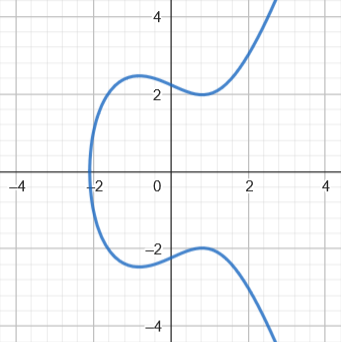
\includegraphics[width=0.4\linewidth]{curve.png}
    \caption{Đường cong elliptic $y^2 = x^3 - 2x + 5$}
    \label{fig:curve}
\end{figure}

Phép cộng hai điểm $P$ và $Q$ trên đường cong sẽ tạo ra một điểm thứ ba $R = P + Q$. Cách thực hiện là vẽ đường thẳng đi qua hai điểm $P$ và $Q$, tìm điểm giao thứ ba của đường thẳng đó với đường cong, sau đó phản xạ điểm này qua trục hoành (trục $x$) thể thu được điểm $R$.
\subsubsection{Trao đổi khóa Elliptic Curve Diffie-Hellman (ECDH)}
\label{sec:ecdh}
Elliptic Curve Diffie-Hellman (ECDH) là một thuật toán trao đổi khóa cho phép hai bên thiết lập một khóa bí mật chung qua kênh truyền thông không an toàn, dựa trên độ phức tạp tính toán của bài toán logarit rời rạc trên đường cong elliptic. Với hiệu suất cao và mức độ an toàn mạnh mẽ, ECDH được ứng dụng rộng rãi trong các giao thức mật mã. Cho \( G \) là điểm sinh (generator point) trên đường cong với bậc \( n \). Device và Gateway sẽ là hai thiết bị thực hiện trao đổi khóa với nhau, quá trình thực hiện ECDH được tóm tắt qua các bước sau:
\begin{enumerate}
    \item Device chọn khóa riêng (private key) \( d_A \in \mathbb{Z}_n \), và tính khóa công khai (public key) \( Q_A = d_A \cdot G \).
    \item Gateway thực hiện quá trình tương tự, chọn khóa riêng  \( d_B \in \mathbb{Z}_n \) và tính khóa công khai \( Q_B = d_B \cdot G \).
    \item Device và Gateway thực hiện trao đổi khóa công khai với nhau \( Q_A \) và \( Q_B \).
    \item Device tính khóa bí mật chung \( S_A = d_A \cdot Q_B \).
    \item Gateway tính khóa bí mật chung  \( S_B = d_B \cdot Q_A \).
    \item Do tính chất giao hoán của phép nhân điểm trên đường cong elliptic, \( S_A = S_B = d_A \cdot d_B \cdot G \), cả hai bên đạt được khóa bí mật chung \( S \).
\end{enumerate}
\begin{figure}[h]
    \centering
    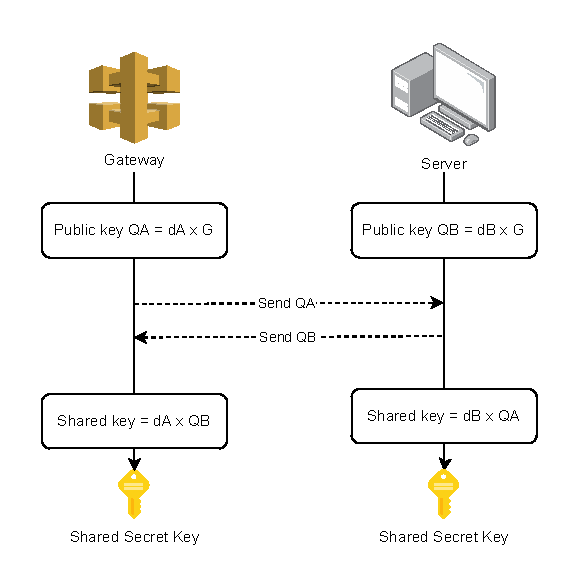
\includegraphics[width=0.65\linewidth]{images/keyexchange.pdf}
    \caption{Quá trình thực hiện trao đổi khóa ECDH}
    \label{fig:curve}
\end{figure}

Đề tài sử dụng đường cong \textit{sect163k1} trên trường hữu hạn $GF(2^{163})$, có phương trình sau:
\[
f(x) = x^{163} + x^7 + x^6 + x^3 + 1,
\]
được SECG (Standards for Efficient Cryptography Group) đề xuất nhờ khả năng tính toán hiệu quả trong họ đường cong Koblitz, giúp giảm chi phí xử lý tính toán. Với mức độ bảo mật tương đương 80-bit, đường cong này phù hợp cho các thiết bị IoT có tài nguyên hạn chế trong việc trao đổi khóa bảo mật \cite{secg}. Các tham số quan trọng bao gồm:

\[
a = 1, \quad b = 1, \quad h = 2,
\]
\[
n = \mathtt{04\; 00000000\; 00000000\; 00020108\; a2e0cc0d\; 99f8a5ef},
\]
Với điểm cơ sở \(G\):
\[
\begin{aligned}
G_x &= \mathtt{00000002\; fe13c053\; 7bbc11ac\; aa07d793} \\
    &\quad \mathtt{de4e6d5e\; 5c94eee8} \\
G_y &= \mathtt{00000002\; 89070fb0\; 5d38ff58\; 321f2e80} \\
    &\quad \mathtt{0536d538\; ccdaa3d9}
\end{aligned}
\]

ECDH đã được chứng minh có độ an toàn tương đương với thuật toán Diffie-Hellman truyền thống nhưng sử dụng các khóa có kích thước nhỏ hơn nhiều \cite{ecc-review} được trình bày ở Bảng \ref{tab:dh_ec_security}, điều này đặc biệt phù hợp với các thiết bị IoT có hạn chế về tài nguyên xử lý và bộ nhớ.

\begin{table}[h]
\centering
\small
\caption{Ratio of DH Security to EC Security at Different Security Levels}
\label{tab:dh_ec_security}
\begin{tabular}{|c|c|}
\hline
\textbf{Security Level (bits)} & \textbf{Ratio (DH : EC)} \\
\hline
80  & 3 : 1  \\
\hline
112 & 6 : 1  \\
\hline
128 & 10 : 1 \\
\hline
192 & 32 : 1 \\
\hline
256 & 64 : 1 \\
\hline
\end{tabular}
\end{table}

Mặc dù ECDH đòi hỏi chi phí tính toán cao hơn so với một số phương pháp đơn giản khác như sử dụng timestamp, bộ đếm (counter) hoặc khóa tĩnh, việc lựa chọn đường cong elliptic phù hợp sẽ giúp cân bằng giữa hiệu suất và bảo mật, từ đó đảm bảo hệ thống duy trì được mức độ an toàn trong thời gian dài.

\subsection{Hàm băm nhẹ ASCON}
\label{sec:ascon-hash}
Ascon sử dụng cấu trúc sponge duplex để cung cấp cả chức năng băm mật mã và mã hóa xác thực. Cấu trúc sponge là một phương thức vận hành, ánh xạ dữ liệu đầu vào có độ dài bất kỳ sang đầu ra có độ dài tuỳ chỉnh, thông qua một hàm hoán vị cố định và quy tắc đệm (padding). 
Cấu trúc này hoạt động trên một trạng thái hữu hạn, lặp lại việc áp dụng hàm hoán vị nội bộ, tổng quát hóa cả mã dòng với đầu vào cố định và hàm băm với đầu ra cố định. Sponge duplex là một biến thể của sponge, cho phép xen kẽ các khối đầu vào và đầu ra với tốc độ tương đương \cite{Ascon-Hash}.

Ascon-Hash là một hàm băm nhẹ dựa trên cấu trúc sponge, thực hiện hoán vị trên dữ liệu có kích thước bất kỳ để tạo ra giá trị băm 256-bit cố định, tối ưu cho các thiết bị nhúng. Sự tiêu chuẩn hóa của hàm băm Ascon trong NIST SP 800-232 và sự công nhận từ CAESAR làm tăng tính ứng dụng trong các hệ thống hạn chế tài nguyên, nơi hiệu suất và an ninh là ưu tiên hàng đầu. 
Theo kết quả đánh giá từ \cite{ascon-hash-2}, Ascon-Hash nhẹ hơn và tối ưu hơn cho phần cứng, đặc biệt trên các thiết bị như Arduino Due với ARM Cortex M3 so với các hàm băm truyền thống như SHA-256.
Hàm này sử dụng các thao tác đơn giản như XOR, dịch vòng (rotation), AND, NOT cùng với các hằng số để tối ưu hóa lớp thay thế (substitution layer), giúp tiết kiệm tài nguyên trên phần cứng \cite{Ascon-Hash}. Đặc tính nhẹ của Ascon-Hash cho phép triển khai hiệu quả trên các thiết bị IoT tài nguyên thấp, hỗ trợ nhiều bộ xử lý trong hệ thống với chi phí thấp.
Dựa trên cấu trúc sponge, Ascon-Hash vận hành qua ba giai đoạn chính: 
\begin{enumerate}
    \item Khởi tạo (Initialization): Trạng thái khởi tạo 320-bit của Ascon-Hash được xác định bởi hằng số \textit{IV}, trong đó chứa các thông số cấu hình của thuật toán gồm các giá trị như $k=0$, tốc độ xử lý dữ liệu $r$, số vòng lặp $a$ và $b$. Sau đó là độ dài đầu ra tối đa $h$ bit, đối với Ascon-Hash giá trị $h$ được khởi tạo là 0. Cuối cùng là một dãy 256-bit toàn số 0.
    \item Hấp thụ (Absorption): Dữ liệu đầu vào được chia thành các khối 64-bit, mỗi khối được XOR với trạng thái nội bộ 320-bit, sau đó áp dụng hàm hoán vị 12 vòng với các thao tác Addition, Rotation, XOR.
    \item Nén (Squeezing): Sau khi hấp thụ, trạng thái được xử lý thêm 12 vòng để tạo giá trị băm cuối cùng. 
\end{enumerate}

\begin{figure}[h]
    \centering
    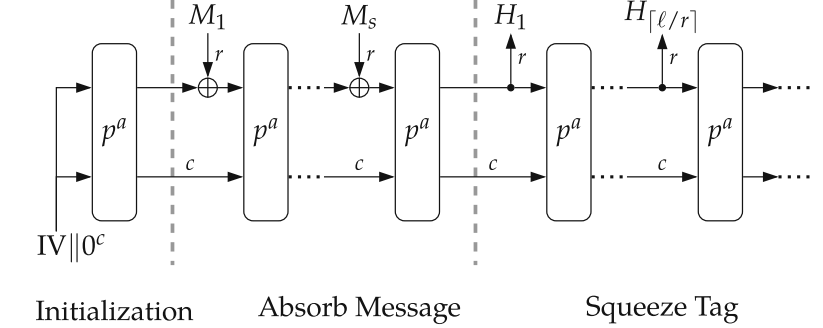
\includegraphics[width=0.8\linewidth]{ascon_hash.png}
    \caption{Chế độ băm Ascon-Hash}
    \label{fig:asconhash}
\end{figure}

Ở mỗi phiên, khóa bí mật được tạo ra sau khi thực hiện trao đổi khóa ECDH sẽ được đưa vào hàm Ascon-Hash nhằm tạo ra khóa phiên cho mã hóa và giải mã dữ liệu.
% \subsection{Kiến trúc khung truyền}
% (có thể thêm để nói về kiến trúc khung truyền)

\section{Phương pháp thực hiện}
\label{sec:phuongphap}
\subsection{Tổng quan hệ thống IoT}
Mô hình IoT được triển khai dựa trên kiến trúc IoT bốn lớp như trình bày ở phần \ref{sec:4layer}. Ở lớp nhận thức, vi điều khiển STM32F411VET6 được sử dụng để thu thập dữ liệu từ cảm biến. Dữ liệu sau đó được truyền tới lớp xử lý dữ liệu thông qua ESP32, thiết bị đóng vai trò như một gateway trung gian. Giao tiếp giữa STM32 và ESP32 được thực hiện thông qua giao thức UART. Trên máy chủ Linux, các thành phần được triển khai bao gồm MQTT Broker và Backend chịu trách nhiệm tiếp nhận dữ liệu từ gateway, xử lý và phân giải các gói tin, kiểm tra tính hợp lệ của gói tin. Hình \ref{fig:realsystem} trình bày mô hình tổng quan của hệ thống. Phần dưới đây sẽ trình bày từng thành phần trong hệ thống, các khái niệm về khung truyền được đề cập tới sẽ trình bày chi tiết ở các phần \ref{sec:tongquan} và \ref{sec:frame}.

 % MQTT Broker đảm nhiệm việc thiết lập và duy trì kênh giao tiếp theo giao thức MQTT giữa gateway và máy chủ. Trong khi đó, Backend thực hiện xử lý nội dung dữ liệu, giải mã thông tin và quản lý cơ chế trao đổi khóa bảo mật với gateway. Những gói tin không hợp lệ sẽ được Backend Server phát hiện và từ chối ngay lập tức nhằm đảm bảo tính ổn định và an toàn cho người dùng cuối. 

\begin{figure}[h]
    \centering
    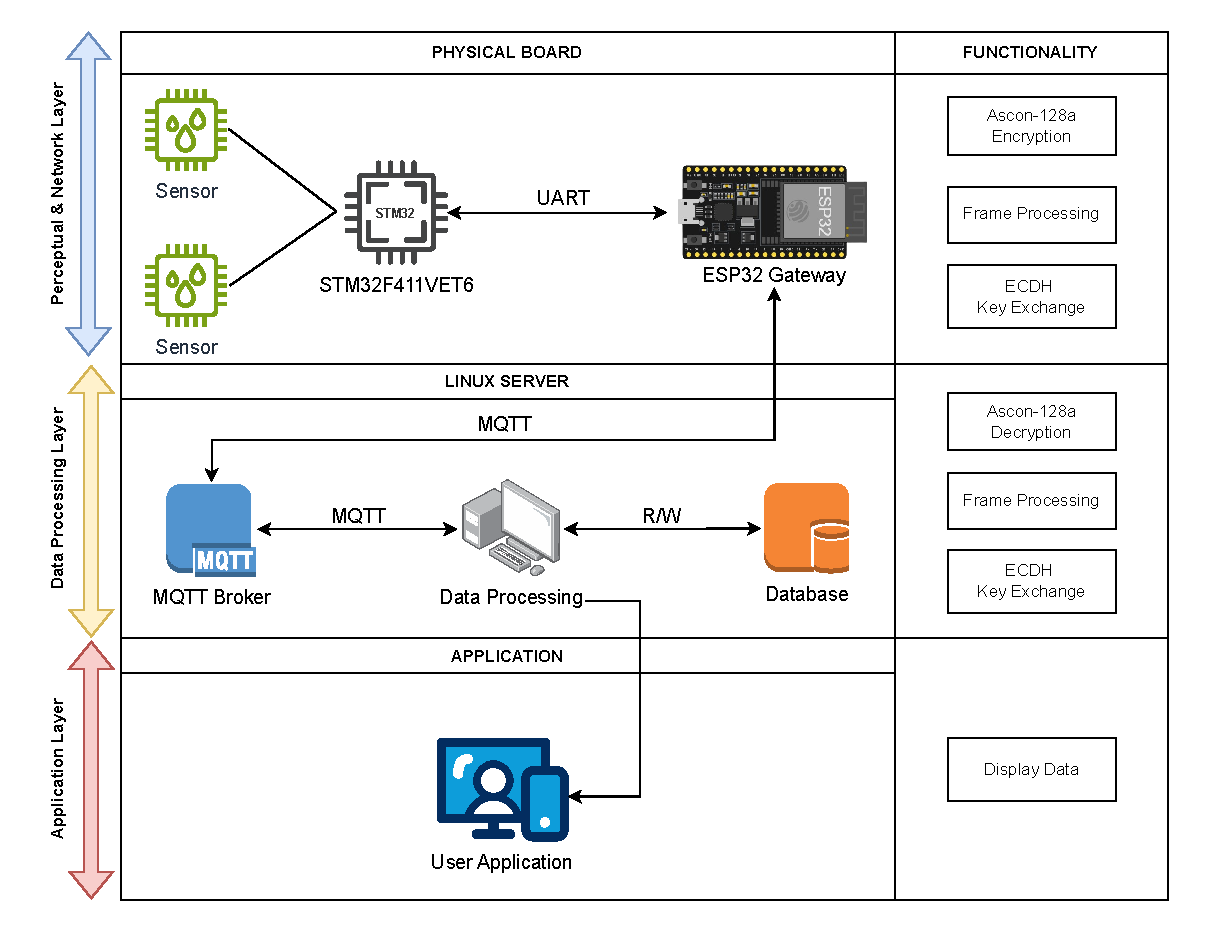
\includegraphics[width=1\linewidth]{realsystem.pdf}
    \caption{Mô hình tổng quan hệ thống}
    \label{fig:realsystem}
\end{figure}

\subsubsection{STM32F411VET6 MCU}
Vi điều khiển STM32F411VET6 được phát triển dựa trên bộ công cụ STM32CubeIDE kết hợp với STM32CubeMX. Trong kiến trúc hệ thống đề xuất, STM32 được sử dụng ở lớp nhận thức nhằm thu thập dữ liệu xung quanh thông qua các cảm biến được kết nối. Sau khi dữ liệu được thu thập, STM32 sẽ tiến hành mã hóa dữ liệu bằng thuật toán mã hóa nhẹ Ascon-128a. Tiếp theo, STM32 sẽ cấu trúc dữ liệu đã mã hóa thành khung truyền, và gửi đến lớp mạng để tiếp tục xử lý. Trước mỗi lần mã hóa, STM32 sẽ tạo các khóa phiên bằng cách sử dụng hàm băm Ascon Hash, đảm bảo mỗi khối dữ liệu sẽ sử dụng một khóa mã hóa khác nhau nhằm tăng cường tính bảo mật (kỹ thuật tạo khóa phiên sẽ được trình bày ở phần \ref{sec:key}). Thứ tự khóa phiên sẽ được STM32 đồng bộ liên tục cùng với máy chủ để đảm bảo quá trình mã hóa - giải mã được thực hiện chính xác.

\subsubsection{ESP32 Gateway}
ESP32 đóng vai trò như một IoT gateway tại lớp mạng trong mô hình IoT bốn lớp. Đây là thành phần quan trọng và có mức độ phức tạp cao nhất trong quá trình triển khai hệ thống. ESP32 đóng vai trò trung gian, thực hiện chuyển tiếp dữ liệu giữa lớp nhận thức (các thiết bị cảm biến sử dụng vi điều khiển STM32) sử dụng giao thức UART và lớp xử lý dữ liệu (máy chủ) sử dụng giao thức MQTT. Mọi khung truyền được gửi đến gateway sẽ được phân giải và kiểm tra tính toàn vẹn trước khi chuyển tiếp giữa các lớp, đảm bảo rằng chỉ dữ liệu hợp lệ mới được truyền đi. ESP32 là thiết bị thực hiện việc cấu trúc nhiều bộ khung truyền nhất trong hệ thống với tổng cộng năm bộ khung được định nghĩa và sử dụng tại đây. ESP32 cũng là nơi bắt đầu quá trình trao đổi khóa bí mật chung, khi khóa bí mật chung hết hạn hoặc có dấu hiện bị lộ, ESP32 sẽ tiến hành yêu cầu quá trình trao đổi khóa bí mật chung với máy chủ. Đặc biệt, cơ chế \textit{safe counter} (trình bày ở phần \ref{sec:safe_counter}) cũng được triển khai trong ESP32, đây là một trong những cơ chế quan trọng giúp tăng tính bảo mật của hệ thống. Nhìn chung, đây là thành phần rất quan trọng, không chỉ đảm nhận chức năng giao tiếp mà còn thực hiện nhiều nhiệm vụ bảo mật quan trọng, góp phần đảm bảo sự ổn định và an toàn của toàn bộ kiến trúc IoT.

\subsubsection{Hệ thống máy chủ}
Máy chủ đóng vai trò trung tâm trong hệ thống IoT nằm ở lớp xử lý dữ liệu trong kiến trúc IoT bốn lớp, chịu trách nhiệm tiếp nhận dữ liệu từ gateway, xử lý và phân giải các gói tin, kiểm tra tính hợp lệ của gói tin, sau đó cung cấp thông tin đến người dùng cuối. Trong hệ thống này, thành phần máy chủ được triển khai trên máy tính sử dụng hệ điều hành Linux. Trên máy chủ bao gồm hai thành phần chính là hệ thống Backend và MQTT Broker. 

Đầu tiên là thành phần MQTT Broker, được triển khai trên máy chủ sử dụng Aedes. Đây là một MQTT Broker nhẹ được phát triển bằng ngôn ngữ JavaScript, phù hợp để tích hợp với hệ thống Node.js. Việc lựa chọn tự triển khai MQTT Broker trên máy chủ thay vì sử dụng các dịch vụ MQTT Broker public xuất phát từ hai lý do chính. Trước hết, độ trễ khi sử dụng Broker public thường cao hơn nhiều do lượng lớn người dùng chia sẻ cùng một hạ tầng dẫn đến tình trạng tắc nghẽn hoặc chậm phản hồi. Ngược lại, triển khai Broker riêng giúp tối ưu tốc độ giao tiếp nhờ kiểm soát hoàn toàn tài nguyên và môi trường mạng. Thứ hai, tự cấu hình Broker cho phép tích hợp thêm các tính năng bảo mật quan trọng như xác thực người dùng, phân quyền truy cập theo topic, và giới hạn quyền publish/subscribe chỉ dành cho các thiết bị đáng tin cậy. Điều này nâng cao tính bảo mật và khả năng kiểm soát trong hệ thống, đặc biệt quan trọng đối với các ứng dụng IoT yêu cầu tính riêng tư và độ tin cậy cao. 

Hệ thống Backend chính là nơi tiếp nhận dữ liệu từ gateway và tiến hành xử lý dữ liệu. Khi nhận được khung truyền từ gateway, Backend sẽ tiến hành phân giải để kiểm tra. Đối với các gói tin không hợp lệ, Backend có khả năng từ chối ngay lập tức để không ảnh hưởng đến người dùng. Trong kiến trúc hệ thống này, Backend được cấu hình để thực hiện một số chức năng quan trọng liên quan đến bảo mật và xử lý dữ liệu. Thuật toán trao đổi khóa ECDH được sử dụng để thiết lập khóa chung bí mật giữa gateway, trong khi thuật toán Ascon-128a đảm nhiệm việc giải mã và xác thực dữ liệu nhận được. Ngoài ra, máy chủ còn sử dụng hàm băm Ascon Hash nhằm tạo ra khóa phiên cho quá trình giải mã. Cơ chế \textit{safe counter} cũng được triển khai tại đây nhằm tăng tính bảo mật của hệ thống. Hệ thống Backend được triển khai trên nền tảng Node.js, với JavaScript là ngôn ngữ lập trình chính, giúp đảm bảo khả năng mở rộng, xử lý bất đồng bộ hiệu quả và dễ dàng tích hợp với các thành phần khác trong hệ thống.


\subsection{Mô hình giao tiếp của hệ thống}
\label{sec:tongquan}
Hệ thống IoT được chia thành ba quá trình giao tiếp: khởi tạo, trao đổi khóa và truyền dữ liệu. Tất cả dữ liệu trên đường truyền được đảm bảo mã hóa và xác thực. Ngoài ra, tất cả quá trình truyền sẽ được đóng gói thành các khung truyền được cấu hình độc nhất cho mỗi gói tin trình bày ở phần \ref{sec:4layer}. Hình \ref{fig:system} minh họa mô hình giao tiếp của hệ thống.

\begin{figure}[h]
    \centering
    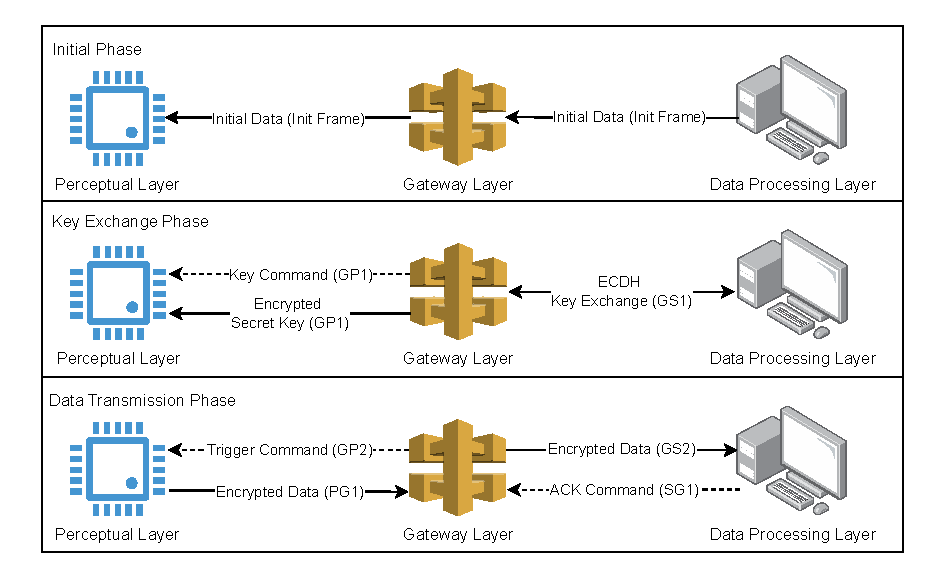
\includegraphics[width=0.85\linewidth]{images/system.pdf}
    \caption{Mô hình giao tiếp của hệ thống}
    \label{fig:system}
\end{figure}

Mỗi khi thiết bị khởi động hoặc reboot, phiên khởi tạo sẽ được kích hoạt. Trong phiên này, máy chủ sẽ truyền các thông tin đồng bộ, bao gồm \textit{safe counter} và \textit{key index} đến thiết bị. Những dữ liệu này đóng vai trò thiết yếu trong việc đảm bảo đồng bộ hóa, khôi phục trạng thái hệ thống, và duy trì tính toàn vẹn của quá trình truyền dữ liệu. Phần \ref{sec:safe_counter} sẽ trình bày ý nghĩa của \textit{safe counter} và phần \ref{sec:key} sẽ trình bày chi tiết về cách hoạt động của \textit{key index}.

Trong quá trình trao đổi khóa, gateway và máy chủ sẽ trao đổi khóa với nhau bằng thuật toán ECDH để có thể tạo ra hai khóa bí mật sử dụng cho mã hóa và giải mã. Dữ liệu sẽ được mã hóa ngay tại lớp nhận thức, vì vậy sau khi sinh thành công khóa bí mật, gateway sẽ chuyển khóa này đến lớp giao thức để tiến hành mã hóa dữ liệu. Để tránh lộ khóa bí mật, gateway tiến hành mã hóa khóa này bằng một khóa chia sẻ trước (pre-shared key) trước khi truyền xuống lớp nhận thức. Tại lớp nhận thức, khóa được giải mã và sử dụng cho quá trình mã hóa dữ liệu. Cơ chế này giúp đảm bảo khóa bí mật không bị lộ hoặc đánh chặn trong quá trình trao đổi khóa, qua đó tăng cường tính an toàn cho hệ thống.

Phần lớn thời gian STM32 tại lớp nhận thức sẽ ở trong chế độ ngủ (Sleep Mode) để có thể tiết kiệm năng lượng. Vì vậy, để bắt đầu quá trình truyền dữ liệu, gateway trước tiên sẽ gửi một tín hiệu kích hoạt (trigger signal) cho lớp nhận thức. Khi nhận được tín hiệu, lớp nhận thức sẽ thoát khỏi sleep mode để tiến hành thu thập và mã hóa dữ liệu thu được bằng các khóa phiên được băm từ khóa bí mật (như trình bày ở phần \ref{sec:ascon-hash}) và gửi lên cho gateway. Gateway sẽ tiếp tục chuyển tiếp dữ liệu này lên cho máy chủ để xử lý. Nếu máy chủ có thể giải mã dữ liệu thành công, máy chủ sẽ gửi lại cho gateway một tín hiệu ACK nhằm thông báo phiên truyền dữ liệu thành công và tiếp tục bắt đầu phiên truyền mới. Trong trường hợp gateway không nhận được tín hiệu ACK từ máy chủ sau một khoảng thời gian nhất định (timeout), điều này có nghĩa dữ liệu đã không được truyền thành công hoặc giải mã không thành công, gateway sẽ gửi một gói tin thông báo cho STM32 ở lớp nhận thức để STM32 đồng bộ lại dữ liệu và bắt đầu lại phiên truyền. Hình \ref{fig:trans-sys} mô tả chi tiết toàn bộ quá trình giao tiếp của hệ thống bao gồm các khung truyền sẽ được trình bày chi tiết trong phần \ref{sec:frame}.

\begin{figure}[htbp]
    \centering
    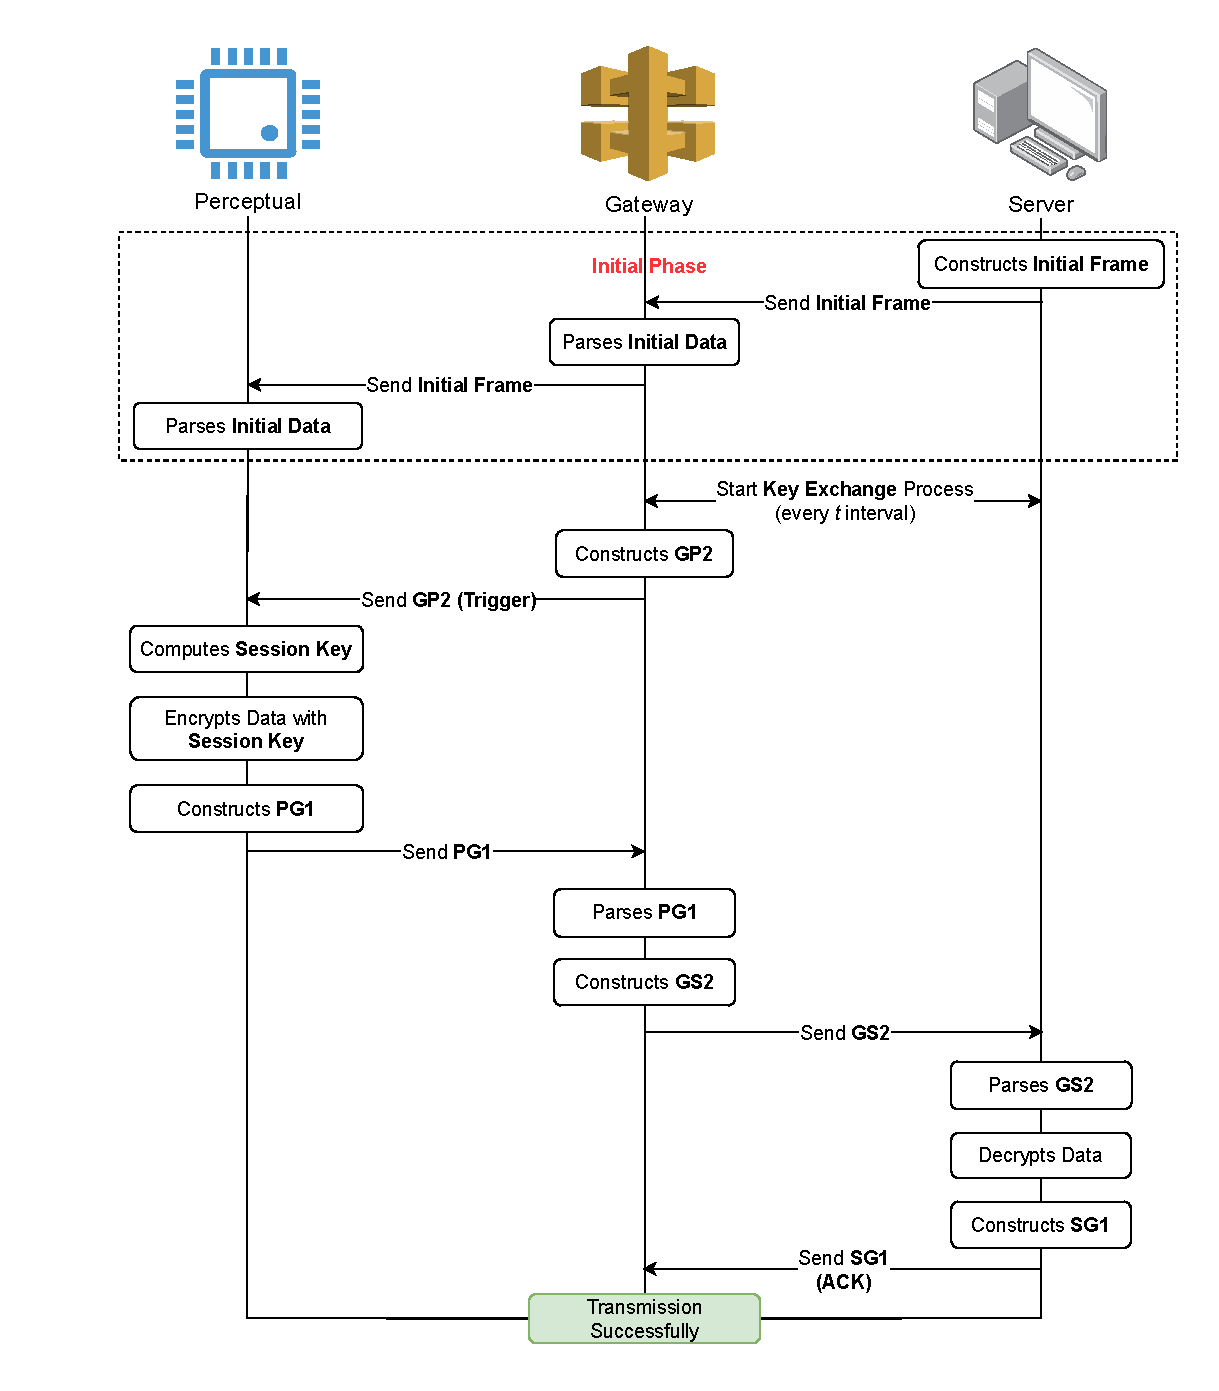
\includegraphics[width=1\linewidth]{trans-sys.pdf}
    \caption{Luồng hoạt động của hệ thống}
    \label{fig:trans-sys}
\end{figure}

\subsection{Phương pháp tạo khóa phiên từ khóa bí mật sử dụng trong mã hóa và giải mã dữ liệu}
\label{sec:key}
Để đảm bảo an toàn cho hệ thống IoT, việc thiết kế một phương thức trao đổi khóa bí mật an toàn là vô cùng cần thiết. Khóa bí mật này đóng vai trò quan trọng trong việc mã hóa và giải mã dữ liệu, góp phần bảo vệ tính toàn vẹn và bảo mật thông tin truyền tải. Nếu hệ thống IoT sử dụng phương pháp trao đổi khóa, tạo khóa kém an toàn hoặc dựa trên khóa tĩnh được cài đặt một lần duy nhất, nguy cơ lộ khóa hoặc bị tấn công brute-force với khóa có độ dài bit bảo mật thấp sẽ tăng lên đáng kể. 

Như đã trình bày trong phần \ref{sec:ecdh}, nhược điểm lớn của ECDH chính là chi phí tính toán lớn, điều này có thể ảnh hưởng đến độ trễ của hệ thống. Vì vậy, để đảm bảo khóa luôn được làm mới và hạn chế quá trình trao đổi khóa liên tục, đề tài đề xuất một phương pháp tạo khóa phiên dựa trên khóa bí mật để giải quyết vấn đề trên. Trong đề tài này, thuật toán trao đổi khóa Elliptic Curve Diffie-Hellman (ECDH) được áp dụng nhằm thiết lập khóa bí mật trên kênh truyền không an toàn, đồng thời kết hợp với hàm băm nhẹ ASCON để sinh các khóa phiên (session key) phục vụ cho quá trình mã hóa, giải mã dữ liệu. Hình \ref{fig:skey} thể hiện quá trình tạo khóa phiên đề xuất.

\begin{figure}[h]
    \centering
    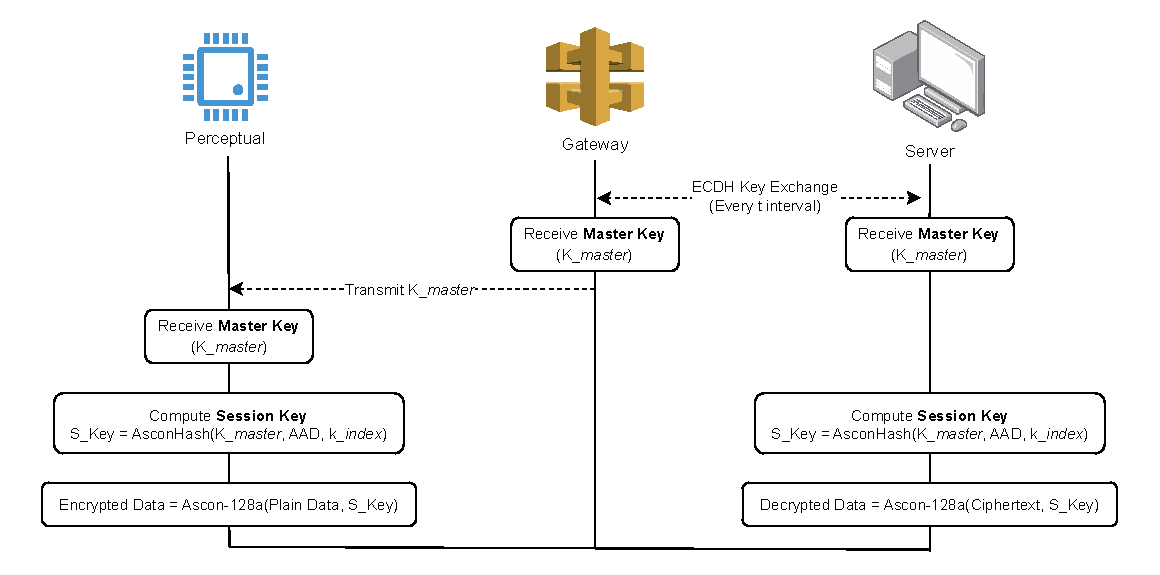
\includegraphics[width=1\linewidth]{skey.pdf}
    \caption{Quy trình tạo khóa phiên}
    \label{fig:skey}
\end{figure}

Sau khi hoàn thành trao đổi khóa như đã trình bày ở phần \ref{sec:ecdh}, gateway và server sẽ tạo ra hai khóa bí mật, ở phần này sẽ gọi là Master Key ($K_{master}$). Thời gian giữa mỗi lần trao đổi $K_{master}$ được gọi là $t$, được cấu hình tùy vào yêu cầu bảo mật của hệ thống, $t$ càng nhỏ thì quá trình trao đổi $K_{master}$ sẽ diễn ra với tần suất nhiều hơn nhưng bù lại sẽ tốn nhiều tài nguyên và thời gian cho việc trao đổi khóa. Và như đã trình bày ở phần \ref{sec:tongquan}, $K_{master}$ sẽ được truyền xuống lớp nhận thức để phục vụ quá trình mã hóa.  Trước khi lớp nhận thức mã hóa dữ liệu, khóa phiên sẽ được tạo ra bằng hàm băm ASCON. Đầu vào của hàm băm ASCON là sự kết hợp của các thành phần sau: $K_{master}$, $AAD$ và $k_{index}$. Trong đó $AAD$ là Associated Data được sử dụng trong mã hóa xác thực Ascon-128a và $k_{index}$ chính là thứ tự của khóa hiện tại và tăng dần sau mỗi phiên. 
\[
input = K_{master} || \text{AAD} ||k_{index}
\]
Kết quả của hàm băm với đầu vào $input$ sẽ cho ra khóa phiên và sử dụng cho việc mã hóa dữ liệu. Phía server cũng sẽ sử dụng quá trình tương tự để tạo khóa phiên cho việc giải mã. Với $k_{index}$ thay đổi liên tục, khóa phiên sinh ra cũng sẽ thay đổi liên tục, đảm bảo việc dò khóa sẽ rất phức tạp. 

\[
    K_{session} = \text{AsconHash}(K_{master} || \text{AAD} ||k_{index})
\]

\subsection{Kiến trúc khung truyền giao tiếp giữa các lớp trong hệ thống IoT}
\label{sec:frame}
Phần này sẽ trình bày chi tiết về kiến trúc khung truyền được sử dụng trong hệ thống, được sử dụng trong giao tiếp giữa các lớp như minh họa ở hình \ref{fig:system}. Tất cả các khung đều có các trường chuẩn được trình
bày trong hình \ref{fig:gframe}.
\begin{figure}[H]
    \centering
    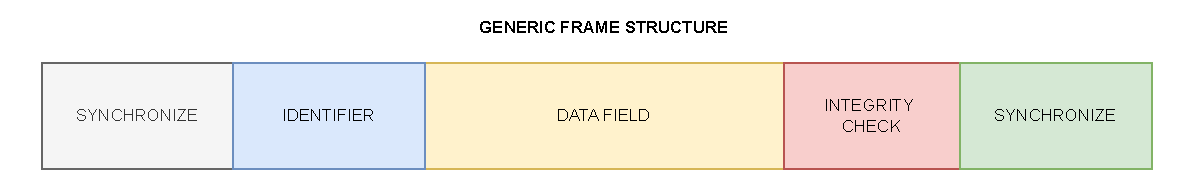
\includegraphics[width=0.9\linewidth]{gframe.pdf}
    \caption{Cấu trúc khung truyền tổng quát}
    \label{fig:gframe}
\end{figure}

Khung truyền bắt đầu và kết thúc bằng các trường đồng bộ, bao gồm 2 byte Start of Frame (SOF) đánh dấu bắt đầu khung và 2 byte End of Frame (EOF) đánh dấu kết thúc. Các trường này giúp thiết bị nhận xác định ranh giới hợp lệ của một khung dữ liệu.
Tiếp theo là trường định danh thiết bị (Identifier) dài 4 byte, được sử dụng để định danh duy nhất thiết bị gửi hoặc nhận.
Trường dữ liệu (Data) mang thông tin chính cần truyền đi. Trường này cũng có thể bao gồm các tham số liên quan đến quá trình mã hóa và giải mã, chẳng hạn như nonce hoặc associated data.
Cuối cùng là trường kiểm tra toàn vẹn (Integrity Check), đảm bảo rằng dữ liệu nhận được không bị lỗi hoặc bị thay đổi trong quá trình truyền. Trường này có thể chứa mã xác thực (ví dụ: Auth Tag từ các hàm mã hóa xác thực) hoặc mã kiểm lỗi như CRC, tùy theo loại khung.

Để dễ hiểu, mỗi khung truyền sẽ được đặt tên dựa trên lớp nguồn và lớp đích, ngoại trừ khung truyền khởi tạo; ví dụ, một khung truyền từ gateway đến máy chủ (server) sẽ được ký hiệu là GS (Gateway-Server). Đối với dữ liệu liên quan (Associated Data - $AAD$), ở phần này sẽ sử dụng hai $AAD$ bao gồm $AAD_{data}$ và $AAD_{key}$. Trong đó, $AAD_{data}$ được tính toán mỗi phiên truyền dữ liệu và $AAD_{key}$ được cấu hình sẵn và sử dụng trong các phiên trao đổi khóa giữa gateway và máy chủ. Phần này sẽ chia các khung truyền thành ba nhóm chính: khung truyền khởi tạo, khung truyền trong giao tiếp giữa lớp nhận thức và gateway, khung truyền trong giao tiếp giữa gateway và máy chủ.
\subsubsection{Khung truyền khởi tạo}
Khung truyền khởi tạo này có kiến trúc rất đơn giản, chỉ bao gồm các trường chuẩn như trình bày ở phần trên. Khung truyền này chứa các dữ liệu cần thiết giúp máy chủ đồng bộ giao tiếp với thiết bị. Trường dữ liệu của khung khởi tạo bao gồm 2-byte \textit{safe counter} và 2-byte \textit{key index} hỗ trợ thiết lập trạng thái ban đầu và đảm bảo tính toàn vẹn hệ thống. Trong suốt vòng đời hoạt động, khung khởi tạo chỉ được kích hoạt một lần duy nhất ngay sau khi thiết bị khởi động lại.
\begin{figure}[H]
    \centering
    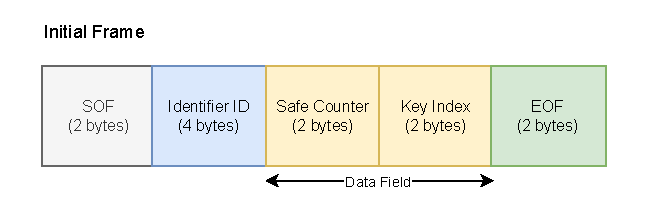
\includegraphics[width=0.6\linewidth]{init-frame.pdf}
    \caption{Khung truyền khởi tạo}
    \label{fig:init-frame}
\end{figure}
\subsubsection{Khung truyền trong giao tiếp giữa lớp nhận thức và lớp mạng}
Phần này mô tả chi tiết cấu trúc khung truyền trong quá trình giao tiếp giữa lớp nhận thức và lớp mạng. Hình \ref{fig:gp} minh họa khung truyền được sử dụng khi dữ liệu được gửi từ lớp mạng xuống lớp nhận thức, ký hiệu là GP. Trong khung truyền này, một trường 1 byte có tên là \textit{packet type} được thêm vào để xác định loại dữ liệu đang được truyền. Hai loại khung chính được định nghĩa: một dành cho việc truyền khóa bí mật (GP1), và một dành cho truyền tín hiệu kích hoạt (GP2). 

Với khung truyền GP2, trường dữ liệu của khung sẽ chỉ chứa 16-byte $AAD_{data}$ dùng cho mã hóa dữ liệu, tức là, lớp nhận thức sẽ sử dụng 16-byte $AAD_{data}$ này cho việc mã hóa dữ liệu trước khi truyền đi. Ngoài ra, 2-byte CRC được thêm vào để kiểm tra lỗi trong quá trình truyền. Các trường chuẩn của GP2 vẫn được giữ nguyên.

Khung truyền GP1 sẽ có sự phức tạp hơn do đây là khung đảm nhận vai trò truyền khóa bí mật xuống lớp nhận thức, vì đây là dữ liệu nhạy cảm nên một số trường bổ sung được thêm vào. Trường dữ liệu của GP1 sẽ bao gồm 16-byte \textit{Nonce} và $AAD_{data}$, $AAD_{data}$ vẫn sẽ được sử dụng trong mã hóa dữ liệu trước khi truyền. \textit{Nonce} và $AAD_{key}$ là hai dữ liệu quan trọng để lớp nhận thức có thể giải mã khóa bí mật (khóa bí mật sẽ được mã hóa bởi gateway trước khi truyền xuống lớp nhận thức như trình bày ở phần \ref{sec:tongquan}) với $AAD_{key}$ đã được cấu hình tĩnh trước cho cả lớp giao thức và gateway. Tiếp theo đó, sẽ là 1-byte \textit{secret key length} và phần tải chứa khóa bí mật đã được mã hóa, trong đó 1-byte \textit{secret key length} biểu thị độ dài của khóa bí mật. Một trường quan trọng được bổ sung vào khung GP1 đó chính là 16-byte \textit{authentication tag} (Auth Tag), được sinh ra trong quá trình mã hóa khóa bí mật với Ascon-128a. Phần \ref{sec:mitm} đã trình bày việc tấn công Man-in-the-Middle có thể đánh tráo khóa trên đường truyền, vì vậy Auth Tag được thêm vào để đảm bảo dữ liệu được xác thực, nếu việc tính toán Auth Tag sai và không trùng khớp, lớp nhận thức sẽ ngay lập tức từ chối khóa bí mật này, tránh việc sử dụng khóa giả mạo cho việc mã hóa và giải mã.

Về cách tính $AAD_{data}$ trong GP1 và GP2, $AAD_{data}$ được ghép từ một số trường dữ liệu trong GS2 (trình bày ở phần \ref{sec:gs}). Vì thế, $AAD_{data}$ sẽ được tính như sau:
\[
\text{$AAD_{data}$} = \text{SOF}_{2} \, || \, \text{Identifier ID}_{4} \, || \, \text{Sequence Number}_{4} \, || \, \text{Nonce}_{4} \, || \, \text{EOF}_{2}
\]

\begin{figure}[h]
    \centering
    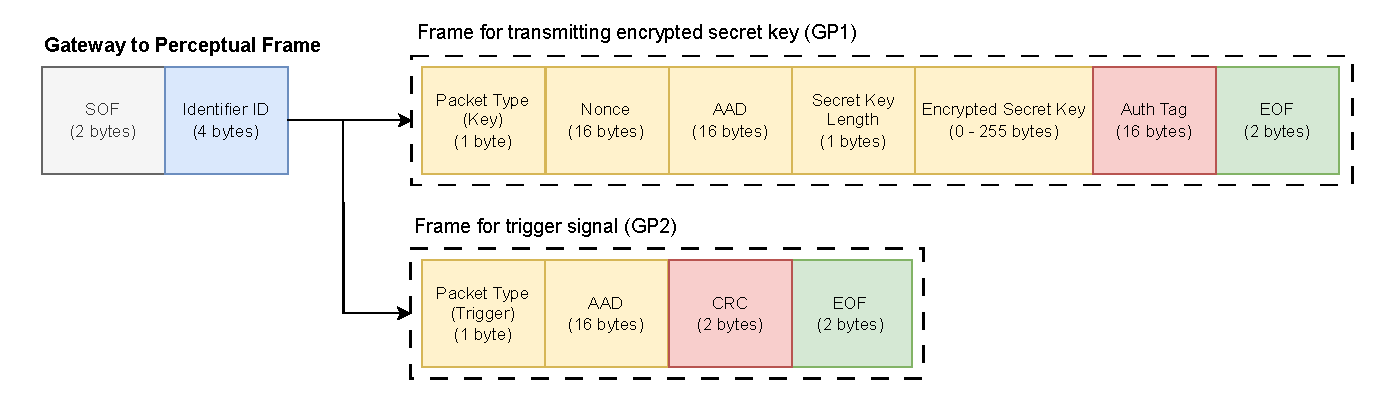
\includegraphics[width=1\linewidth]{gp-frame.pdf}
    \caption{Khung truyền trao truyền dữ liệu từ gateway xuống lớp nhận thức}
    \label{fig:gp}
\end{figure}

Khi nhận tín hiệu kích hoạt (khung GP2) từ gateway, lớp nhận thức sẽ tạo khung PG1 chứa dữ liệu mã hóa và gửi cho gateway (minh họa hình \ref{fig:pg-frame}). Trường dữ liệu của khung PG1 chứa 16-byte \textit{Nonce}, đây là \textit{Nonce} được dùng trong mã hóa dữ liệu và phía máy chủ sẽ dùng \textit{Nonce} này cho giải mã. Tiếp theo, 16-byte Auth Tag sẽ được gửi nhằm xác thực dữ liệu mã hóa, máy chủ sau khi giải mã sẽ so sánh Auth Tag, nếu có sự khác biệt về Auth Tag, máy chủ sẽ từ chối gói tin đó. Ngoài ra, 2-byte \textit{Cyclic Redundancy Check} (CRC) giúp phát hiện có sự sai lệch hay mất mác dữ liệu nào trong quá trình truyền.

\begin{figure}[H]
    \centering
    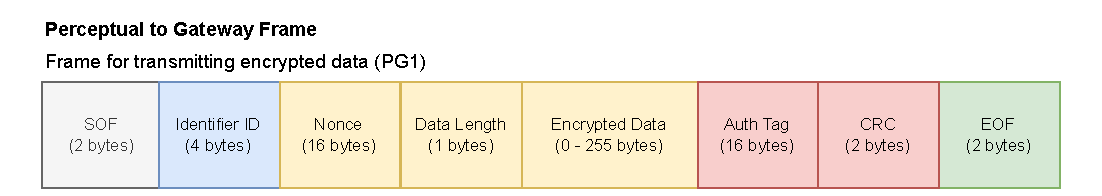
\includegraphics[width=0.9\linewidth]{pg-frame.pdf}
    \caption{Khung truyền trong truyền dữ liệu từ lớp nhận thức lên gateway}
    \label{fig:pg-frame}
\end{figure}

\subsubsection{Khung truyền trong giao tiếp giữa gateway và server}
\label{sec:gs}
Nhóm các khung truyền trong quá trình giao tiếp giữa gateway và máy chủ được minh họa trong Hình \ref{fig:gs-frame}. Tổng cộng có bốn loại khung truyền chính, bao gồm: GS1, GS2, SG1 và một khung truyền đặc biệt dùng để gửi thông tin trạng thái hiện tại của hệ thống lên máy chủ.

Khung truyền GS1 là khung được sử dụng để truyền thông tin về khóa công khai, phục vụ cho quá trình trao đổi khóa giữa gateway và máy chủ. Các trường chuẩn trong cấu trúc khung được giữ nguyên. Trường dữ liệu của khung chứa một \textit{Nonce} có độ dài 16 byte, dùng trong quá trình tính toán thẻ xác thực, tiếp đó là 1-byte \textit{public key length} và phần tải chứa khóa công khai. Do trường dữ liệu chứa thông tin quan trọng, việc bổ sung 16 byte Auth Tag giúp tăng cường bảo mật và hạn chế nguy cơ giả mạo khóa trong quá trình trao đổi. Auth Tag này được tạo ra bằng thuật toán Ascon-128a, sử dụng khóa chia sẻ trước cùng với giá trị $AAD_{key}$ đã được cấu hình sẵn giữa gateway và máy chủ. Để tối ưu hiệu suất tính toán, phần bản rõ (plaintext) được bỏ trống vì chỉ cần tạo Auth Tag. Điều này giúp giảm thời gian xử lý cho cả gateway và máy chủ, đồng thời vẫn đảm bảo tính toàn vẹn của khóa công khai. Sau khi nhận được khung GS1 từ gateway, máy chủ sẽ tiến hành kiểm tra các trường trong khung. Tiếp theo, máy chủ sử dụng thuật toán giải mã Ascon-128a với bản mã (ciphertext) rỗng, cùng với \textit{Nonce} và giá trị $AAD_{key}$ để tính lại Auth Tag. Auth Tag này sau đó được so sánh với Auth Tag nhận được nhằm xác minh tính toàn vẹn của thông tin khóa công khai. Hình \ref{fig:auth_t} minh họa việc tính toán Auth Tag trong quá trình trao đổi khóa.

\begin{figure}[h]
    \centering
    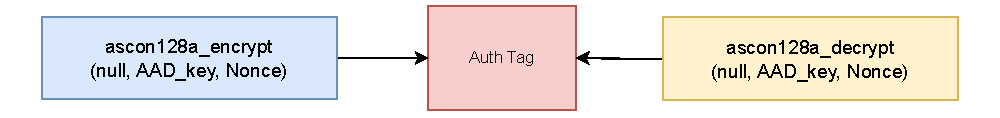
\includegraphics[width=0.85\linewidth]{auth_t.pdf}
    \caption{Tính toán thẻ xác thực (Auth Tag) trong trao đổi khóa}
    \label{fig:auth_t}
\end{figure}

Trong truyền dữ liệu mã hóa từ gateway lên máy chủ, khung truyền GS2 sẽ được sử dụng. Khung truyền này giữ lại các trường tương tự như GS1, tuy nhiên, GS2 được cấu hình thêm một trường 4-byte \textit{sequence number}. Khung truyền GS2 đóng vai trò chính trong quá trình truyền dữ liệu và được sử dụng thường xuyên trong suốt thời gian hệ thống hoạt động. Đây là loại khung được sử dụng phổ biến nhất, do đảm nhiệm chức năng truyền tải dữ liệu giữa gateway và máy chủ một cách liên tục và ổn định. Việc bổ sung 4 byte \textit{sequence number} vào khung truyền giúp tăng cường bảo mật trong quá trình truyền dữ liệu, nhằm ngăn chặn các cuộc tấn công như tấn công phát lại (replay attack) hoặc tấn công xen giữa (Man-in-the-Middle). Khi giải mã khung truyền, máy chủ sẽ kiểm tra sequence number hiện tại của gói tin. Nếu phát hiện bất kỳ sai lệch nào về giá trị này, gói tin sẽ bị từ chối ngay lập tức. Cơ chế này làm giảm nguy cơ tấn công phát lại, vì ngay cả khi kẻ tấn công thu được một gói tin cũ và cố gắng gửi lại, sequence number bên trong gói tin sẽ không còn phù hợp với trạng thái hiện tại, do giá trị này được tăng tuần tự qua từng phiên truyền. Trường dữ liệu của khung GS2 bao gồm một \textit{Nonce} có độ dài 16 byte, một trường \textit{payload length} dài 1 byte, phần tải chứa dữ liệu đã được mã hóa, và cuối cùng là Auth Tag dài 16 byte được tạo ra trong quá trình mã hóa dữ liệu. Các thành phần như Nonce, dữ liệu mã hóa và Auth Tag đều được trích xuất từ khung PG1 do lớp nhận thức gửi lên gateway. Khi máy chủ nhận được khung GS2, nó sẽ tách các trường cần thiết để tái tạo giá trị $AAD_{data}$, phục vụ cho quá trình giải mã và xác thực dữ liệu.

Khung SG1 được sử dụng như một tín hiệu điều khiển gửi từ máy chủ về gateway. Hiện tại, SG1 được cấu hình để phục vụ hai loại tín hiệu chính: tín hiệu xác nhận (ACK) nhằm thông báo rằng phiên truyền dữ liệu đã thành công, và tín hiệu cập nhật sequence number mới. Trong một số tình huống, khi máy chủ xác định cần cập nhật giá trị sequence number, nó sẽ sử dụng khung SG1 để gửi tín hiệu tương ứng đến gateway nhằm đảm bảo sự đồng bộ giữa hai bên.

Cuối cùng là một loại khung truyền đặc biệt, dùng để gửi các thông tin về tình trạng hoạt động của hệ thống, bao gồm các chỉ số như tỷ lệ chuyển gói thành công (PDR – Packet Delivery Ratio), độ trễ, số lượng gói tin đã truyền, và các thông số liên quan khác. Khung truyền này được gửi định kỳ lên máy chủ, thường mỗi vài phút một lần, nhằm cung cấp dữ liệu giám sát giúp người dùng theo dõi và đánh giá hiệu suất của hệ thống.

\begin{figure}
    \centering
    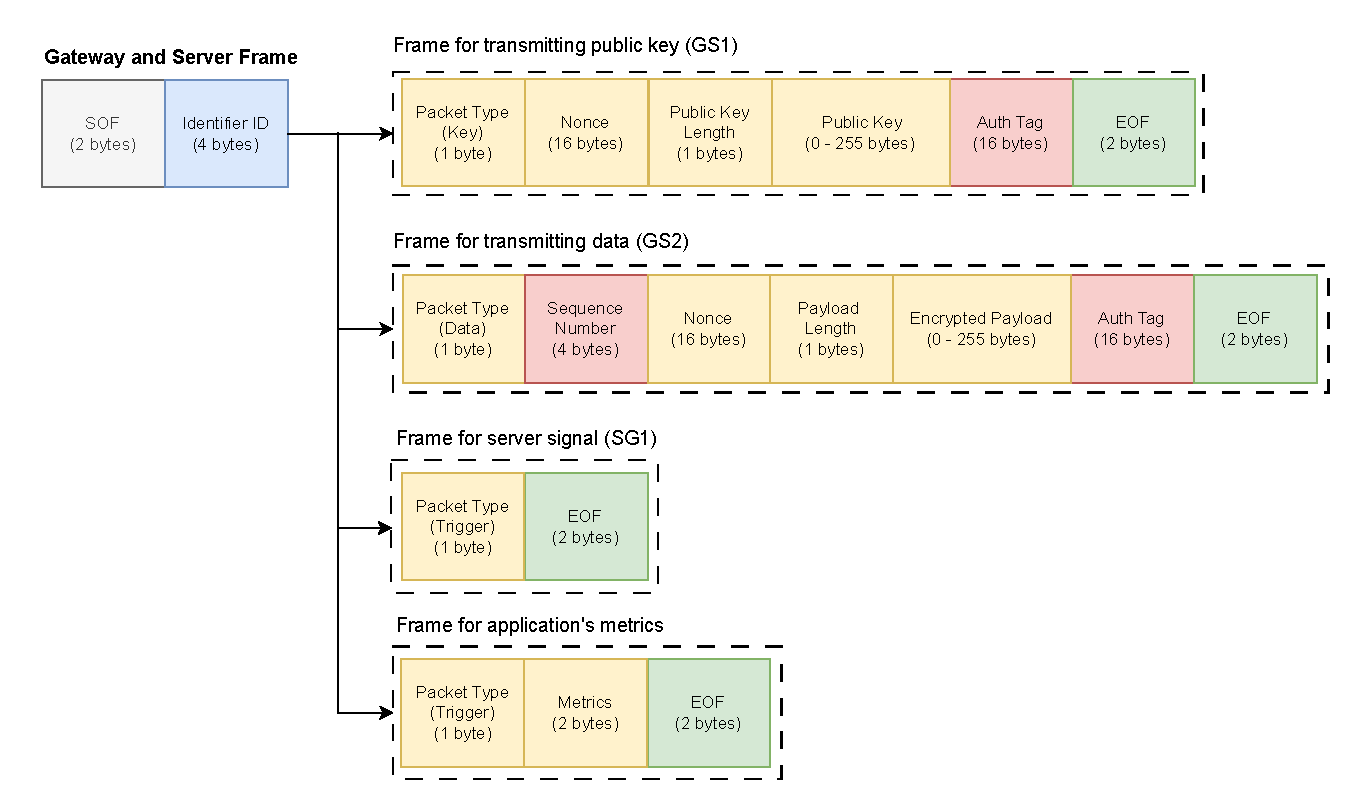
\includegraphics[width=1\linewidth]{gs-frame.pdf}
    \caption{Bộ khung truyền trong giao tiếp giữa gateway và máy chủ}
    \label{fig:gs-frame}
\end{figure}
\subsubsection{Quá trình phân giải khung truyền}
Quá trình phân giải khung truyền được trình bày trong hình \ref{fig:parsing} và \ref{fig:parse-function}. Tất cả các khung truyền được sử dụng trong hệ thống đều áp dụng chung quá trình phân giải này. Vì vậy, để đảm bảo tính ngắn gọn cũng như dễ hiểu trong báo cáo, khung truyền GS2 sẽ được minh họa trong hình để trình bày về quá trình phân giải khung truyền. Việc phân giải bắt đầu từ việc nhận dữ liệu từ thiết bị đích và lưu trữ vào trong một bộ đệm nội bộ (internal buffer), để chuẩn bị cho quá trình phân giải. Mỗi byte trong bộ đệm sẽ được luân phiên đưa vào hàm phân giải khung truyền (Hình \ref{fig:parse-function}). Trong mỗi hàm phân giải, các điều kiện ở mỗi trường trong khung truyền được cấu hình sẵn. Từ đó, hàm phân giải sẽ kiểm tra số byte tương ứng trong bộ đệm nội bộ với điều kiện; nếu điều kiện đúng, hàm phân giải sẽ tiến hành kiểm tra trường tiếp theo; ngược lại, sẽ ngừng quá trình phân giải và trả về mã lỗi. Nếu hàm phân giải có thể phân giải được tất cả các trường trong bộ đệm, quá trình phân giải sẽ hoàn tất. Việc mã hóa dữ liệu sẽ được diễn ra trong quá trình phân giải này, cụ thể là trong bước tính thẻ xác thực. Ở bước này, dữ liệu sẽ được mã hóa, từ đó sinh ra thẻ xác thực, sau đó so sánh với thẻ xác thực nhận được để kiểm tra tính toàn vẹn của dữ liệu. 

\begin{figure}[H]
    \centering
    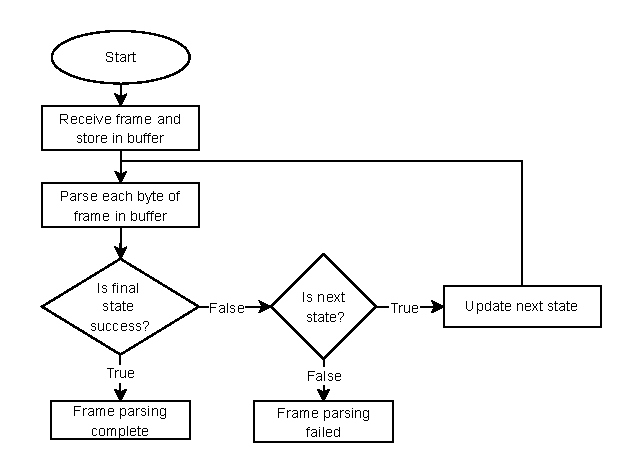
\includegraphics[width=0.7\linewidth]{frameparsing1.pdf}
    \caption{Quá trình phân giải khung truyền}
    \label{fig:parse-function}
\end{figure}

\begin{figure}[H]
    \centering
    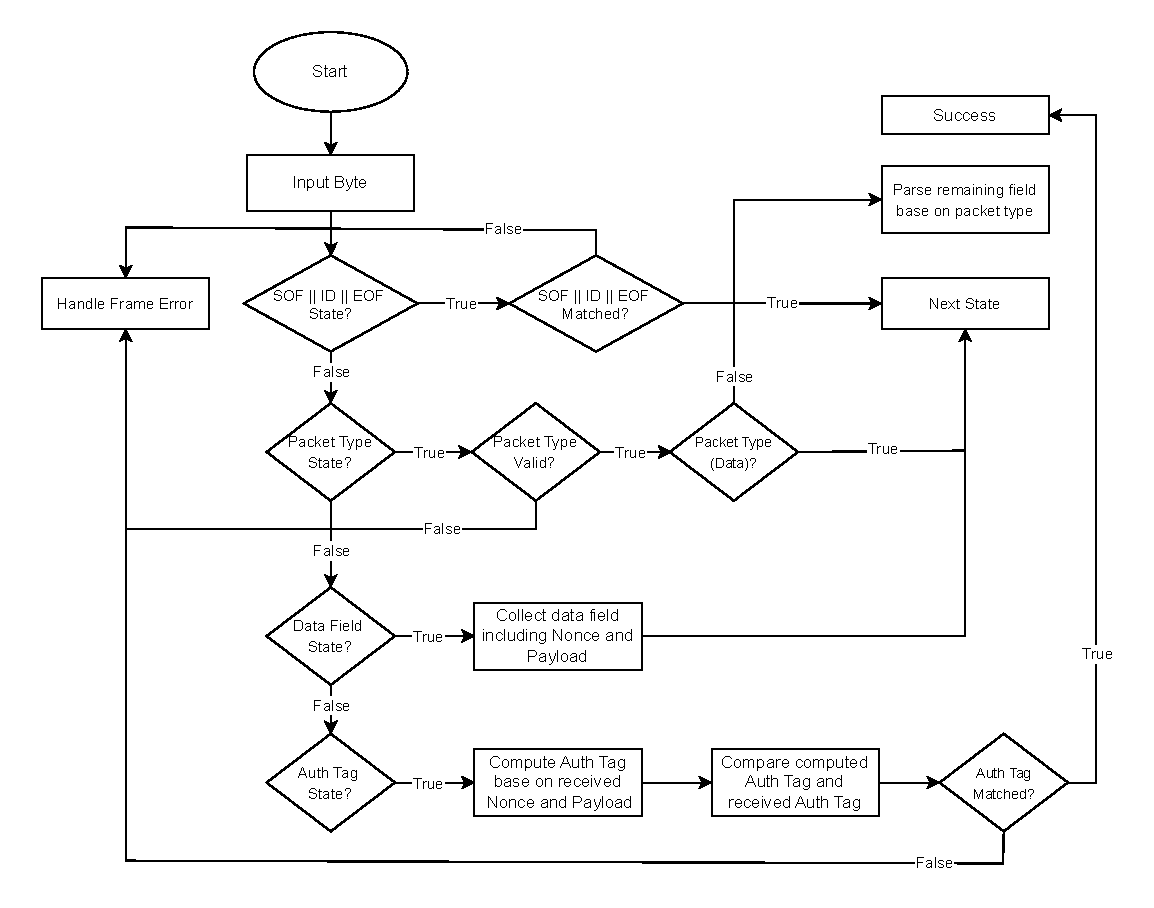
\includegraphics[width=1\linewidth]{frameparse.pdf}
    \caption{Hàm phân giải khung truyền GS2}
    \label{fig:parsing}
\end{figure}

\subsection{Cơ chế safe counter}
\label{sec:safe_counter}
Như đã đề cập ở phần \ref{sec:gs}, khung truyền GS2 được cấu hình thêm 4-byte \textit{sequence number} để hạn chế khả năng tấn công phát lại (replay attack) và tấn công xen giữa (Man-in-the-Middle). Tuy nhiên, một số trường hợp kẻ tấn công có thể gửi rất nhiều gói tin với các \textit{sequence number} khác nhau nhằm cố gắng brute-force thành công \textit{sequence number} hiện tại của hệ thống. Có thể thấy rằng với 4 byte \textit{sequence number}, sau khi toàn bộ không gian $2^{32}$ giá trị được thử, xác suất brute-force thành công sẽ đạt 100\%. Vấn đề đặt ra ở đây là xác suất thành công của brute-force tăng dần theo số lần thử — tức là bài toán mang tính xác suất tích lũy \cite{cumulative}. Để khắc phục điều này, cơ chế \textit{safe counter} được triển khai nhằm chuyển bài toán từ dạng có xác suất tăng dần thành một quá trình với xác suất thành công cố định ở mỗi lần thử, từ đó làm cho brute-force trở nên kém hiệu quả hơn. \textit{Safe counter} thực chất là một biến đếm 32-bit đồng bộ giữa gateway và máy chủ, biến đếm này sẽ được cập nhật liên tục trong quá trình truyền dữ liệu. Trong trường hợp bị brute-force, máy chủ sẽ từ chối các gói tin sai về \textit{sequence number} trong quá trình phân giải, số gói tin mà máy chủ từ chối sẽ được gọi là $R$. Ở máy chủ, một ngưỡng được đặt ra gọi là \(T_{\text{reject}} \), nếu máy chủ từ chối một số lượng gói tin chạm ngưỡng \(T_{\text{reject}} \), hay nói cách khác nếu $R \geq T_{reject}$, máy chủ sẽ ngay lập tức gửi một tín hiệu tới gateway bằng khung truyền SG1 và thực hiện việc cập nhật \textit{sequence number} mới dựa trên \textit{safe counter} hiện tại của hệ thống. Vì \textit{safe counter} được đồng bộ giữa gateway và máy chủ, việc tính toán lại \textit{sequence number} sẽ cho ra kết quả giống nhau, đảm bảo việc truyền dữ liệu giữa gateway và máy chủ vẫn diễn ra bình thường với \textit{sequence number} mới. Thuật toán \ref{alg:safe_counter} trình bày chi tiết cách tính \textit{sequence number} mới dựa trên \textit{safe counter}.
Đối với cách cập nhật \textit{safe counter}, các phép toán dịch bit và \textit{XOR} bit được sử dụng nhằm loại bỏ tính tuyến tính và tăng tính ngẫu nhiên của việc cập nhật. Kết 
quả cuối cùng được \textit{mod} với $2^{32}$ để đảm bảo kết quả luôn nằm trong phạm vi 32 bit. Cách tính này sẽ giúp \textit{safe counter} có tính ngẫu nhiên nhẹ, chống lại
việc đoán giá trị tiếp theo. Để tạo \textit{sequence number} mới, \textit{safe counter} sẽ được kết hợp với khóa bí mật ($K_{master}$) đã được trao đổi trước đó bằng phép toán \textit{XOR},
đảm bảo kẻ tấn công không thể đoán được \textit{sequence number} mới được cập nhật. Sau khi cập nhật thành công, biến đếm $R$ sẽ được reset về 0 để theo dõi lại từ đầu.
\begin{algorithm}[ht]
\caption{Cơ chế safe counter}
\small
\label{alg:safe_counter}
\begin{algorithmic}[1]
\Require 32-bit Safe Counter $SC$, Secret Key $K$, Threshold $T_{\text{rejected}}$, Rejected Packet Count $R$, Current Sequence Number $SN$
\State $SC \gets (SC + ((SC \ll 3) \oplus (SC \gg 2) \oplus 7)) \bmod 2^{32}$
\If{$R \geq T_{\text{rejected}}$}
    \State $SN \gets (SC \oplus K) \bmod 2^{32}$
    \State $R \gets 0$
\EndIf
\Return $SN$
\end{algorithmic}
\end{algorithm}

Với cơ chế này, kẻ tấn công sẽ có \(T_{\text{reject}} \) cơ hội để đoán trước khi \textit{sequence number} được cập nhật lại một giá trị mới ngẫu nhiên. Tỉ lệ đoán thành công \textit{sequence number} sau \(T_{\text{reject}} \) lần thử có công thức là:
\[
P_{\text{guess}} \approx 1 - \left(1 - \frac{1}{2^{32}}\right)^{T_{\text{rejected}}}.
\]
Trong hệ thống thử nghiệm, \(T_{\text{reject}} \) được đặt mặc định là 10, vì thế tỉ lệ cố định để có thể brute-force thành công \textit{sequence number} là:
\[
P_{\text{guess}} \approx 1 - \left(1 - \frac{1}{2^{32}}\right)^{10} \approx 0.00000023 \%
\]
Thử nghiệm trên 70,000 gói tin giả mạo với các \textit{sequence number} khác nhau được gửi vào hệ thống, kết quả cho thấy máy chủ từ chối hoàn toàn 70,000 gói tin, đạt tỉ lệ chính xác 100\%, cho thấy được độ tin cậy cao của cơ chế này. 

% Hình \ref{fig:sclog} trình bày quá trình cập nhật và đồng bộ \textit{sequence number} mới giữa gateway và máy chủ thông qua \textit{safe counter}:

% \begin{figure}[ht]
%     \centering
%     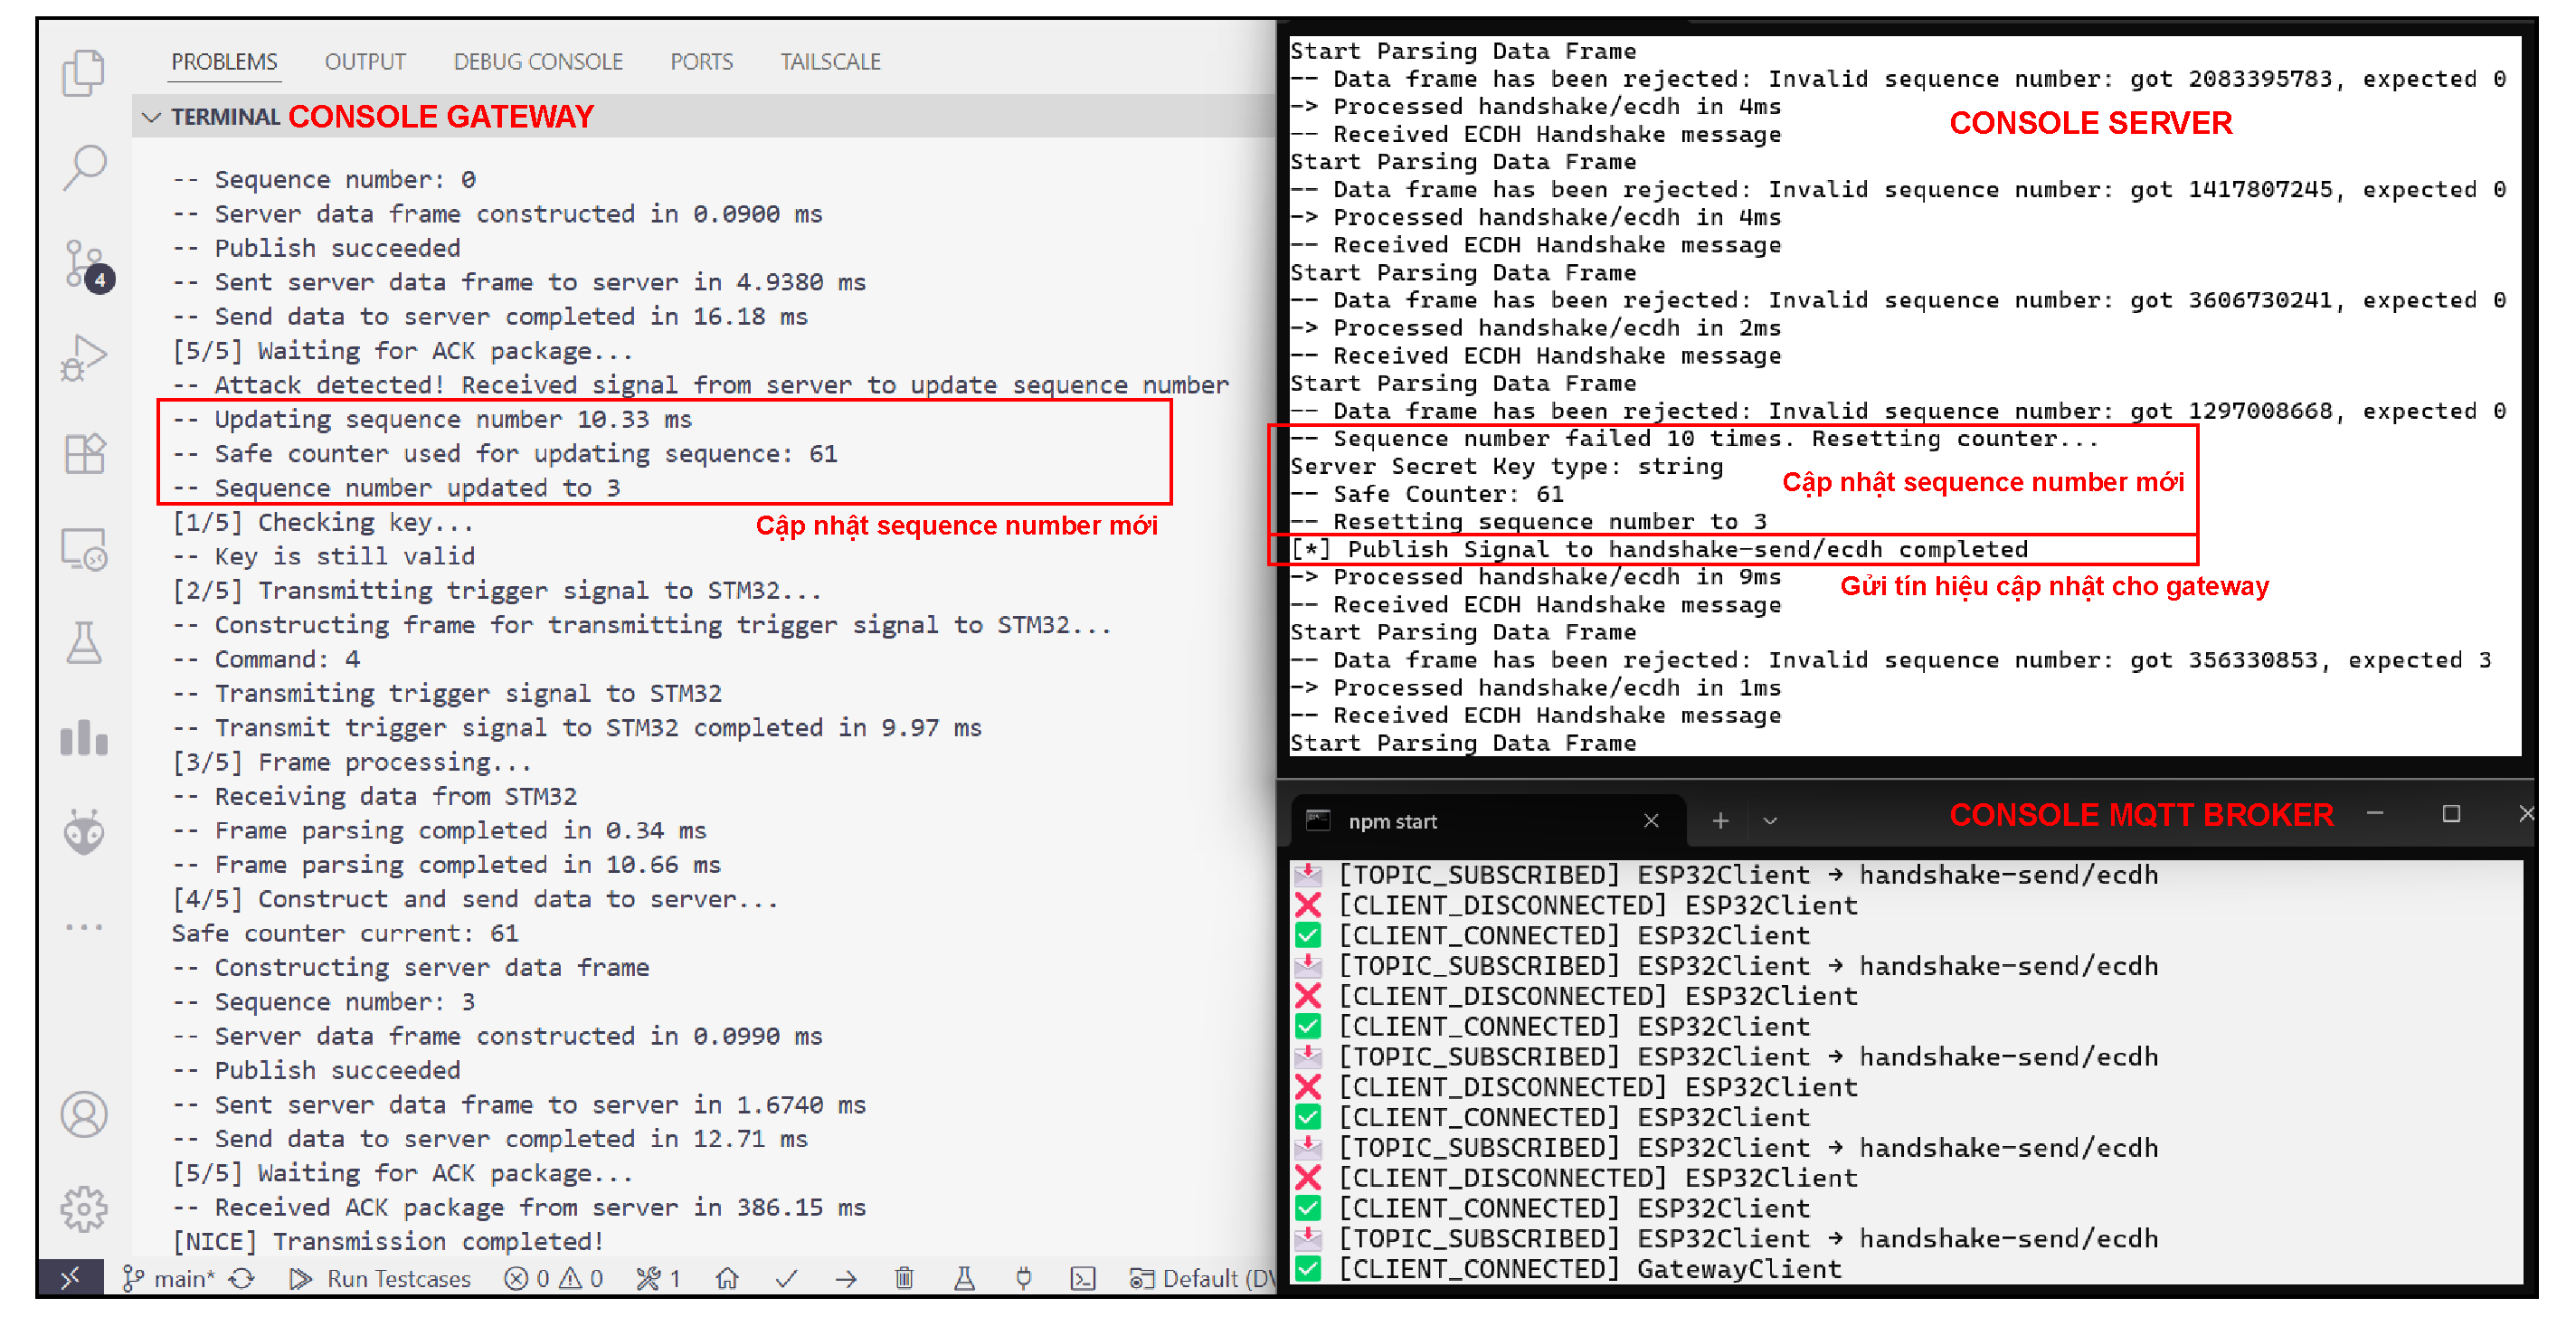
\includegraphics[width=1\linewidth]{sclog.pdf}
%     \caption{Log của gateway và máy chủ trong quá trình cập nhập}
%     \label{fig:sclog}
% \end{figure}

% \subsection{Triển khai máy chủ}
% Máy chủ đóng vai trò trung tâm trong hệ thống IoT, chịu trách nhiệm tiếp nhận dữ liệu từ gateway, xử lý và phân giải các gói tin, kiểm tra tính hợp lệ của gói tin, sau đó cung cấp thông tin đến người dùng cuối. Đối với các gói tin không hợp lệ, máy chủ có khả năng từ chối ngay lập tức để không ảnh hưởng đến người dùng. Trong kiến trúc hệ thống này, máy chủ được cấu hình để thực hiện một số chức năng quan trọng liên quan đến bảo mật và xử lý dữ liệu. Thuật toán trao đổi khóa ECDH được sử dụng để thiết lập khóa chung giữa gateway, trong khi thuật toán Ascon-128a đảm nhiệm việc giải mã và xác thực dữ liệu nhận được. Ngoài ra, máy chủ còn sử dụng hàm băm Ascon Hash nhằm tạo ra khóa phiên cho quá trình giải mã. Hệ thống máy chủ được triển khai trên nền tảng Node.js, với JavaScript là ngôn ngữ lập trình chính, giúp đảm bảo khả năng mở rộng, xử lý bất đồng bộ hiệu quả và dễ dàng tích hợp với các thành phần khác trong hệ thống. Hình \ref{fig:sg} trình bày mô hình giao tiếp giữa gateway và máy chủ sử dụng giao thức MQTT.

% \begin{figure}[H]
%     \centering
%     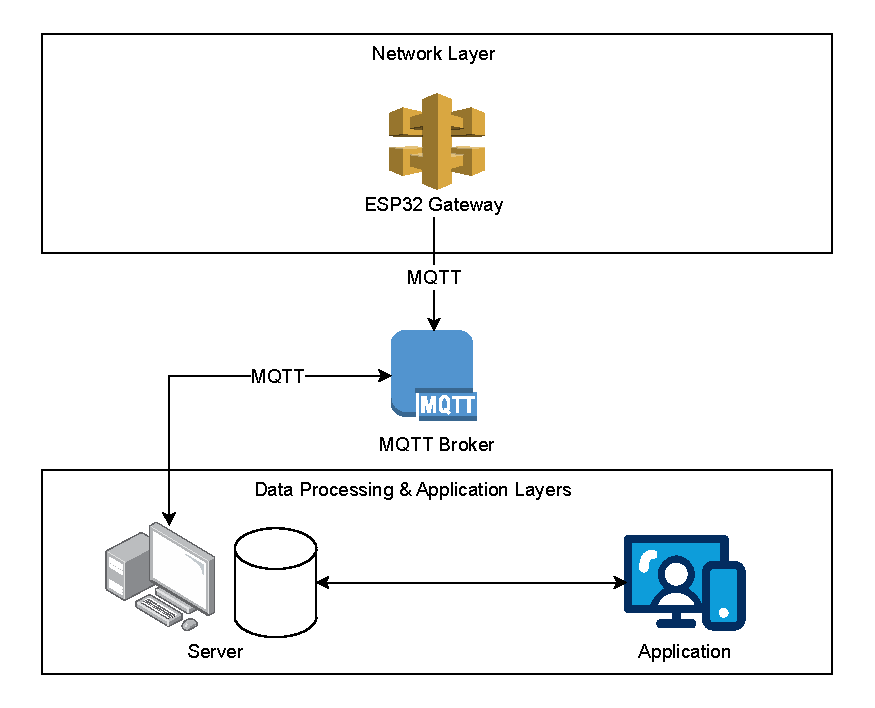
\includegraphics[width=0.75\linewidth]{servergateway.pdf}
%     \caption{MQTT trong giao tiếp giữa gateway và máy chủ}
%     \label{fig:sg}
% \end{figure}

\chapter{Kết quả triển khai và phân tích}
\label{Chapter4}

\section{Mô hình thực nghiệm}
Hệ thống IoT được xây dựng dựa trên kiến trúc IoT bốn lớp được đề xuất. Ở lớp nhận thức, vi điều khiển STM32F411VET6 được sử dụng, hoạt động với tần số 16 MHz. Ở lớp mạng, sử dụng module ESP32 với tần số 240 MHz, đóng vai trò là gateway, tổng hợp và luân chuyển dữ liệu lên máy chủ với cấu hình của máy chủ được trình bày trong bảng \ref{tab:server-config}. Đối với quá trình trao đổi khóa giữa máy chủ và gateway, mô hình được cấu hình sẵn thời gian giữa các lần trao đổi khóa là một phút, nhằm dễ đánh giá việc chi phí tính toán của thuật toán ECDH ảnh hưởng đến hệ thống như thế nào. Tuy nhiên, thời gian trao đổi khóa có thể được cấu hình khác nhau trong thực tế, tùy vào khả năng tính toán của hệ thống, năng lượng tiêu thụ và yêu cầu về bảo mật. Thời gian giữa mỗi lần truyền dữ liệu được đặt là 1 ms.

\begin{table}[ht]
\centering
\small
\caption{Cấu hình máy chủ}
\label{tab:server-config}
\renewcommand{\arraystretch}{1.2} % Increase vertical spacing
\begin{tabular}{|p{3cm}|p{10cm}|}
\hline
\textbf{Thành phần} & \textbf{Cấu hình} \\
\hline
OS      & Ubuntu 18.04.6 LTS \\
RAM     & 7.8 GiB \\
Storage & 97 GiB \\
CPU     & Intel(R) Xeon(R) CPU E5504 2.00 GHz \\
\hline
\end{tabular}
\end{table}

\section{Kết quả, phân tích và đánh giá}
Phần này nêu ra các kết quả thực hiện và hiệu suất của hệ thống. Đồng thời, đánh giá một số ưu nhược điểm của hệ thống cũng như khả năng chống lại một số cuộc tấn công phổ biến.
\subsection{Kết quả thực hiện}
Trên MCU STM32F411VET6, các kỹ thuật bao gồm kiến trúc khung truyền, kỹ thuật tạo khóa phiên và mã hóa dữ liệu sử dụng thuật toán mã hóa nhẹ Ascon-128a đã được triển khai thành công. Hình \ref{fig:stm32log} trình bày kết quả thực hiện mã hóa và tạo khóa phiên bằng Debugger trên công cụ CubeIDE. Đối với mỗi quá trình tạo khóa và mã hóa thành công, các biến kiểm tra sẽ được đặt thành 1 để báo quá trình thành công. Giá trị \textit{session\_key\_index} thể hiện thứ tự phiên hiện tại trong quá trình giao tiếp, là tham số được sử dụng trong hàm tạo khóa phiên.
\begin{figure}[h]
    \centering
    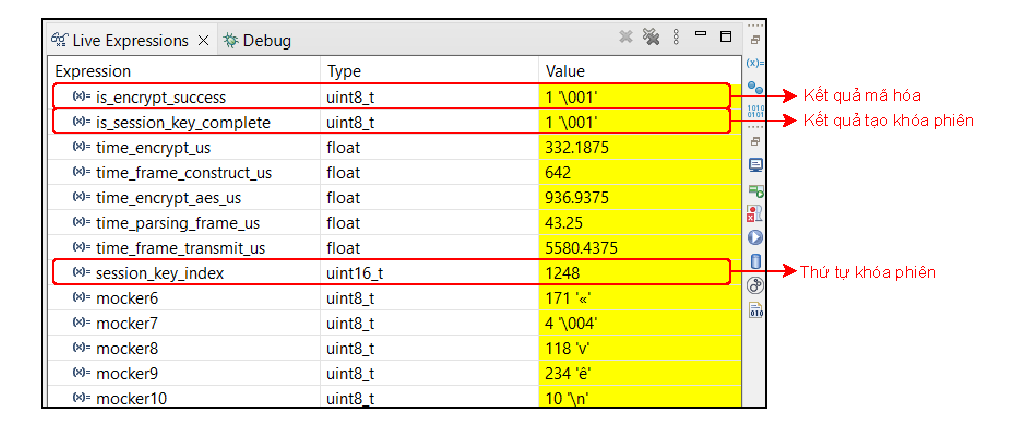
\includegraphics[width=0.8\linewidth]{stm32log.pdf}
    \caption{Kết quả thực hiện trên MCU STM32F411VET6}
    \label{fig:stm32log}
\end{figure}

Khi hệ thống được reboot, quá trình khởi tạo ngay lập tức hoạt động. ESP32 gửi một tín hiệu yêu cầu gói tin khởi tạo từ máy chủ. Sau đó, máy chủ sẽ xác minh thiết bị yêu cầu và gửi về dữ liệu khởi tạo. Dữ liệu khởi tạo này sau đó sẽ được ESP32 tiếp tục chuyển tiếp xuống STM32 ở lớp nhận thức. Kết quả thực hiện quá trình này được trình bày trong hình \ref{fig:initlog}.

\begin{figure}[h]
    \centering
    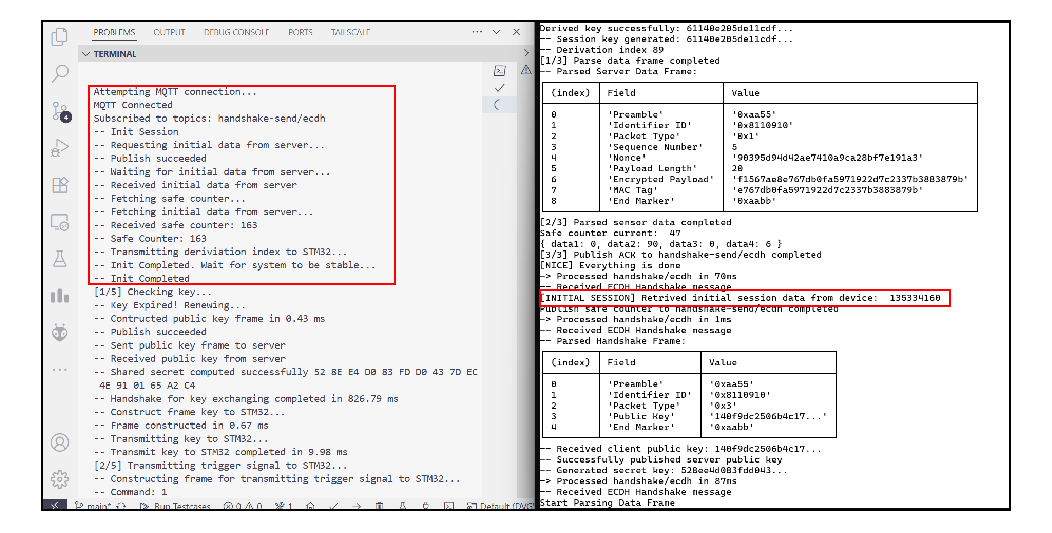
\includegraphics[width=1\linewidth]{initlog.pdf}
    \caption{Quá trình khởi tạo khi reboot}
    \label{fig:initlog}
\end{figure}

Kỹ thuật trao đổi khóa sử dụng thuật toán ECDH được triển khai thành công trên ESP32 IoT Gateway và hệ thống Backend. Thứ tự thực hiện quá trình trao đổi khóa được thực hiện chính xác bao gồm gửi khóa chung, nhận khóa chung và tính toán khóa bí mật. Các khóa chung khi publish đều được cấu trúc bằng khung truyền. Hình \ref{fig:logecdh} trình bày kết quả thực hiện trên ESP32 Gateway và máy chủ.

\begin{figure}[h]
    \centering
    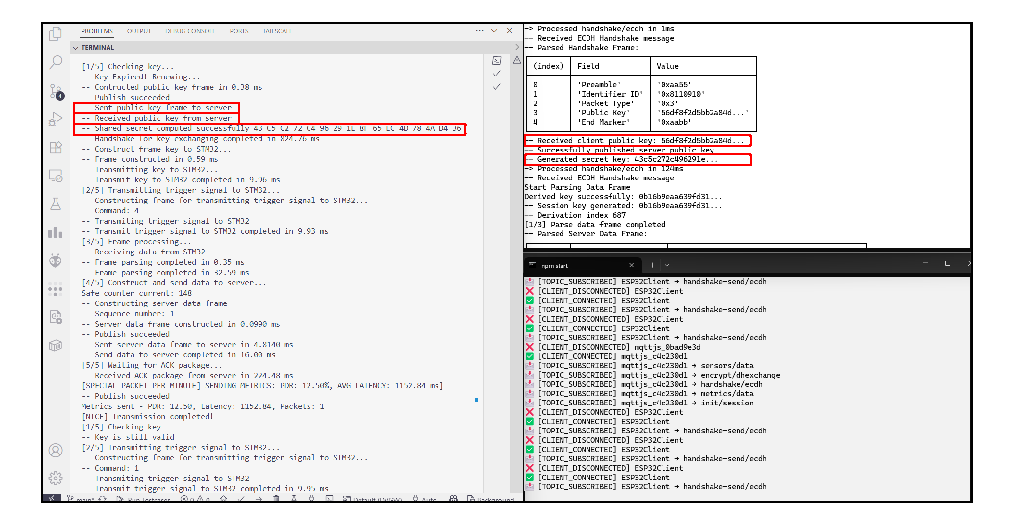
\includegraphics[width=1\linewidth]{ecdhlog.pdf}
    \caption{Quá trình trao đổi khóa giữa gateway và máy chủ}
    \label{fig:logecdh}
\end{figure}

Quá trình truyền dữ liệu được triển khai thành công theo đúng trình tự được trình bày trong hình \ref{fig:system} và \ref{fig:trans-sys}. Trên ESP32, quá trình truyền được chia thành năm giai đoạn chính bắt đầu bằng việc kiểm tra khóa, gửi tín hiệu kích hoạt đến cho STM32 ở lớp nhận thức, nhận khung dữ liệu từ STM32 và tiến hành phân giải, tạo khung truyền dữ liệu mới đề gửi lên máy chủ, cuối cùng chờ tín hiệu ACK từ máy chủ. Về phần máy chủ, sau khi nhận khung truyền đã phân giải và mã hóa dữ liệu thành công sẽ gửi về tín hiệu ACK để kết thúc phiên. Các kết quả giao tiếp trên được trình bày trong hình \ref{fig:datalog}.
\begin{figure}[h]
    \centering
    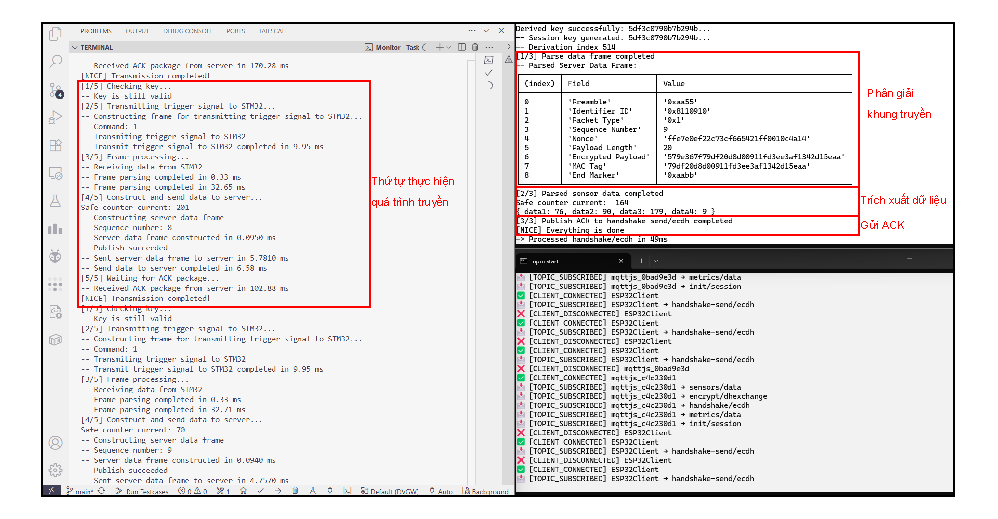
\includegraphics[width=1\linewidth]{datalog.pdf}
    \caption{Quá trình truyền dữ liệu}
    \label{fig:datalog}
\end{figure}

Cơ chế \textit{Safe counter} cũng được triển khai thành công trên cả ESP32 IoT Gateway và máy chủ. Khi phát hiện có dấu hiệu của brute-force thông qua việc máy chủ từ chối quá nhiều gói tin trong khoảng thời gian ngắn, máy chủ sẽ gửi một yêu cầu tạo lại \textit{sequence number} mới thông qua\textit{safe counter}. Hình \ref{fig:sclog} trình bày quá trình cập nhật và đồng bộ \textit{sequence number} mới giữa gateway và máy chủ.

\begin{figure}[h]
    \centering
    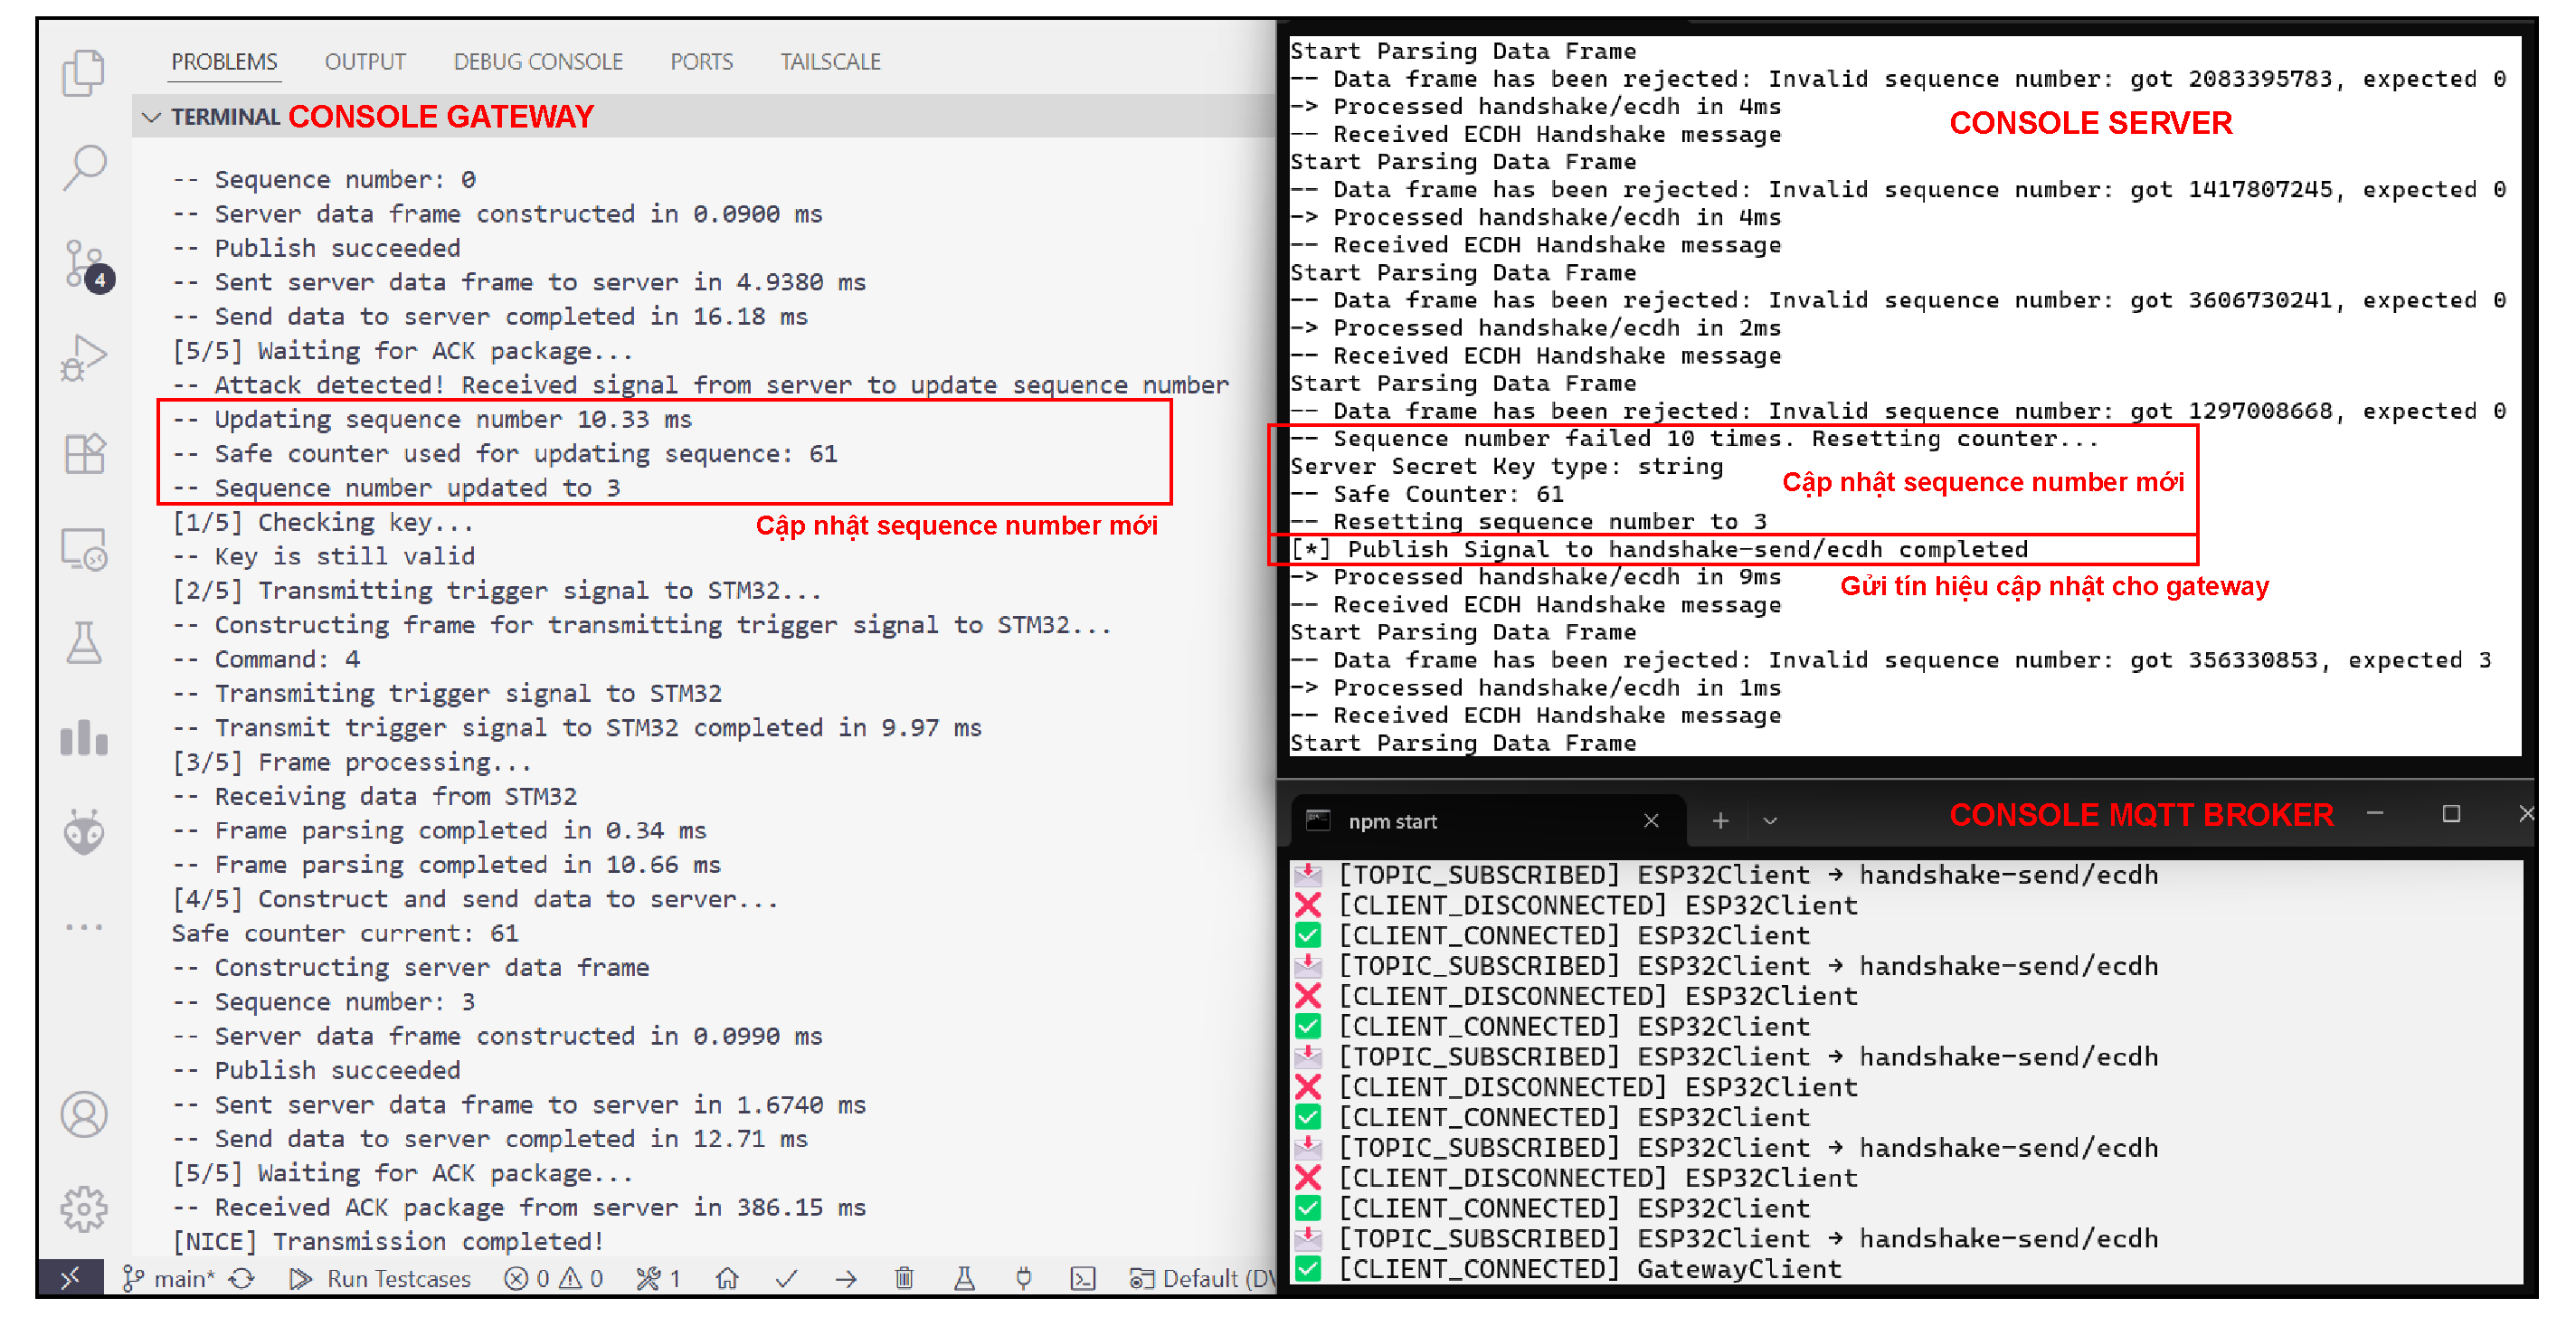
\includegraphics[width=1\linewidth]{sclog.pdf}
    \caption{Quá trình thực hiện cơ chế \textit{safe counter}}
    \label{fig:sclog}
\end{figure}

\subsection{Đánh giá}
\label{sec:res}
Hệ thống được đánh giá dựa trên quá trình trao đổi dữ liệu liên tục trong 120 phút, với các kết quả được trình bày trong hình \ref{fig:stm32}, \ref{fig:esp32} và hình \ref{fig:ke}. Kết quả này tập trung vào hiệu suất của hai thiết bị công suất thấp ở lớp nhận thức và lớp mạng. Đầu tiên là đánh giá với STM32F411VET6 ở lớp nhận thức. STM32 thực hiện việc cấu hình khung truyền PG1 với thời gian trung bình là 0.634 ms. Truyền khung PG1 bằng UART lên gateway có thời gian trung bình là 5.58 ms. Thuật toán Ascon-128a có thời gian mã hóa trung bình là 0.328 ms, cho thấy hiệu năng vượt trội so với thuật toán AES, vốn được triển khai tương tự bằng thư viện X-CUBE-CRYPTOLIB và có thời gian mã hóa trung bình là 0.936 ms trên lõi ARM Cortex-M4. Quá trình phân giải khung truyền GP1 từ gateway có thời gian trung bình là 0.374 ms; khung truyền GP2 có thời gian trung bình là 0.023 ms. Sự khác biệt lớn về thời gian trong quá trình phân giải phần lớn là do việc giải mã khóa và tính toán thẻ xác thực ở khung truyền GP1.

Ở lớp mạng, ESP32 thực hiện việc phân giải PG1 từ STM32 trong thời gian trung bình 0.35 ms. Cấu hình khung truyền GP1 có thời gian trung bình là 0.57 ms, trong khi đó thời gian cấu hình GP2 có thời gian trung bình là 0.014 ms. Thời gian truyền khung truyền GP2 dùng UART xuống lớp nhận thức có thời gian trung bình là 9.01 ms. Quá trình trao đổi khóa bao gồm việc tạo cặp khóa cá nhân (private key)/khóa công khai (public key) và tính toán khóa bí mật có thời gian trung bình lần lượt là 335.08 ms và 335.46 ms. Tuy nhiên, việc trao đổi khóa chỉ được thực hiện sau một khoảng thời gian cố định, vì vậy nếu xét về tổng thể sẽ không ảnh hưởng nhiều đến toàn bộ hiệu suất của hệ thống. Thời gian trung bình cấu hình khung truyền GS1 và GS2 lần lượt là 0.28 ms và 0.033 ms. Mặc dù GS2 có nhiều trường cần cấu hình hơn GS1, nhưng GS2 chỉ thực hiện việc tách trường dữ liệu và thẻ xác thực từ khung PG1 mà không thực hiện tính toán nào thêm. Vì thế, việc cấu hình GS2 nhanh hơn nhiều so với GS1, khi mà GS1 cần phải tính toán thẻ xác thực trong quá trình cấu hình. Thời gian tính toán khóa phiên ở mỗi phiên truyền dữ liệu có thời gian trung bình là 1.189 ms.

Lệnh ACK phản hồi từ máy chủ, báo hiệu phiên truyền thành công, có độ trễ trung bình là 29.58 ms, tính từ lúc khung truyền GS tới máy chủ và gateway nhận được ACK. Tuy nhiên, độ trễ này là không cố định do phụ thuộc phần lớn vào tốc độ mạng cũng như hiệu suất của máy chủ; vì vậy, nếu triển khai ở một số hệ thống khác thì độ trễ sẽ có thể khác. Tổng thời gian truyền được tính từ lúc STM32 nhận được tín hiệu kích hoạt từ gateway cho đến khi gateway nhận được ACK là 51.09 ms.

\begin{figure}[H]
    \centering
    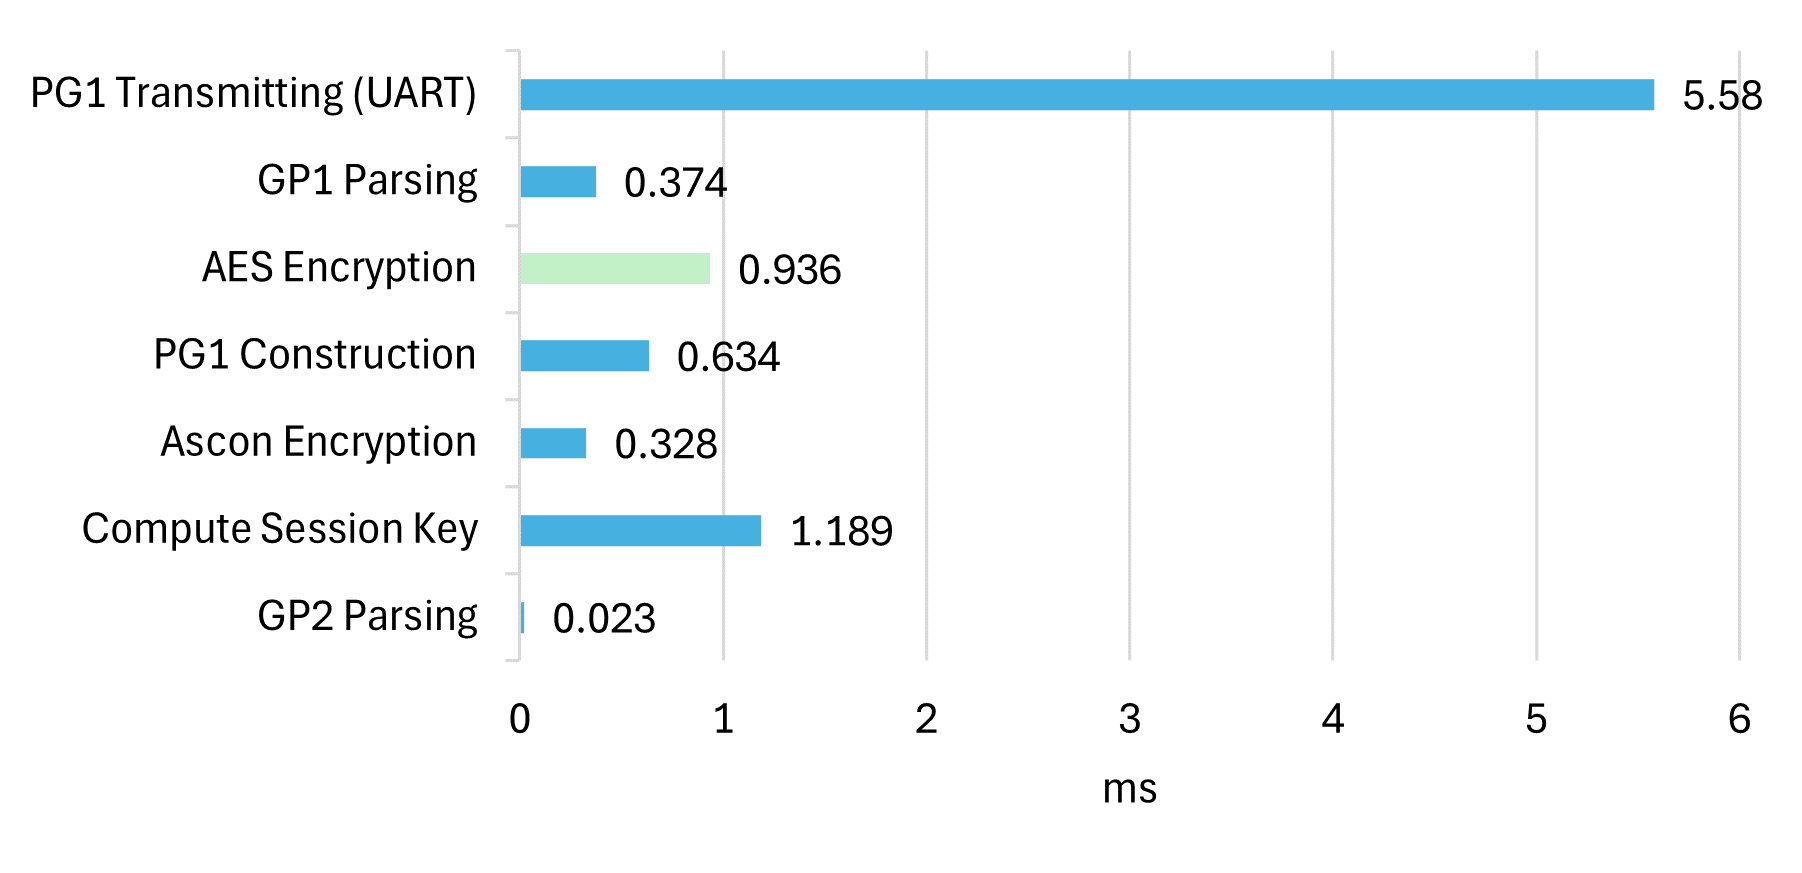
\includegraphics[width=0.75\linewidth]{stm32-2.png}
    \caption{Đánh giá hiệu suất thực thi của STM32F411VET6}
    \label{fig:stm32}
\end{figure}

\begin{figure}[H]
    \centering
    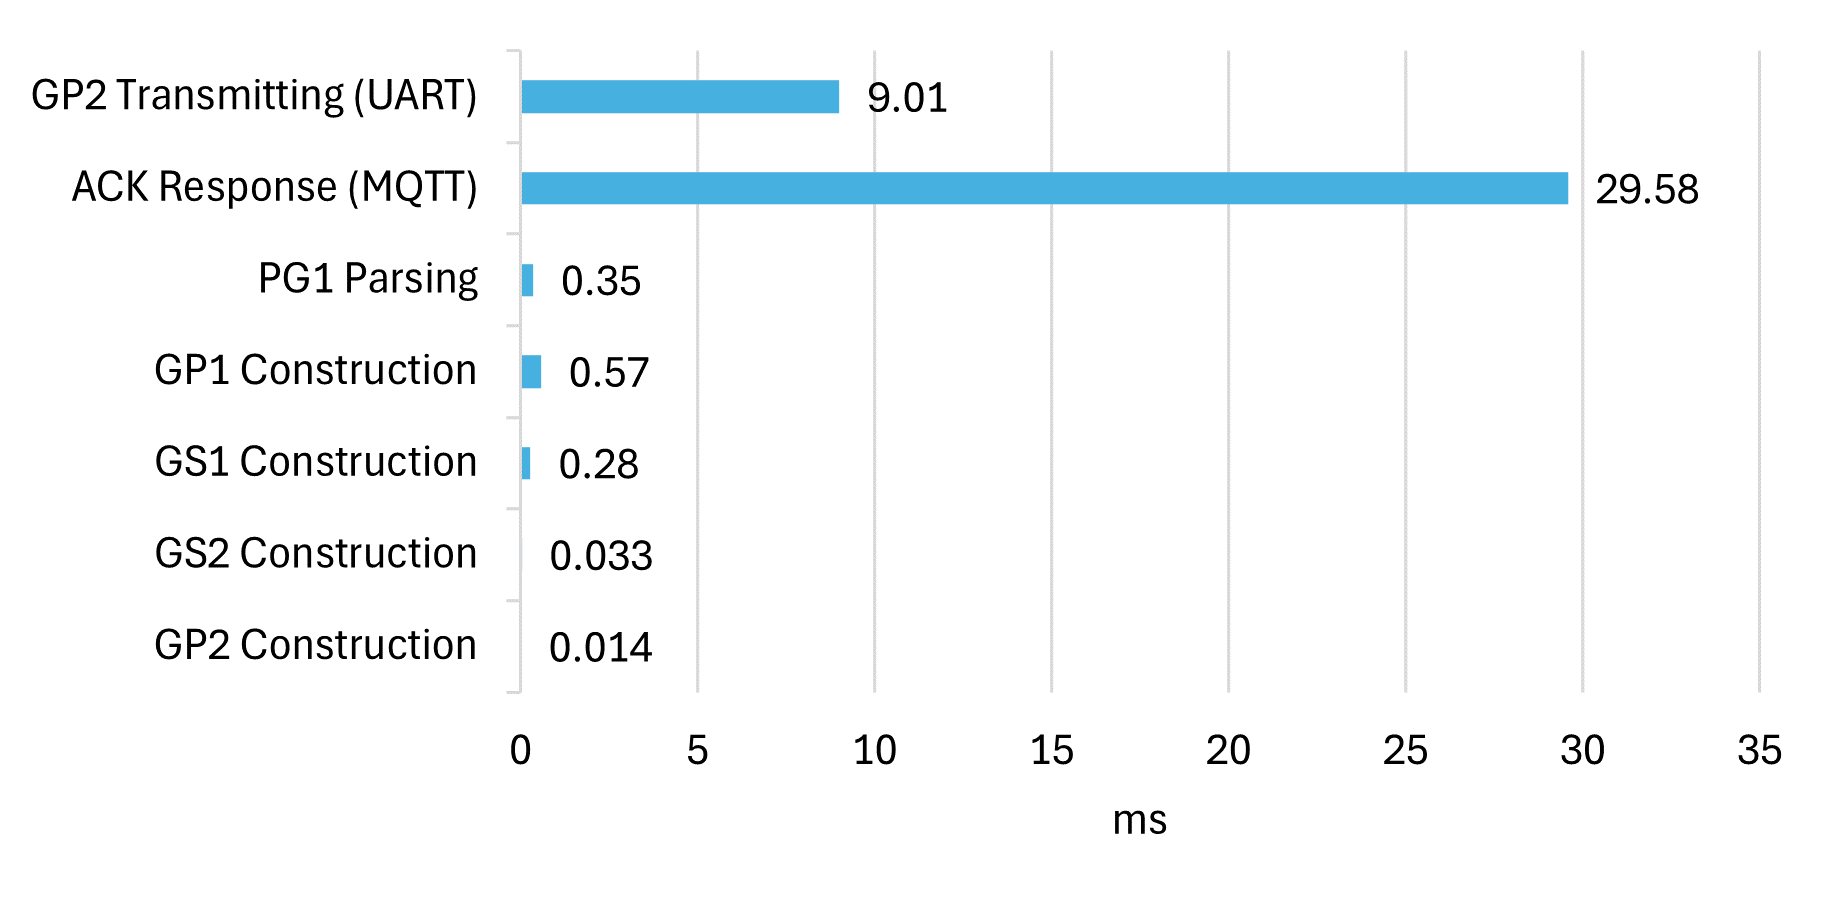
\includegraphics[width=0.75\linewidth]{esp32.png}
    \caption{Đánh giá hiệu suất thực thi của ESP32}
    \label{fig:esp32}
\end{figure}

\begin{figure}[H]
    \centering
    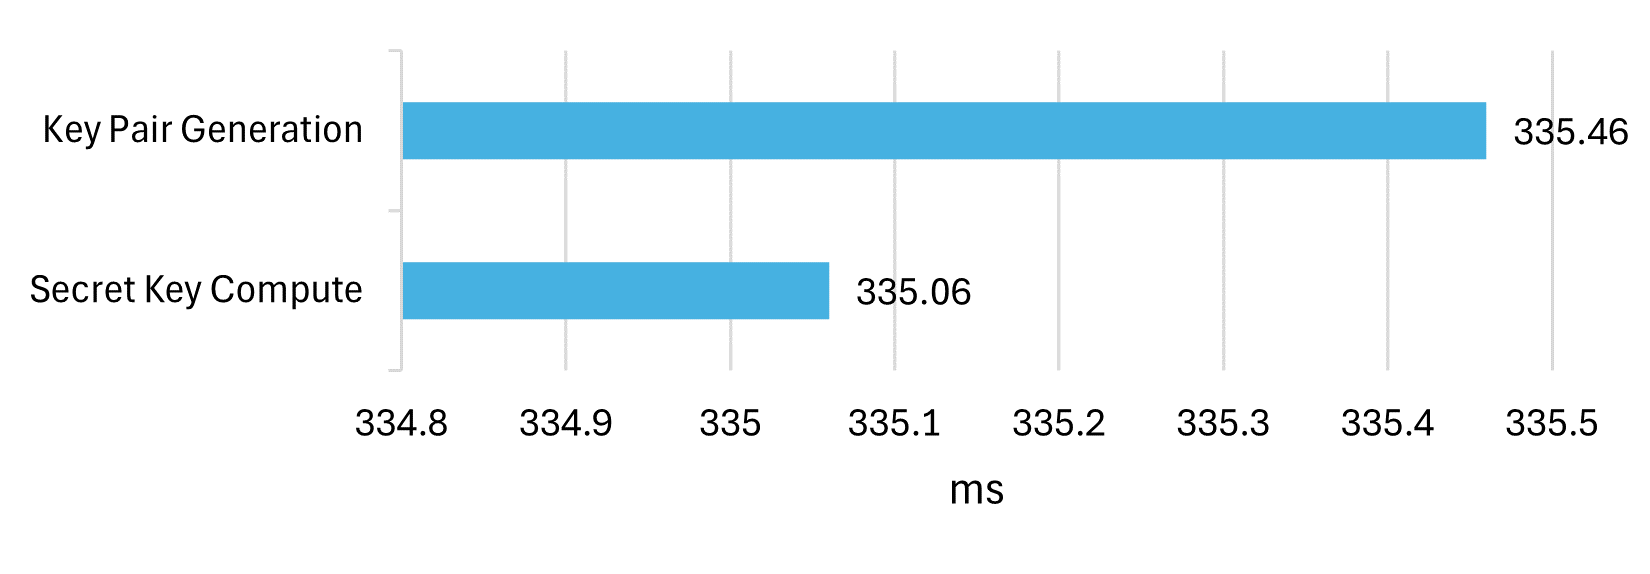
\includegraphics[width=0.75\linewidth]{ke.png}
    \caption{Thời gian thực thi quá trình trao đổi khóa trên ESP32}
    \label{fig:ke}
\end{figure}

Trong khoảng thời gian 120 phút thực nghiệm, gateway đã thực hiện truyền tổng cộng 147,682 gói tin. Một gói tin truyền thành công được định nghĩa là gói tin được mã hóa đúng cách và máy chủ có thể giải mã đúng gói tin đó. Tỷ lệ truyền gói tin thành công (Packet Delivery Ratio - PDR) là một thông số quan trọng trong việc đánh giá mức độ toàn vẹn của hệ thống được tính toán sau mỗi phút truyền dữ liệu, được tính toán với công thức sau:
\[
\text{PDR} = \frac{N_{\text{successful}}}{N_{\text{total}}} \times 100\% 
\]

\begin{align*}
\text{Trong đó:} \quad & N_{\text{successful}} \text{ là số gói tin được nhận thành công tại đích (gói/phút),} \\
                       & N_{\text{total}} \text{ là tổng số gói tin được gửi từ nguồn (gói/phút).}
\end{align*}

Biểu đồ trong Hình \ref{fig:packet} minh họa số lượng gói tin được truyền trong mỗi phút trong suốt 120 phút hoạt động liên tục, với số lượng trung bình đạt 1231 gói/phút. Biểu đồ trong hình \ref{fig:pdr} cho thấy tỷ lệ truyền gói tin mỗi phút cũng trong tổng thời gian 120 phút. Kết quả cho thấy tỷ lệ 100\% được duy trì trong phần lớn thời gian truyền, trong các khoảng thời gian còn lại, tỷ lệ được duy trì ổn định trong khoảng từ 99.8\% cho đến 99.975\%. Tỷ lệ truyền gói tin trung bình là 99.99\%, cho thấy mức độ ổn định và toàn vẹn của hệ thống trong suốt quá trình thực nghiệm. Bảng \ref{tab:performance_metrics} tóm tắt các chỉ số hiệu năng, bao gồm tỷ lệ truyền thành công trung bình, số gói tin trên mỗi khoảng thời gian, và thời gian truyền cho mỗi gói tin.

\begin{figure}[H]
    \centering
    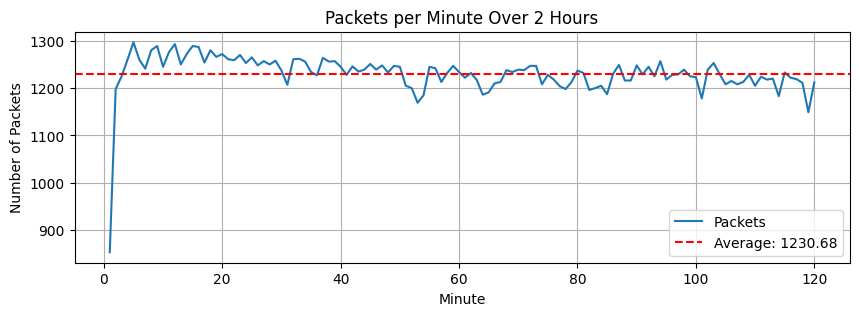
\includegraphics[width=0.8\linewidth]{packet2.png}
    \caption{Số lượng gói tin truyền mỗi phút}
    \label{fig:packet}
\end{figure}

\begin{figure}[H]
    \centering
    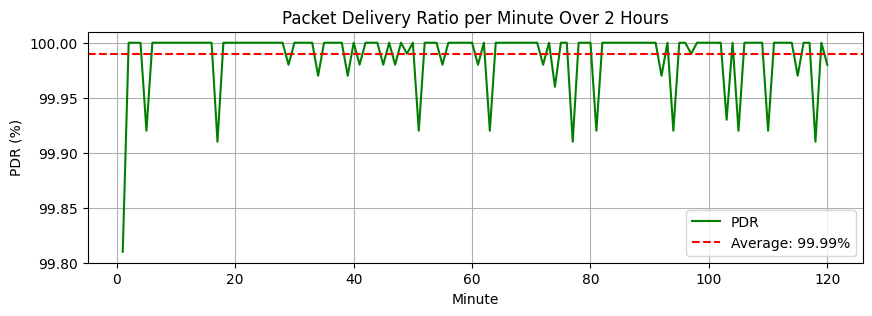
\includegraphics[width=0.8\linewidth]{pdr2.png}
    \caption{Tỷ lệ truyền gói tin mỗi phút}
    \label{fig:pdr}
\end{figure}

\begin{table}[H]
    \centering
    \small
    \caption{Bảng đánh giá hiệu năng trong 120 phút}
    \label{tab:performance_metrics}
    \begin{tabular}{|p{10cm}|p{4cm}|}
        \hline
        \textbf{Thông số} & \textbf{Giá trị} \\
        \hline
        Tổng số gói tin truyền & 147,682 gói tin \\
        Thời gian truyền trung bình & 51.09 ms \\
        Số gói tin truyền trung bình mỗi phút & 1231 gói tin \\
        Tỷ lệ truyền thành công (PDR) & 99.99\% \\
        \hline
    \end{tabular}
\end{table}

Dung lượng bộ nhớ của hệ thống IoT trên ESP32 và STM32 được cung cấp bởi công cụ lập trình PlatformIO và Cube IDE, hiển thị tổng số byte RAM và FLASH được sử dụng trong quá trình nạp firmware. Chi tiết được trình bày trong bảng \ref{tab:memory}.

\begin{table}[h]
\centering
\small
\caption{Dung lượng bộ nhớ RAM và FLASH}
\label{tab:memory}
\begin{tabular}{|p{4cm}|p{5cm}|p{3cm}|}
\hline
Thiết bị & RAM (kB) & Flash (kB) \\
\hline
STM32F411VET6   & 2.34  & 38.22  \\
ESP32-WROOM-32  & 51.04 & 1008.01 \\
\hline
\end{tabular}
\end{table}

Trên STM32F411VET6, nhiệm vụ chính là thu thập và mã hóa dữ liệu, với bộ nhớ chủ yếu dành cho thuật toán Ascon-128a, nhưng tổng thể chiếm dụng không đáng kể. Ngược lại, gateway ESP32 thực hiện nhiều chức năng hệ thống như cấu hình khung truyền và quản lý mạng, thực hiện quá trình trao đổi và quản lý khóa, dẫn đến dung lượng FLASH chiếm nhiều do yêu cầu lập trình đa tác vụ. Hình~\ref{fig:stm32mem} và~\ref{fig:esp32mem} trình bày mức sử dụng bộ nhớ trên hai nền tảng. Cụ thể, trên STM32, bộ nhớ FLASH còn trống 473.78 kB (92.53\%) và RAM còn trống 125.66 kB (98.17\%), cho thấy dung lượng sử dụng là rất thấp. Trong khi đó, trên ESP32, bộ nhớ FLASH chỉ còn trống 291.99 kB (22.46\%) và RAM còn trống 276.96 kB (84.43\%). Như vậy, có thể thấy kiến trúc hệ thống này chủ yếu yêu cầu bộ nhớ FLASH lớn trên gateway ESP32, do cần tích hợp nhiều chức năng hệ thống, trong khi thiết bị cảm biến STM32 hoạt động nhẹ, chủ yếu tập trung vào việc mã hóa dữ liệu với mức tiêu thụ bộ nhớ tối thiểu.

\begin{figure}[H]
\centering
\begin{subfigure}[b]{0.45\textwidth} 
         \centering
         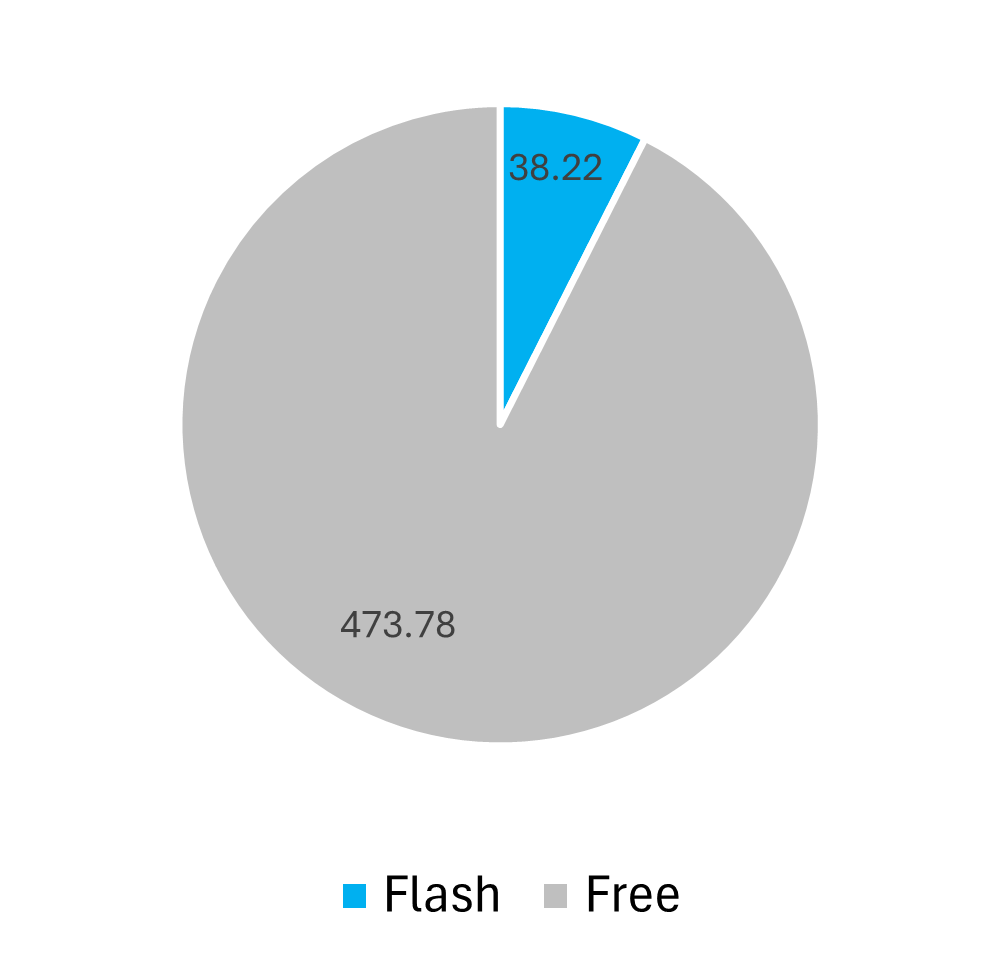
\includegraphics[width=\textwidth]{images/stm32flash.png}
         \caption{Dung lượng Flash}
\end{subfigure}
\hfill
\begin{subfigure}[b]{0.45\textwidth}
         \centering
         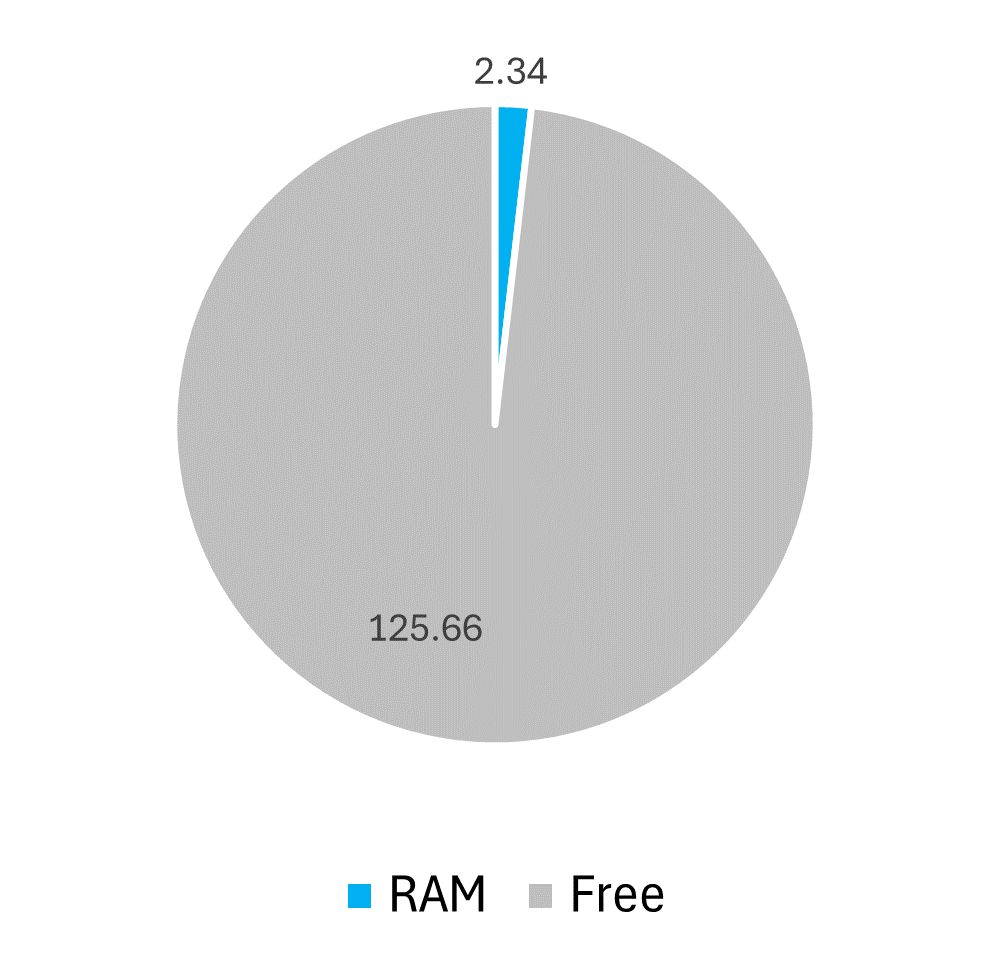
\includegraphics[width=\textwidth]{images/stm32ram.png}
         \caption{Dung lượng RAM}
\end{subfigure}
\caption{Dung lượng tiêu thụ của STM32F411VET6}
\label{fig:stm32mem}
\end{figure}

\begin{figure}[H]
\centering
\begin{subfigure}[b]{0.45\textwidth} 
         \centering
         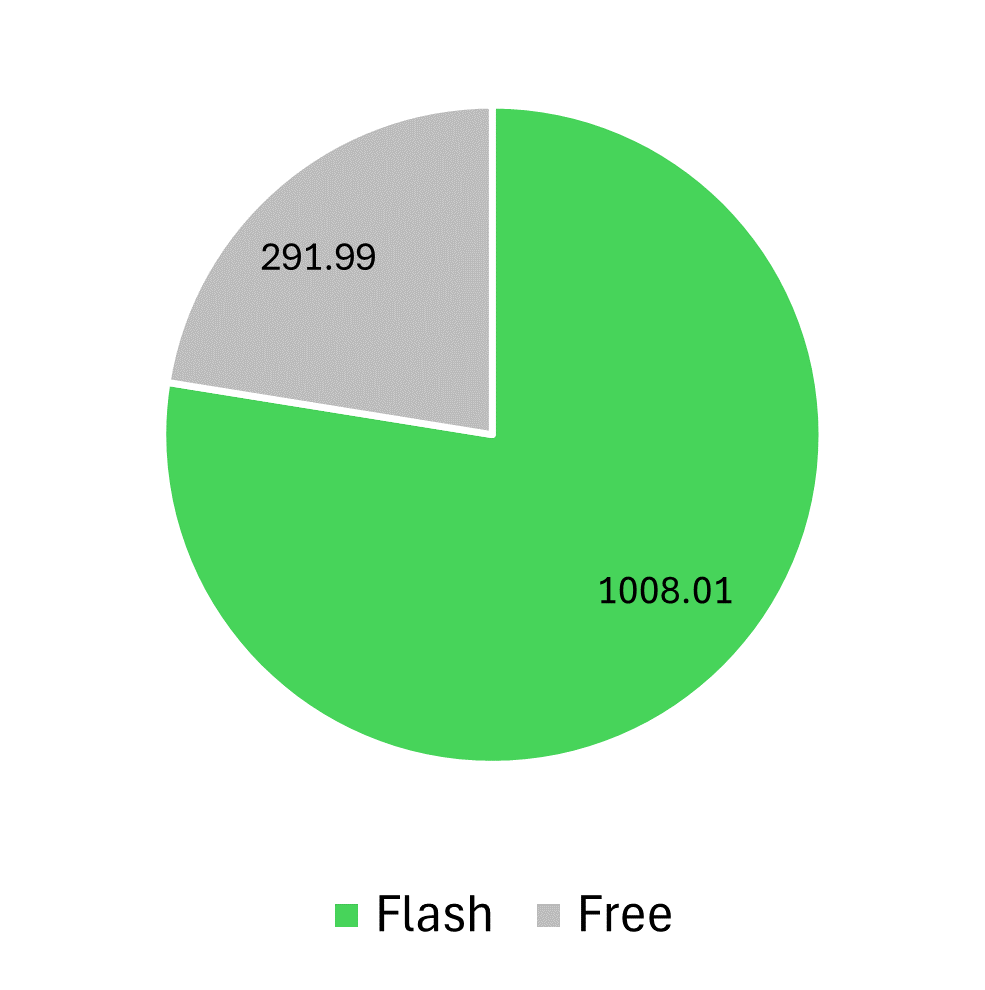
\includegraphics[width=\textwidth]{images/esp32flash.png}
         \caption{Dung lượng Flash}
\end{subfigure}
\hfill
\begin{subfigure}[b]{0.45\textwidth}
         \centering
         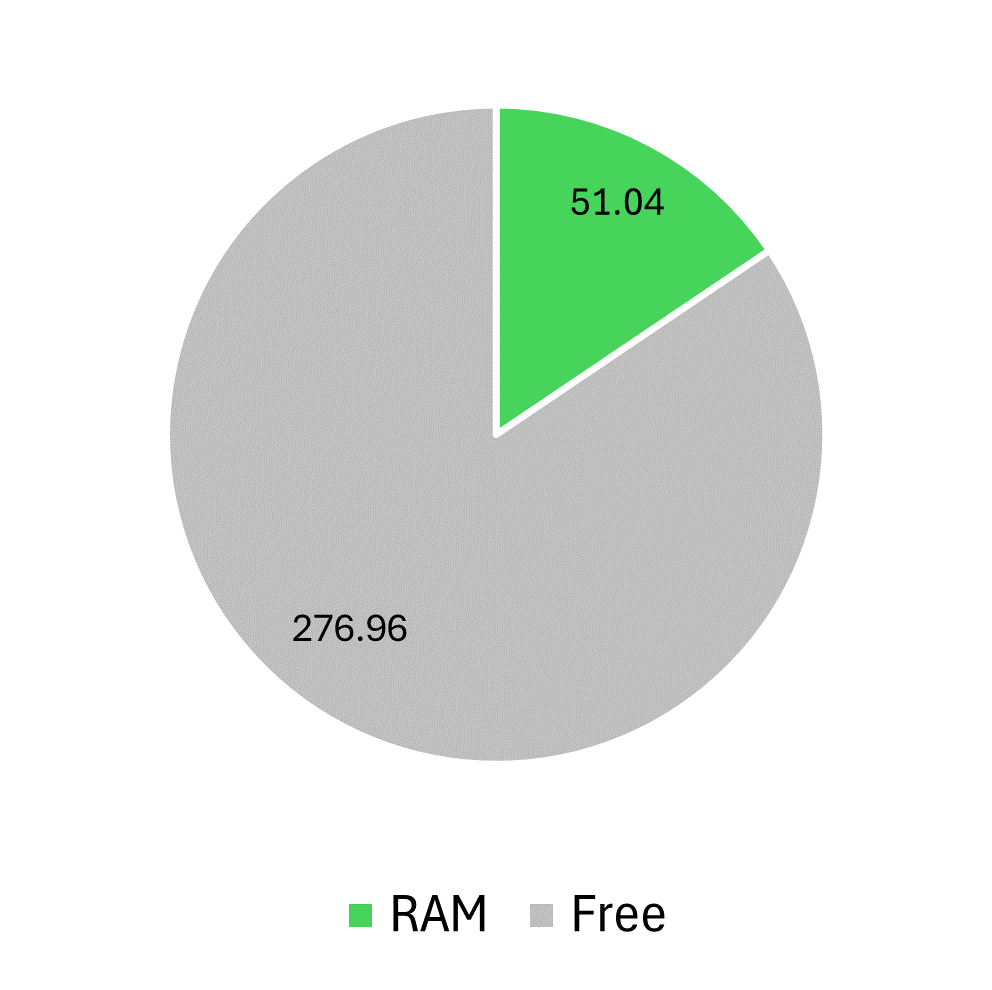
\includegraphics[width=\textwidth]{images/esp32ram.png}
         \caption{Dung lượng RAM}
\end{subfigure}
\caption{Dung lượng tiêu thụ của ESP32-WROOM-32}
\label{fig:esp32mem}
\end{figure}

\subsection{Phân tích thông lượng và hiệu suất tải dữ liệu}
Thông lượng và hiệu suất tải dữ liệu là hai thông số quan trọng trong việc đánh giá hệ thống. Việc sử dụng kiến trúc khung truyền với các trường dữ liệu bổ sung sẽ tốn thêm chi phí truyền tải, kích thước mỗi gói tin sẽ tăng so với các phương pháp đơn giản hơn. Phần này sẽ tập trung vào phân tích thông lượng và hiệu suất tải dữ liệu để đánh giá một số hạn chế của hệ thống. Đồng thời, đề xuất một số phương pháp có thể giúp cải thiện hệ thống trong tương lai.

Khung truyền GS2 sẽ được sử dụng trong việc đánh giá thông lượng cũng như hiệu suất tải dữ liệu của hệ thống. Đây là khung truyền được sử dụng với tần suất lớn nhất trong suốt quá trình truyền tải dữ liệu. Khung truyền GS2 là khung truyền đảm nhận việc truyền dữ liệu từ lớp nhận thức đến máy chủ bằng giao thức MQTT. Thông qua việc phân tích khung truyền GS2, có thể xấp xỉ chính xác nhất thông lượng và hiệu suất tải dữ liệu của hệ thống. Tổng kích thước của khung truyền GS2 là tổng kích thước của tất cả các trường dữ liệu được tính toán như sau:
\begin{align*}
\text{Size}_{GS2} &= \text{SOF (2)} + \text{ID (4)} + \text{Packet Type (1)} + \text{Seq. Number (4)} \\
& \quad + \text{Nonce (16)} + \text{Payload Length (1)} + \text{Encrypted Payload (3)} \\
& \quad + \text{Auth Tag (16)} + \text{EOF (2)} \\
&= 49\ \text{bytes}
\end{align*}
Trong hệ thống đã triển khai, lớp nhận thức thu thập và truyền tải 3 byte dữ liệu, từ đó tham số \textit{Encrypted Payload} cũng có kích thước là 3 byte. Một điều chú ý đó là tổng kích thước của khung truyền GS2 sẽ có sự thay đổi dựa trên kích thước dữ liệu mà lớp nhận thức muốn truyền tải. Từ kết quả đó được ở phần \ref{sec:res}, trong 120 phút, hệ thống đã truyền tải tổng cộng 147,682 gói tin. Tuy nhiên, vì phần này chỉ đánh giá thông lượng của khung truyền GS2, 120 khung truyền GS1 trong việc trao đổi khóa sẽ bị loại bỏ trong tính toán. Dẫn đến tổng số gói tin sử dụng khung truyền GS2 sẽ được tính là:
\[
\text{Total}_{GS2} = 147,682 - 120 = 147,562 \ \text{(gói tin)}
\]
Tổng kích thước mà hệ thống đã truyền tải sẽ được tính như sau:
\[
\text{Total}_{size} = 147,562 \times 49 = 7,230,538 \ \text{(byte)}
\]
Từ đó, ta có thể tính toán thông lượng của hệ thống bằng công thức:
\[
\textit{Throughtput} = \left( \frac{\text{Data size}}{\text{Transmission Time}} \right) \times 8 = \left( \frac{7,230,538}{120 \times 60} \right) \times 8 \approx 8,033.93 \ \text{bps}
\]
Trong đánh giá này, mỗi khung truyền GS2 có tổng kích thước là 49 byte, tuy nhiên chỉ có 3 byte dữ liệu cần thiết, phần còn lại chủ yếu là các trường bổ sung nhằm đảm bảo tính bảo mật của hệ thống, dẫn đến một tham số được đưa ra đó là hiệu suất tải (\textit{payload efficiency}) khá nhỏ là $3/49 \approx 6.12\%$. Con số này nói lên rằng chỉ có 6.12\% dữ liệu được truyền là dữ liệu hữu ích, trong khi phần còn lại là chi phí truyền dẫn khác không có ý nghĩa đối với người dùng cuối. Vì vậy, mặc dù thông lượng của hệ thống khá cao nhưng thực tế thì thông lượng hữu ích (goodput) lại thấp hơn nhiều:
\[
\textit{Goodput} = \left( \frac{147,562 \times 3}{120 \times 60} \right) \times 8 \approx 491.87 \ \text{bps}
\]
Từ những phân tích trên, có thế thấy chi phí truyền tải khi áp dụng kiến trúc khung truyền là không nhỏ. Với hiệu suất tải thấp sẽ dẫn đến việc tiêu tốn băng thông, băng thông sẽ không được sử dụng một cách tối ưu. Tuy nhiên, hiệu suất tải sẽ được cải thiện đáng kể nếu hệ thống truyền nhiều dữ liệu, tức là kích thước tải lớn hơn. Bảng \ref{tab:efficiency} trình bày hiệu suất tải với các kích thước tải khác nhau trên cũng một khung truyền dữ liệu, có thể thấy thay vì truyền 3 byte dữ liệu như đề tài đã thực hiện, nếu ứng dụng kiến trúc này vào các hệ thống cần truyền nhiều dữ liệu đồng thời, việc sử dụng băng thông sẽ được tối ưu hơn rất nhiều.
\begin{table}[h]
\centering
\small
\caption{Hiệu suất tải với các kích thước tải khác nhau}
\label{tab:efficiency}
\begin{tabular}{|p{4cm}|p{5cm}|p{3cm}|}
\hline
Payload Length & Total Frame Size & Efficiency \\
\hline
3 bytes   & 49 bytes  & 6.12\%  \\
10 bytes  & 56 bytes & 17.85\% \\
20 bytes  & 66 bytes & 30.30\% \\
50 bytes  & 96 bytes & 52.08\% \\
\hline
\end{tabular}
\end{table}
\subsection{Phân tích khả năng bảo mật của hệ thống}
Phần này trình bày đánh giá chi tiết về mức độ an toàn của hệ thống IoT được đề xuất, thông qua việc phân tích và nhận xét khả năng kháng cự của nó trước một số dạng tấn công phổ biến hiện nay.

\textit{Nhận xét 1: Hệ thống có khả năng chống lại các cuộc tấn công từ bên ngoài như Man-in-the-Middle}
\begin{itemize}
    \item Trong kiến trúc đề xuất, tất cả các lớp trong mô hình IoT bốn lớp đều được mã hóa bằng thuật toán mã hóa xác thực Ascon-128a. Nhờ đó, dù kẻ tấn công có xâm nhập và đánh cắp dữ liệu tại bất kỳ lớp nào trong quá trình truyền giữa, dữ liệu vẫn không thể bị giải mã hay sử dụng trái phép. Cơ chế này giúp đảm bảo tính bảo mật và toàn vẹn của thông tin người dùng trong toàn bộ hệ thống.
\end{itemize}

\textit{Nhận xét 2: Cơ chế khung truyền được thiết kế để ngăn chặn các thiết bị không hợp lệ giao tiếp với hệ thống.}
\begin{itemize}
    \item Với thiết kế khung truyền dữ liệu, đảm bảo rằng chỉ có những thiết bị cùng một hệ sinh thái mới có thể giao tiếp và truyền dữ liệu cho nhau. Các thiết bị khác ở bên ngoài sẽ không có khả năng gửi dữ liệu vì không khớp ở các trường như SOF, Identifier ID và EOF, đây vốn là những trường độc nhất được cấu hình riêng cho mỗi thiết bị.
\end{itemize}

\textit{Nhận xét 3: Cơ chế khung truyền đảm bảo tính toàn vẹn của dữ liệu.}
\begin{itemize}
    \item Trước khi truyền, dữ liệu luôn được cấu trúc lại thành khung truyền bao gồm các trường xác thực. Khi một lớp trong hệ thống tiếp nhận khung truyền, dữ liệu sẽ được kiểm tra thông qua hàm phân giải nhằm xác thực tính hợp lệ. Cơ chế này giúp phát hiện và loại bỏ các sai sót trong quá trình truyền, đảm bảo rằng dữ liệu đến đích luôn chính xác. Điều này được thể hiện thông qua chỉ số PDR đạt 99.99\% trong quá trình thử nghiệm.
\end{itemize}

\textit{Nhận xét 4: Quá trình trao đổi khóa được đảm bảo an toàn nhờ tích hợp thẻ xác thực (Auth Tag) trong khung truyền.}
\begin{itemize}
    \item Để bảo vệ quá trình trao đổi khóa, khóa công khai được truyền với khung truyền được tích hợp 16 byte Auth Tag. Với sự kết hợp của Auth Tag, đảm bảo rằng kể cả khi có kẻ tấn công từ bên ngoài muốn gửi khóa công khai giả nhằm phá hoại việc tính toán khóa bí mật, hệ thống vẫn có thể phát hiện và từ chối các khóa giả ngay lập tức. 
\end{itemize}

\textit{Nhận xét 5: Thuật toán trao đổi khóa ECDH đảm bảo mức độ bảo mật theo khuyến nghị của NIST.}
\begin{itemize}
    \item Quá trình trao đổi khóa dùng thuật toán ECDH sử dụng đường cong \textit{sect163k1} với mức bảo mật là 80-bit. Mức bảo mật này đáp ứng được khuyến nghị của NIST về mức độ bảo mật \cite{nist}. Hơn nữa, khóa bảo mật sẽ được cập nhật định kỳ, khiến các cuộc tấn brute-force vào khóa bí mật trở nên không khả thi.
\end{itemize}

\textit{Nhận xét 6: Hệ thống có khả năng phát hiện và ngăn chặn các cuộc tấn công phát lại (replay attack).}
\begin{itemize}
    \item Với 4 byte \textit{sequence number} được tích hợp trong khung truyền GS2, đảm bảo rằng máy chủ có thể phát hiện và từ chối bất kỳ gói tin nào bị gửi lại do không trùng khớp \textit{sequence number}. Nhờ đó, các cuộc tấn công phát lại sẽ không thể làm gián đoạn hệ thống.
\end{itemize}

\textit{Nhận xét 7: Cơ chế safe counter giúp chống lại tấn công brute-force vào sequence number của hệ thống.}
\begin{itemize}
    \item Một kịch bản có thể xảy ra đó là kẻ tấn công cố gắng brute-force toàn bộ 4 byte \textit{sequence number} để có thể thành công gửi gói tin vào máy chủ. Vì vậy, cơ chế \textit{safe counter} được thiết lập để có thể các cuộc tấn công trên. Nếu máy chủ từ chối một số lượng gói tin nhất định, cả gateway và máy chủ sẽ sử dụng \textit{safe counter} để cập nhật lại \textit{sequence number} mới một cách đồng bộ. Với cơ chế này, tỉ lệ brute-force thành công gần như là không thể xảy ra. 
\end{itemize}

\textit{Nhận xét 8: Hệ thống đã được kiểm nghiệm thực tế với lượng lớn dữ liệu giả mạo và cho thấy khả năng phòng thủ cao.}
\begin{itemize}
    \item Hệ thống đã được kiểm tra bằng cách gửi 70,000 gói tin giả mạo. Rõ ràng rằng nếu kẻ tấn công không biết được kiến trúc của khung truyền dữ liệu, họ sẽ không thể gửi dữ liệu tới hệ thống. Vì vậy, trong thử nghiệm, giả định rằng kẻ tấn công biết trước khung truyền dữ liệu cho từng giao tiếp. Kết quả vẫn cho thấy máy chủ đã từ chối toàn bộ 70,000 gói tin giả mạo, đạt tỉ lệ 100\%, chứng minh khả năng bảo vệ của hệ thống trước các cuộc tấn công trên.
\end{itemize}

\textit{Nhận xét 9: Kiến trúc đề xuất triển khai phù hợp với các thiết bị IoT hiện nay.}
\begin{itemize}
    \item Đề tài sử dụng các phần cứng tầm trung như STM32F411VET6 và ESP32, xung nhịp của STM32 cũng được giới hạn ở mức mặc  định là 16MHz. Tuy nhiên, với các phân tích về sử dụng bộ nhớ cũng như thời gian xử lý dữ liệu ở phần \ref{sec:res}, có thể thấy kiến trúc IoT đề tài đề xuất hoàn toàn phù hợp để triển khai trên các thiết bị IoT có khả năng tính toán thấp mà vẫn cung cấp tính năng bảo mật tốt. Các dòng vi điều khiển cao cấp hơn như STM32F7 hoặc STM32H7, kết hợp với Raspberry Pi như một IoT Gateway thì hiệu suất thậm chí sẽ vượt trội hơn nhưng các phần cứng tầm trung là hoàn toàn đủ để triển khai tốt kiến trúc này.
\end{itemize}


% \begin{enumerate}
%     \item Với thiết kế khung truyền dữ liệu, đảm bảo rằng chỉ có những thiết bị cùng một hệ sinh thái mới có thể giao tiếp và truyền dữ liệu cho nhau. Các thiết bị khác ở bên ngoài sẽ không có khả năng gửi dữ liệu vì không khớp ở các trường như SOF, Identifier ID và EOF, đây vốn là những trường độc nhất được cấu hình riêng cho mỗi thiết bị.
%     \item Để bảo vệ quá trình trao đổi khóa, khóa công khai được truyền với khung truyền được tích hợp 16 byte Auth Tag. Với sự kết hợp của Auth Tag, đảm bảo rằng kể cả khi có kẻ tấn công từ bên ngoài muốn gửi khóa công khai giả nhằm phá hoại việc tính toán khóa bí mật, hệ thống vẫn có thể phát hiện và từ chối các khóa giả ngay lập tức.   
%     \item Quá trình trao đổi khóa dùng thuật toán ECDH sử dụng đường cong \textit{sect163k1} với mức bảo mật là 80-bit. Mức bảo mật này đáp ứng được khuyến nghị của NIST về mức độ bảo mật \cite{?}. Hơn nữa, khóa bảo mật sẽ được cập nhật định kỳ, khiến các cuộc tấn brute-force vào khóa bí mật trở nên không khả thi.
%     \item Với 4 byte \textit{sequence number} được tích hợp trong khung truyền GS2, đảm bảo rằng máy chủ có thể phát hiện và từ chối bất kỳ gói tin nào bị gửi lại do không trùng khớp \textit{sequence number}. Nhờ đó, các cuộc tấn công phát lại sẽ không thể làm gián đoạn hệ thống.
%     \item Một kịch bản có thể xảy ra đó là kẻ tấn công cố gắng brute-force toàn bộ 4 byte \textit{sequence number} để có thể thành công gửi gói tin vào máy chủ. Vì vậy, cơ chế \textit{safe counter} được thiết lập để có thể các cuộc tấn công trên. Nếu máy chủ từ chối một số lượng gói tin nhất định, cả gateway và máy chủ sẽ sử dụng \textit{safe counter} để cập nhật lại \textit{sequence number} mới. Với cơ chế này, tỉ lệ brute-force thành công gần như là không thể. 
%     \item Hệ thống đã được kiểm tra bằng cách gửi 70,000 gói tin giả mạo. Rõ ràng rằng nếu kẻ tấn công không biết được kiến trúc của khung truyền dữ liệu, họ sẽ không thể gửi dữ liệu tới hệ thống. Vì vậy, trong thử nghiệm, giả định rằng kẻ tấn công biết trước khung truyền dữ liệu cho từng giao tiếp. Kết quả vẫn cho thấy máy chủ đã từ chối toàn bộ 70,000 gói tin giả mạo, đạt tỉ lệ 100\%, chứng minh khả năng bảo vệ của hệ thống trước các cuộc tấn công trên.
% \end{enumerate}


\chapter{Kết luận}
\label{Chapter5}

% Công trình của tác giả (nếu không có thì comment 02 dòng dưới)
\addcontentsline{toc}{chapter}{Danh mục công trình của tác giả}
\chapter*{Danh mục công trình của tác giả}
\label{Appendix1}

\begin{enumerate}
\item Được chấp nhận trình bày tại Hội nghị Quốc tế IAAA 2025 (International Conference on Intelligent Aerial Access and Applications), tổ chức tại Hà Nội từ ngày 16 đến 18 tháng 7.
\end{enumerate}

% In tài liệu tham khảo
\nocite{*}
\addcontentsline{toc}{chapter}{Tài liệu tham khảo}
\printbibheading[title={Tài liệu tham khảo}]

\printbibliography[heading=subbibliography, title={Tiếng Việt}, keyword=Viet, resetnumbers=true]

\DeclareNameAlias{sortname}{last-first}
\DeclareNameAlias{default}{last-first}

\printbibliography[heading=subbibliography, title={Tiếng Anh}, notkeyword=Viet, resetnumbers=1] 
% ===================================================================== %
% CHÚ Ý: phải gán lại resetnumbers=số tài liệu tham khảo tiếng Việt + 1 %
% ===================================================================== %

% Phần phụ lục
% \appendix

\chapter{Ngữ pháp tiếng Việt}
\label{Appendix1}

Đây là phụ lục.
% \chapter{Ngữ pháp tiếng Nôm}
\label{Appendix2}

Đây là phụ lục 2.

\end{document} 